% !TEX encoding = IsoLatin

% La riga soprastante serve per configurare gli editor TeXShop, TeXWorks
% e TeXstudio per gestire questo file con la codifica IsoLatin o Latin 1
% o ISO 8859-1.

% per commentare una riga mettere % al suo inizio
% per s-commentare una riga (ossia attivarla) togliere il % al suo inizio
%
\documentclass[pdfa% formato PDF/A, obbligatorio per l'archiviazione delle tesi di Polito
,cucitura%lascia margine per la rilegatura
%,twoside% per stampa fronte-retro (fortemente consigliato per tesi voluminose, opzionale per le altre)
%,12pt% font pi� grande (12pt) rispetto a quello normalmente usato (11pt)
]{toptesi}
%
\usepackage[latin1]{inputenc}% IMPORTANTE! usare codifica ISO-8859-1 per le lettere accentate
\usepackage{booktabs}

\usepackage{array}
\usepackage{longtable}
\usepackage{booktabs}
\usepackage{enumitem} 
\usepackage{ltxtable}

\usepackage{hyperref}
\hypersetup{%
    pdfpagemode={UseOutlines},
    bookmarksopen,
    pdfstartview={FitH},
    colorlinks,
    linkcolor={blue},
    citecolor={red},
    urlcolor={blue}
  }
% \documentclass[11pt,twoside,oldstyle,autoretitolo,classica,greek]{toptesi}
% \usepackage[or]{teubner}
%%%%%%%%%%%%%%%%%%%%%%%%%%%%%%%%%%%%%%%%%%%%%%%%%%%%
%
% Esempio di composizione di tesi di laurea.
%
% Questo esempio e' stato preparato inizialmente 13-marzo-1989
% e poi e' stato modificato via via che TOPtesi andava
% arricchendosi di altre possibilita'.
%
% Nel seguito laurea "quinquennale" sta anche per "specialistica" o "magistrale"

% Cambiare encoding a piacere; oppure non caricare nessun encoding se si usano
% solo caratteri a 7 bit (ASCII) nei file d'entrata.
%

\usepackage[
backend = bibtex,
giveninits = true,
style = polito,
maxbibnames = 99,
dateabbrev = false
]{biblatex}

\addbibresource{Bibliografia/biblio.bib}
% !TEX encoding = IsoLatin

% per inserire uno spazio "fantasma" nella definizione di un'abbreviazione
\usepackage{xspace}

% per inserire un DOI senza problemi coi caratteri "strani" ivi presenti
\usepackage{doi}
\renewcommand{\doitext}{DOI }% originally was "doi:"

% per inserire correttamente le unit� di misura SI (incluse quelle binarie)
\usepackage[binary-units]{siunitx}
% se si desidera usare / invece che la potenza -1 per indicare "al secondo"
\sisetup{per-mode=symbol}

% per inserire codice di programmazione complesso
\usepackage{listings}% per inserire codice di programmazione complesso
\lstset{
basicstyle=\ttfamily,
columns=fullflexible,
xleftmargin=3ex,
breaklines,
breakatwhitespace,
escapechar=`
}

% modify some page parameters
\setlength{\parskip}{\medskipamount}

% riga orizzontale
\newcommand{\HRule}{\rule{\linewidth}{0.2mm}}
% esempio di creazione di semplici abbreviazioni
\newcommand{\ltx}{\LaTeX\xspace}
\newcommand{\txw}{TeXworks\xspace}
\newcommand{\mik}{MikTex\xspace}
\newcommand{\html}{HTML\xspace}
\newcommand{\xhtml}{XHTML\xspace}

% esempio di creazione di un'abbreviazione con un parametro (il cui uso � indicato da #1)
\newcommand{\cmd}[1]{\texttt{#1}\xspace}
% per citare un RFC, es. \rfc{822}
\newcommand{\rfc}[1]{RFC-#1\xspace}
% per citare un file (es. \file{autoexec.bat}) o una URI fittizia (es. \file{http://www.lioy.it/})
% per le URI vere usare \url o \href
\newcommand{\file}[1]{\texttt{#1}\xspace}
% per inserire codice di esempio in-line
\newcommand{\code}[1]{\lstinline|#1|}
% importante per i pathname Windows perch� non si pu� usare \ essendo un carattere riservato di Latex
\newcommand{\bs}{\textbackslash}
% definizione di un termine: formattazione ed inserimento nell'indice
\newcommand{\tdef}[1]{\textit{#1}\index{#1}}
% meta-termine, usato tipicamente nelle definizioni dei tag
\newcommand{\meta}[1]{\textit{#1}}
% abbreviazioni in inglese
\newcommand{\ie}{i.e.\xspace}
\newcommand{\eg}{e.g.\xspace}

\newcommand{\tabitem}{~~\llap{\textbullet}~~}

%comando per [d0x3d!]
\newcommand{\doxed}{[d0x3d!]\xspace}

%comando per i nomi degli attacchi
\newcommand{\mitm}{Man in the Middle\xspace}
\newcommand{\mitma}{MitM\xspace}
\newcommand{\dos}{Denial of Service\xspace}
\newcommand{\dosa}{Dos\xspace}
\newcommand{\ddos}{Distributed Denial of Service\xspace}
\newcommand{\ddosa}{DDos\xspace}

\begin{document}

\ateneo{Politecnico di Torino}

%%% scegliere la propria facolt� (solo PRIMA dell'AA 2012-2013)
%
%\facolta[III]{Ingegneria dell'Informazione}
%\facolta[IV]{Organizzazione d'Impresa\\e Ingegneria Gestionale}
%\Materia{Remote sensing}% uso sconsigliato

%\monografia{Gestione informatizzata di un magazzino ricambi}% per la laurea triennale
\titolo{Sviluppo di un Serious Game in ambito di Sicurezza Informatica}% per la laurea quinquennale e il dottorato
%\sottotitolo{Metodo dei satelliti medicei}% NON obbligatorio, per la laurea quinquennale e il dottorato

%%% scegliere il proprio corso
%
%\corsodilaurea{Ingegneria dell'Organizzazione d'Impresa}% per la laurea di primo e secondo livello
%\corsodilaurea{Ingegneria Logistica e della Produzione}% per la laurea di primo e secondo livello
%\corsodilaurea{Ingegneria Gestionale}% per la laurea di primo e secondo livello
\corsodilaurea{Ingegneria Informatica}% per la laurea di primo e secondo livello
%\corsodidottorato{Meccanica}% per il dottorato

\candidato{Andrea \textsc{Marchetti}}% per tutti i percorsi
%\secondocandidato{Evangelista \textsc{Torricelli}}% per la laurea magistrale solamente
%\direttore{prof. Albert Einstein}% per il dottorato
%\coordinatore{prof. Albert Einstein}% per il dottorato
\relatore{prof.\ Antonio Lioy}% per la laurea e il dottorato
\secondorelatore{ing.\ Andrea Atzeni}% per la laurea magistrale
%\terzorelatore{{\tabular{@{}l}dott.\ Neil Armstrong\\prof. Maria Rossi\endtabular}}% per la laurea magistrale
%\tutore{ing.~Karl Von Braun}% per il dottorato
%\tutoreaziendale{dott.\ ing.\ Giovanni Giacosa} % solo per la laurea di secondo livello con tesi svolta in azienda
%\NomeTutoreAziendale{Supervisore aziendale\\Centro Ricerche FIAT}
%\sedutadilaurea{Agosto 1615}% per la laurea quinquennale
%\esamedidottorato{Novembre 1610}% per il dottorato
%\sedutadilaurea{\textsc{Novembre} 2017}% per la laurea triennale
\sedutadilaurea{\textsc{Anno~accademico} 2018-2019}% per la laurea magistrale
%\annoaccademico{1615-1616}% solo con l'opzione classica
%\annoaccademico{2006-2007}% idem
%\ciclodidottorato{XV}% per il dottorato
\logosede{Immagini/logopolito}
%
%\chapterbib %solo per vedere che cosa succede; e' preferibile comporre una sola bibliografia
%\AdvisorName{Supervisors}
%\newtheorem{osservazione}{Osservazione}% Standard LaTeX

%\usepackage[a-1b]{pdfx}
%\hypersetup{%
%    pdfpagemode={UseOutlines},
%    bookmarksopen,
%    pdfstartview={FitH},
%    colorlinks,
%    linkcolor={blue},
%    citecolor={green},
%    urlcolor={blue}
%  }

%
% per numerare e far comparire nell'indice anche le sezioni di quarto livello
% SCONSIGLIATO! da usarsi solo in caso di estrema necessit�
%\setcounter{secnumdepth}{4}% section-numbering-depth
%\setcounter{tocdepth}{4}% TOC-numbering-depth (TOC=Table-Of-Content)

%\setbindingcorrection{3mm}

\errorcontextlines=9

\frontespizio
\paginavuota
\newpage
%per sfruttare meglio lo spazio nella pagina
\advance\voffset -5mm
\advance\textheight 30mm

% opzionale, solo se si vuole dedicare la tesi a delle persone care
%\begin{dedica}
%A mio padre

%\textdagger\ A mio nonno Pino
%\end{dedica}

\sommario

%\ringraziamenti

%% inserire sempre nella tesi per la laurea di I livello, perch� il nome dei tutori non � indicato sul frontespizio.
%Il lavoro descritto in questa monografia � stato svolto sotto la supervisione
%del Prof. Antonio Lioy (tutore accademico)% inserire sempre il nome del tutore accademico
% e dell'Ing. Mario Rossi (tutore aziendale)% inserire solo se la monografia � relativa ad un tirocinio.
%.

%\tablespagetrue % normalmente questa riga non serve ed e' commentata
%\figurespagetrue % normalmente questa riga non serve ed e' commentata

\indici

\mainmatter

\chapter{Introduzione}

\section{La Sicurezza Informatica}

Nel corso degli ultimi anni l'utilizzo di sistemi informatici ha avuto un utilizzo sempre pi� incrementale, sia in ambito industriale che per quanto riguarda i vari aspetti della vita quotidiana. L'Internet of Things � una realt� che si sta pian piano affermando in ogni aspetto della nostra vita, delineando quindi una sempre pi� grande e complessa rete di sistemi informatici interconnessi tra di loro. Parallelamente a tutto ci� si � reso necessario la definizione e l'implementazione di tecniche e protocolli per garantire la sicurezza informatica. Con il termine "sicurezza informatica" andiamo a identificare l'insieme dei prodotti, dei servizi, delle regole organizzative e dei comportamenti individuali che servono a proteggere i sistemi informatici a fronte di attacchi, danneggiamenti e/o accessi indesiderati, di natura accidentale o meno. Il fine � quello di riuscire a mantenere la confidenzialit�, l'integrit� e la disponibilit� dei dati presenti in un sistema informatico \cite{Rouse_2018}.

L'aumentare dell'importanza della tecnologia nella nostra vita � testimoniato anche da altri dati: nell'annuale report di mercato di Cybersecurity Ventures \cite{Morgan_2019}, viene evidenziato come questo mercato continui ad essere in espansione, andando ad assumere attualmente un valore di circa 120 miliardi di dollari. Molte aziende continuano ad investire nei loro reparti di ricerca e sviluppo contro le minacce informatiche, facendo registrare un generale aumento della quantit� di soldi esborsa. Questo dato va chiaramente preso in considerazione anche rispetto ai danni economici che possono scaturire a seguito di cyberattacchi, i quali possono generare cifre molto pi� alte di quelle investite. � ovvio quindi come allo stato attuale si ricorra sempre di pi� alla tecnologia, cercando di proteggersi nella maniera migliore possibile. 

Purtroppo per� non molto spesso si riesce in questo intento. Nell'ultimo anno si sono registrati numeri che stanno a testimoniare come occorra continuare ad investire risorse in questo ramo. Sono avvenute pi� di 53000 incidenti e oltre 2000 violazioni di dati confermate. Le vittime principali sono state le piccole imprese, molto spesso attaccate per motivazioni economiche, ma non mancano anche quelle di tipo strategico e di spionaggio. Rispetto al 2016, inoltre, si � registrato un lieve aumento tra gli organizzatori degli attacchi di figure operanti che lavoravano all'interno delle stesse aziende attaccate, a testimoniare ulteriormente come le minacce possano avere origine da qualsiasi parte, non necessariamente solo dall'esterno dell'ambiente di lavoro. La maggior parte degli attacchi � stata perpetrata attraverso l'utilizzo di ransomware, dei malware che rendono impossibile l'accesso ai dati alle vittime, a meno che non si effettui un pagamento per permettere lo sblocco delle risorse in questione. Sono stati numerosi anche gli attacchi attraverso le cosiddette tecniche di "ingegneria sociale": pi� di 1400 incidenti con quasi 400 casi di dati persi confermati \cite{Widup_2018}.\pagebreak 

\section{Sistemi SCADA}

La diffusione delle tecnologie IT � andata ad influenzare anche gli ambienti industriali definiti "isolati". Essi hanno basato la maggior parte dei loro protocolli di sicurezza proprio sul fatto che fossero degli ambienti con stretti e controllati rapporti con l'esterno. Questo ormai � un paradigma che si sta via via estinguendo, lasciando spazio ad ambienti industriali pienamente influenzati e coinvolti nell'Internet of Things.

Questo aspetto ha riguardato anche i sistemi SCADA (Supervisory Control and Data Acquisition), ossia quegli impianti di supervisione e controllo utilizzati soprattutto in ambiti industriali (tipicamente di generazione e distribuzione di energia elettrica e acquedotti), ma anche in aeroporti e ferrovie. Questi sistemi sono tipicamente composti da un gran numero di sensori collegati tra loro attraverso un sistema di comunicazione. Il nodo finale � costituito da uno o pi� computer supervisori ed hanno il compito di analizzare i dati raccolti dai sensori. Questi nodi inoltre rappresentano i punti di utilizzo, tramite cui � possibile interfacciarsi con l'impianto SCADA, ma possono non essere gli unici presenti nel sistema.Negli ultimi anni, infatti, si sono cominciate a sviluppare applicazioni per dispositivi handheld, ossia smartphone e tablet, per effettuare operazioni di controllo attraverso di essi. Questi diventano particolarmente utili quando si ha a che fare con sistemi SCADA con una vasta estensione geografica.

Sebbene tutti questi aspetti positivi appena analizzati, in realt� ci sono pi� insidie di quanto si pensi. I protocolli di sicurezza, cos� come quelli di comunicazione, utilizzati attualmente in ambiente SCADA, non tenevano per nulla conto delle minacce dovute al mondo esterno, dato che erano concepiti per ambienti isolati e affidabili, e sono risultati inefficaci per fronteggiare minacce IT. Inoltre le tecnologie introdotte hanno portato con loro anche le varie vulnerabilit� di cui gi� soffrivano, andando quindi ad aumentare i pericoli a cui un sistema SCADA pu� essere sottoposto. A seguito anche di alcuni attacchi avvenuti a discapito di questi sistemi (uno su tutti il caso risalente al 2010 di Stuxnet, virus informatico con cui i governi di USA e Israele infettarono i sistemi di controllo di centrali nucleari iraniane \cite{Zetter_2015} e che recentemente ha colpito anche delle centrali russe \cite{Shamah_2013}), si � reso necessario sviluppare nuovi protocolli, in modo da garantire la sicurezza degli impianti SCADA e pi� in generale quella dei sistemi di controllo industriali.

\section{Obiettivi del lavoro}

I protocolli di sicurezza, e pi� in generale tutti gli strumenti necessari per avere un ambiente informatico sicuro, devono essere utilizzati nella maniera corretta, altrimenti si rischia di ottenere un effetto opposto a quello per cui sono stati destinati. � necessario quindi, oltre ai vari investimenti economici per la ricerca e lo sviluppo, effettuare un'adeguata formazione delle persone, in modo da educarli a come comportarsi in caso di situazioni a rischio.

Questo discorso � applicabile sia in ambito privato che negli ambienti industriali. In questi ultimi casi riuscire a garantire il corretto funzionamento dei sistemi di sicurezza significa riuscire a garantire l'incolumit� di molta gente, sia fisica (pensiamo ai sistemi di controllo di acquedotti, impianti nucleari, ecc.) che quella dei dati a loro associati (se invece pensiamo a sistemi bancari, catastali, ecc.). Purtroppo l'evoluzione tecnologica � serrata e rimanere indietro costituisce un grosso vantaggio per chi commette cybercimini.

Lo scopo della tesi � quello di analizzare una possibile metodologia di formazione, ossia quella dei Serious Games, ed applicarla al campo della sicurezza informatica. In particolare gli argomenti di sicurezza che si affronteranno saranno strettamente legati all'ambiente dei sistemi SCADA. L'elaborato si divide in due parti principali: nella prima parte si effettua un'analisi teorica sul modello di apprendimento basato sull'utilizzo dei Serious Games insieme ad un'analisi di soluzioni gi� esistenti, cos� da vedere come questo metodo possa essere applicato alla materia della sicurezza informatica,. Vengono presentati inoltre i sistemi SCADA, la loro architettura, i loro protocolli di comunicazione, le criticit� che li affligge ed i protocolli di sicurezza esistenti per difenderli. Nella seconda parte ci si concentra nella realizzazione di un Serious Game per simulare un sistema SCADA sotto attacco, costringendo l'utente a valutare attentamente la situazione e prendere le decisioni pi� adatte per contrastare l'emergenza.

\chapter{Serious Games}

In questo capitolo si analizza il concetto di Serious Game. Nella sezione \ref{sec:general} viene data inizialmente una definizione di Serious Game, analizzando i vari aspetti che li caratterizzano (\ref{sec:whatare}). Successivamente sono riportate un'analisi sulla classificazione delle varie tipologie di Serious Games (\ref{sec:classification}) e una sui vantaggi che comporta il loro utilizzo in ambito formativo (\ref{sec:benefits}). Nella sezione \ref{sec:cases} infine sono presi in considerazione alcuni Serious Games, descrivendo le loro funzionalit�, gli obiettivi prefissati al momento della loro realizzazione dagli sviluppatori e come essi sono riusciti a raggiungerli.

\section{Concetti generali\label{sec:general}}

\subsection{Definizione di Serious Games\label{sec:whatare}}

Il concetto di Serious Game � stato a lungo analizzato e discusso nel corso del tempo. Uno dei primi cenni a questo argomento � presente addirittura in alcuni scritti di Platone in cui il filosofo descriveva l'importanza dei giochi per la formazione dei bambini, dato che potevano fornire uno stimolo fondamentale ai fini dell'apprendimento e della formazione \cite{Angour_2013}. Vi sono poi molti esempi storici di applicazioni di metodi educativi/didattici ai giochi. Chaturgana, identificato come il precursore degli scacchi, � uno dei primi giochi di cui si ha traccia in cui si deve applicare una tattica militare al fine di avere la meglio sull'avversario \cite{Parlett_1999}. Il concept originario del Monopoli, Landlord's Game, creato nel 1902, invece, era stato studiato per mostrare i reali pericoli del capitalismo nella societ� di allora \cite{Parlett_1999}. 

Il primo a parlare esplicitamente di ``Serious Game'' fu, negli anni `70, Clark Abt nel suo libro ``Serious Games'', in cui li definisce (\cite{Abt_1970}) come giochi che ``hanno un intento educativo esplicito e attentamente ponderato e non sono concepiti per essere giocati primariamente con fini di divertimento''. Questa descrizione � stata ripresa e adattata nel corso degli anni da numerosi altri studiosi, con il fine di permettere una maggior diffusione e comprensione del termine. Tra le varie definizioni si riporta quella data nel 2005 da David Michael e Sande Chen (``giochi che non hanno l'intrattenimento, lo svago o il divertimento come loro scopo primario'') in \cite{Michael_2015}, insieme a quella del 2006 di Kevin Corti \cite{Corti_2006} secondo cui l'apprendimento tramite Serious Game ``� tutta una questione di bilanciare il potere dei videogiochi per accattivarsi ed attrarre l'utente finale con uno scopo specifico, come ad esempio sviluppare nuove conoscenze e abilit�''.

Nel 2007, invece, lo studioso e Game designer Ian Bogost propone in \cite{Bogost_2007} il termine ``Persuasive Games'' come sostituto evolutosi a partire da quello precedente, ritenuto troppo restrittivo. In questa categoria, Bogost intende inserire tutti quei giochi che fanno uso della ``retorica procedurale'' (definita, sempre in \cite{Bogost_2007}, come la ``pratica di usare i processi in maniera persuasiva'') come strumento d'apprendimento dell'utente finale. Alla luce di quanto espresso da Bogost, � possibile racchiudere in questa categoria una gran variet� di giochi. Tra questi ne abbiamo alcuni il cui scopo principale non � quello di essere uno strumento di insegnamento, ma hanno trovato comunque un utilizzo in ambito educativo (giochi a cui � stato applicato un``purpose-shifting''). Ad esempio la serie videoludica di ``Assassin's Creed'', in cui il giocatore viene immerso in diversi contesti storici, ricreati in maniera talmente accurata da essere utilizzati come strumento didattico nelle scuole \cite{Fisher_2018, Trepanier_2014}.

Onde evitare confusioni, ai fini di questo lavoro, sono definiti Serious Games tutti i prodotti in cui si unisce un fine ``serio'' alla struttura di un gioco. A questi sono affiancati quei giochi nati con fini di intrattenimento ma che, vuoi per la creazione di modifiche (chiamate ``mod'') ad hoc, vuoi per questioni di ``purpose-shifting'', si ritrovano ad essere utilizzati con scopi didattici/formativi. Insieme definiscono il ``Serious Gaming'', ossia qualsiasi gioco utilizzato con fini ``seri'' che possono o meno essere stati concepiti al momento della loro creazione (cf. fig. \ref{fig:Serious_gaming}).

\begin{figure}[tbh]

\centerline{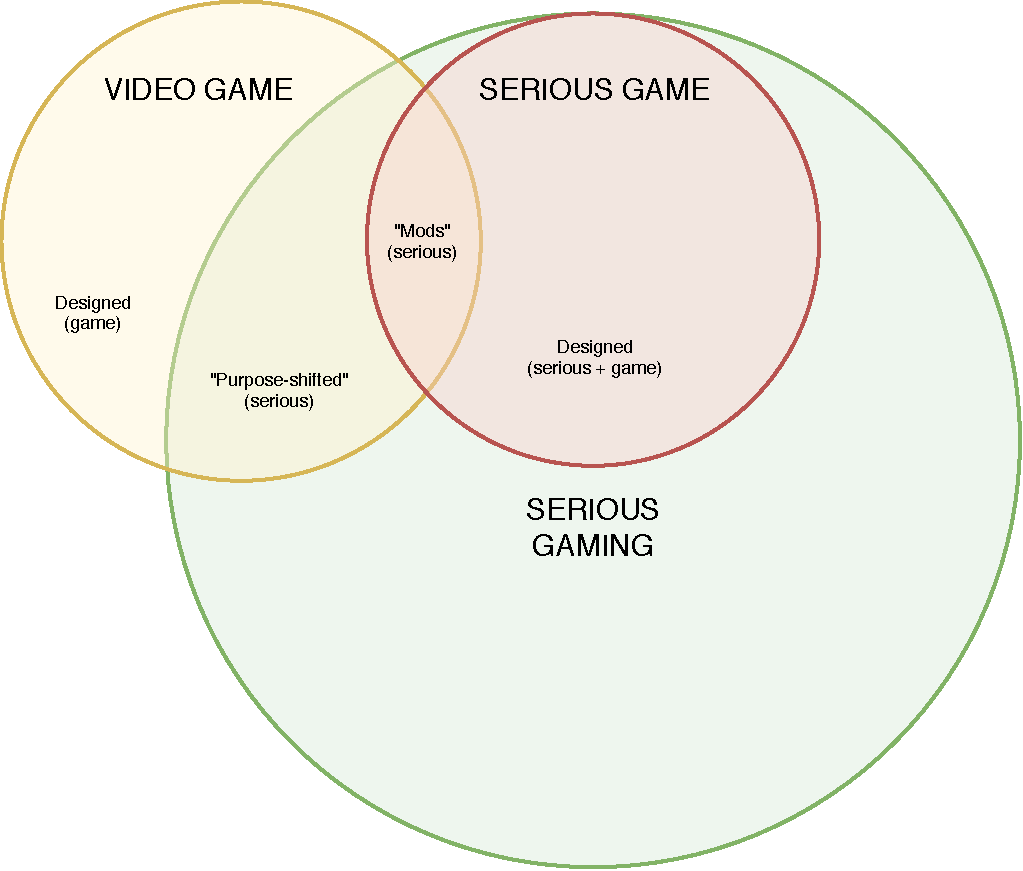
\includegraphics[scale=0.5]{Immagini/serious_gaming.pdf}}
\caption{Grafico che riassume la correlazione tra giochi, Serious Game e Serious Gaming} \label{fig:serious_gaming}

\end{figure}

\subsection{Classificazione}\label{sec:classification}

I Serious Games appaiono una categoria abbastanza ampia e ricca di elementi. Si � reso necessario, quindi, un sistema di classificazione, in modo da poter identificare al meglio i vari giochi appartenenti alla categoria. Fin dal 2002, sono stati fatti diversi tentativi per introdurre altrettanti sistemi di identificazione. Ognuno di essi � stato creato con il preciso scopo di migliorare i difetti del sistema precedente, ma purtroppo nonostante i vari tentativi nessuno di essi si � imposto in maniera generale sugli altri.

In ordine cronologico, le prime metodologie di classificazione sono basati su un singolo criterio di valutazione e possono essere suddivisi in due categorie: 

\begin{description}

\item[Market-based]
in cui il principio di distinzione � dato dal mercato (ossia le persone che ci giocheranno) che utilizza il gioco in questione;
\item[Purpose-based]
dove la classificazione avviene a seconda dell'intento e dello scopo per cui ogni gioco � disegnato e creato.

\end{description}

Le limitazioni di questi metodi sono numerose, in primis il fatto stessi che si basano solo su un solo criterio di distinzione. Inoltre per la classificazione ``Market-based'' il problema principale � che avviene solo tenendo conto dell'uso a cui � destinato il gioco e non del loro effettivo contenuto. Questo inconveniente � stato superato con il metodo ``Purpose-based'', afflitto per� da un altro tipo di difetto: vi sono categorie troppo eterogenee che ne limitano l'affidabilit�.

Questi metodi, per�, hanno avuto il merito di aver ispirato gli studiosi Sawyer e Smith, tanto da creare nel 2008 un loro sistema di classificazione, basato su criteri multipli: il ``Serious Game Taxonomy'' (\cite{Sawyer_2008}). Con questo sistema si categorizzano i giochi secondo due principi:

\begin{description}

\item[Mercato:]
Organizzazioni governative e non governative, Difesa, Salute, Marketing e Comunicazione, Educazione, Settore aziendale, Settore Industriale;
\item[Scopo:]
Giochi per la Salute, Giochi per la Pubblicit�, Giochi per l'Allenamento, Giochi per l'Educazione, Giochi per la Scienza e Ricerca, Produzione, Giochi come Lavoro.

\end{description}

Come si pu� notare, questo sistema � una fusione di quelli precedenti e fa uso di entrambi i criteri di classificazione. Inoltre nella categoria ``scopo'' avviene una sotto-classificazione aggiuntiva, andando ad aggiungere una maggior complessit�. Tutto ci�, comunque, permette una miglior comprensione dei Serious Games tramite una categorizzazione pi� precisa. Ciononostante, anche questo sistema ha dei punti deboli: il criterio ``scopo'' spesso risulta non sufficientemente accurato per alcune tipologie di gioco e sono presenti delle categorie di ``mercato'' e ``scopo'' che risultano coincidenti tra di loro. 

Nonostante i difetti del loro sistema, resta comunque il fatto che l'idea lanciata da Sawyer e Smith di utilizzare pi� elementi di classificazione risulti abbastanza convincente, a tal punto da essere ripresa nel 2011 da parte di Damien Djaouti, Julian Alvarez e Jean-Pierre Jessel in \cite{Felicia_2011} [cap. 6, pp. 118-136]. Questi 3 studiosi riprendono i 2 principi di classificazione di Sawyer e Smith, a cui per� ne aggiungono un terzo, il ``gameplay''. Questo � un aspetto che caratterizza essenzialmente qualsiasi gioco, ma di cui bisogna tener conto anche in questo ambito, dato che non si pu� scindere completamente un Serious Game dalla sua dimensione ludica. Con il modello da loro teorizzato, i 3 studiosi tentano, quindi, di superare i precedenti sistemi il cui limite principale consiste nel focalizzarsi solo sulla parte ``Serious'', tralasciando quella del ``Game''. 

In i tre aspetti distintivi del modello (fig.\ref{fig:gpsmodel}) sono:

\begin{description}

\item[Gameplay:]
che riguarda al tipo di gameplay utilizzato nel gioco. In particolare, le informazioni fornite da questo criterio riguardano la struttura del Serious Game (come � giocato);
\item[Scopo:]
che riguarda allo scopo per cui � stato designato il gioco. In particolare, gli eventuali scopi, oltre all'intrattenimento, a cui � destinato il Serious Game (perch� � giocato);
\item[Ambito:]
che riguarda alle applicazioni a cui � rivolto il gioco. In particolare,il tipo di mercato in cui � inserito e il pubblico che ne fa utilizzo (da chi � giocato).

\end{description}

\begin{figure}[tbh]

\centerline{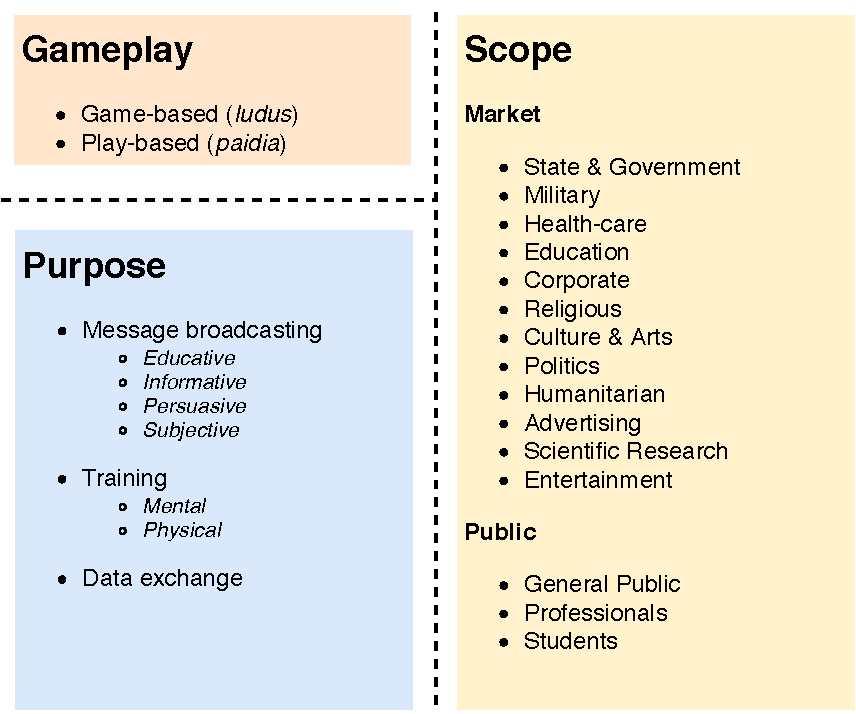
\includegraphics[scale=0.6]{Immagini/gpsmodel.pdf}}
\caption{Modello G/P/S per la classificazione dei Serious Games; sono riportate anche le sottocategorie per ogni carattere distintivo} \label{fig:gpsmodel}

\end{figure}

Per dimostrare l'efficacia del modello, il ``G/P/S Model'' � stato utilizzato per la creazione di un database di Serious Game \cite{Ludoscience_2011} in cui sono stati raccolti pi� di 550 Serious Games. Inoltre, essendo di natura collaborativa, se un prodotto risulta mancante all'interno della lista di giochi, � possibile aggiungerlo, classificandolo secondo lo stesso sistema.

Resta comunque anche esso un modello con dei limiti. Dato che � stato ideato per dare una visione generale dei Serious Games, non � possibile fornire informazione dettagliate su una specifica area d'interesse. Ad esempio, se si cerca un Serious Game associato al mercato dell'educazione, non possiamo differenziare tra quelli che trattano di matematica e quelli che trattano di storia. La differenziazione pu� avvenire solo secondo i criteri specificati dal modello. Ci� non toglie che pu� essere uno strumento utile per il Serious Gaming, dato che permette di identificare sia i vari Serious Games, che normali prodotti d'intrattenimento a cui � stato applicato un ``purpose-shifting''.  
 
\subsection{Vantaggi derivanti dal loro utilizzo\label{sec:benefits}}

In questa sezione si esporranno i possibili vantaggi derivanti dall'utilizzo dei Serious Games. Gli aspetti benefici sono stati studiati (e tutt'ora continuano ad esserlo) ormai da numerosi scienziati nel corso degli anni. � ormai confermato il fatto che utilizzare videogiochi possa aiutare ad aumentare le capacit� di problem-solving, affinare il pensiero strategico e migliorare l'attenzione, la vista e la coordinazione, a seconda dell'area di cervello attivata dal gioco in questione \cite{Subrahmanyam_1994}. 

Inoltre in campo medico si fa sempre pi� ricorso ai videogiochi sia per questioni legate alla riabilitazione fisica \cite{Lohse_2013, Bonato_2005} , cos� come per combattere problemi psicologici: fobie, paure, disturbo da stress post-traumatico (PTSD) \cite{Elliott_2015, Saraiva_2007} o disturbo da deficit di attenzione e iperattivit� (ADHD) \cite{Frye_2017, Kulman_2014}. Questo grazie anche al progresso tecnologico che ha permesso una sempre pi� elevata immersione del paziente nel mondo virtuale.

Ovviamente, cos� come sono stati condotti studi sugli aspetti positivi, ne sono stati fatti altrettanti per analizzare i possibili effetti negativi derivanti da un uso improprio dei videogiochi. � stato documentato infatti che un utilizzo prolungato in periodi brevi pu� portare il giocatore ad assumere comportamenti aggressivi \cite{Anderson_2010} o, addirittura, in alcuni casi, ad un distaccamento dalla realt�, causando l'insurrezione di patologie mentali (stress, ansia, depressione) e fisiche (obesit�). Questi sintomi, nel 2018, sono stati ufficialmente identificati all'interno dell'undicesima revisione della Classificazione Internazionale delle Malattie (ICD-11) dal World Health Organization (WHO) come ``gaming disorder'', malattia appartenente alla famiglia dei disturbi mentali e comportamentali \cite{ICD11_2018}. C'� da sottolineare, comunque, come quest'ultimo fatto sia stato ampiamente criticato e ritenuto prematuro, data anche la limitatezza di dati a supporto della teoria \cite{Aarseth_2017}.

Comunque sia questi ultimi aspetti negativi sono pi� legati all'utilizzo di videogiochi in generale che a quello dei Serious Games. Inoltre,ai vantaggi sopracitati, bisogna aggiungere anche i benefici derivanti dalla loro natura pedagogica. I principali vantaggi sono:

\begin{description}

\item [Coinvolgimento]
Come � stato pi� volte sottolineato, i Serious Game sono innanzitutto dei videogiochi ed � indubbio che molte persone si divertano nel giocarli, con la conseguenza di spendere molto tempo in questa attivit�. Ci� � dovuto principalmente al coinvolgimento, generato dal divertimento, che un videogioco ben strutturato riesce a creare nel giocatore. � possibile sfruttare questo aspetto per mantenere alto il livello di concentrazione di uno studente, evitando distrazioni dovute a poco interesse e noia.

Sebbene la sua importanza, il divertimento non � l'unico modo per coinvolgere il giocatore. Si possono sfruttare anche altri aspetti psicologici per aumentare il coinvolgimento. Ad esempio, la curiosit�, che pu� spingere un utente ad immergersi di pi� nel mondo virtuale solo per esplorarlo e scoprire tutti gli aspetti creati dagli sviluppatori.  
 
Ma il metodo pi� efficace per garantire un buon coinvolgimento da parte di chi gioca � quello di creare continue sfide. Proponendo degli ostacoli da superare, degli obiettivi da raggiungere, � possibile mantenere alto il livello di concentrazione dell'utente, che prover� un senso di soddisfazione ogniqualvolta riuscir� a completare una sfida, gettandosi nella risoluzione di quella successiva. Questo aspetto � stato soggetto di studio da parte di numerosi studiosi. Tra questi, Mihaly Cziksentmihalyi in \cite{Cziksentmihalyi_1988} e in \cite{Cziksentmihalyi_1991}, esplora ed espone i diversi stati mentali che una persona pu� attraversare nel momento in cui si trova coinvolto in un'attivit� che richieda delle abilit� e includa delle sfide. Una rappresentazione grafica � riportata in figura \ref{fig:flow_theory}. 

\begin{figure}[tbh]

\centerline{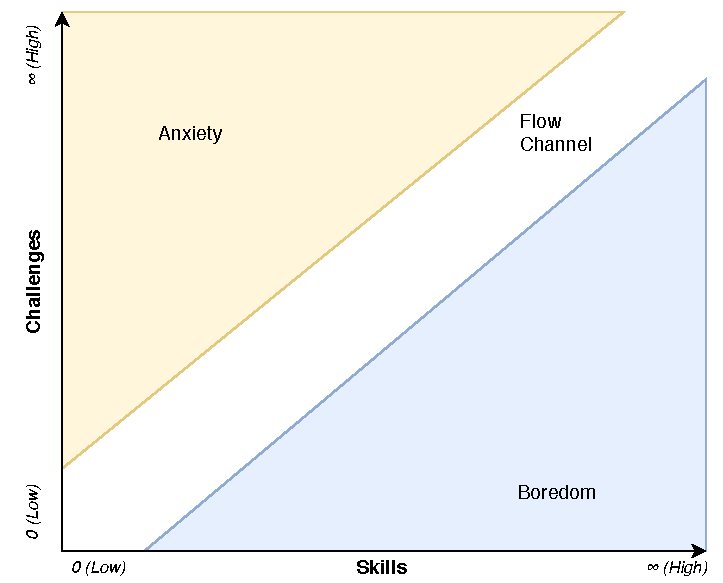
\includegraphics[scale=0.65]{Immagini/flow_theory.pdf}}
\caption{Grafico raffigurante la Teoria del Flusso di Cziksentmihalyi} \label{fig:flow_theory}

\end{figure}

Uno sviluppatore di un Serious Game deve essere capace di mantenere il giocatore all'interno del cosiddetto ``Canale di Flusso'', tenendo alta la motivazione. Questa infatti rappresenta l'elemento chiave per cui l'apprendimento possa avvenire. Per fare ci�, oltre a proporre delle sfide, il Game designer deve anche contemplare un sistema di feedback che renda l'utente consapevole dei propri progressi e del raggiungimento degli obiettivi, coinvolgendolo attivamente nel processo di apprendimento. Il gioco, inoltre, riduce l'ansia associata al compimento degli errori, visti non pi� come un fallimento che impedisce i progressi, ma come una fase necessariamente da attraversare per imparare. Naturalmente, al fine di ottenere i risultati migliori, il contesto del gioco in cui si cerca di raggiungere questo grado immersione e coinvolgimento deve essere il pi� vicino possibile ad un contesto del mondo reale.

\item[Apprendimento situato e contesto]
Nel 1991 Jean Lave e Etienne Wenger propongono in \cite{Lave_1991} una rivisitazione del concetto di apprendimento: i due studiosi affermano che questo non si sviluppa solo se indotto dall'insegnamento, ma anzi � un processo che si ottiene in determinati contesti, rapportandosi con altre persone (andando, quindi, a formare una comunit� di ``practioners'') e in relazione al coinvolgimento in attivit� specifiche. In questo senso, l'apprendimento � il risultato di ci� che viene definito dagli autori come ``legitimate peripheral partecipation'', ossia un processo attraverso il quale i neo-membri di una comunit� di ``practioners'', svolgendo inizialmente compiti semplici e poco rischiosi, acquisiscono gradualmente tutte le competenze necessarie per diventare esperti, finendo per essere coinvolti in ogni attivit� e pratica della comunit�.

Sulla base di questa teoria, negli anni a seguire, alcuni studiosi hanno cercato di trovare un'applicazione anche in campo informatico. In particolare, nel 2000, Jan Herrington in \cite{Herrington_2000} espone una lista di 9 features per identificare un modello di apprendimento situato, definendo poi un framework per il design degli ambienti d'insegnamento. Questi principi sono:

\begin{enumerate}

\item
Fornire contesti che rispecchino il modo in cui le conoscenze verranno usate nella realt�;
\item
Fornire attivit� realistiche;
\item
Permettere l'accesso alle performance di esperti;
\item
Fornire ruoli e prospettive multiple;
\item
Supportare la costruzione di conoscenza collaborativa;
\item
Promuovere la riflessione;
\item
Rendere esplicita la conoscenza tacita; 
\item
Fornire l'aiuto e il sostegno degli insegnanti nei momenti critici;
\item
Fornire giudizi durante le attivit� di insegnamento.

\end{enumerate}

Ancora, nel 2004, David Williamson Shaffer in \cite{Shaffer_2005} sottolinea la potenza che pu� generare il mondo virtuale dei videogiochi e come questo renda possibile lo sviluppo dell'apprendimento situato, permettendo allo studente il confronto con molteplici contesti in cui imparare concetti anche complessi, senza per� perdere di vista la loro relazione con i problemi del mondo reale. 

Il contesto di un Serious Game, inoltre, gioca un ulteriore ruolo di supporto nell'insegnamento dei concetti di teoria. In accordo con diverse teorie pedagogiche, insegnare non significa fornire solamente nuove informazioni. � necessario integrarle con il bagaglio conoscitivo dello studente, in modo che siano assimilate nella maniera pi� corretta. Inserendole nel giusto contesto, grazie anche all'immersione che si viene a generare, � possibile per il giocatore creare i legami con quanto gi� appreso, necessari per facilitare la memorizzazione dei nuovi concetti.

\item[Responsabilizzazione]
Molto spesso nei Serious Games, il giocatore viene catapultato in un contesto virtuale dove ricopre posizioni importanti dalle responsabilit� elevate. Questo comporta che dovr� prendere delle decisioni le cui conseguenze avranno un impatto nell'ambiente che lo circonda. Data la possibilit� di ricevere dei feedback visivi in tempi immediati, un giocatore pu� stabilire la corretta relazione causa-effetto delle sue decisioni, capire quali di esse fossero quelle corrette e rendere il processo di apprendimento pi� semplice e concreto.

\item[Necessit� di creare un modella della realt�]
Apprendere nozioni nel mondo reale pu� essere difficile anche a causa dei molteplici stimoli che una persona pu� ricevere, la maggior parte dei quali pu� anche risultare inutile. Nella creazione di un Serious Game (e pi� in generale di un qualsiasi videogioco), lo sviluppatore, per questioni legate al tempo e ai costi, deve adoperare delle operazioni di semplificazione della realt�, scegliendo cosa rappresentare fedelmente e cosa invece approssimare o ignorare. Questo comporta un vantaggio in termini di apprendimento, dato che il giocatore/studente si trover� ad interagire solo con gli elementi strettamente necessari per la sua formazione, evitando distrazioni causate dagli elementi superflui.

\end{description}

\section{Case study}{\label{sec:cases}

Come gi� affermato, nell'ultimo periodo, il boom dei Serious Games come strumento didattico si � diffuso anche in ambito informatico. A testimonianza � possibile confrontare la tabella 1 in \cite{Hendrix_2016} in cui � riportato una schematizzazione dei Serious Game per la cyber-sicurezza sviluppati negli ultimi anni. Nella stessa tabella, oltre a una breve tassonomia dei vari giochi, sono riportati anche i risultati ottenuti con il loro utilizzo. Come si pu� notare non tutti hanno registrato risultati, dovuto anche alla necessit� di avere ulteriori valutazioni, ma in generale � possibile affermare che il loro utilizzo abbia dato dei benefici. Tra quelli pi� positivi, ne sono stati scelti tre Serious Games da analizzare e di cui riportare le principali caratteristiche, anche in relazione con i concetti espressi fin ad ora.

\subsection{CyberCIEGE}

CyberCIEGE � un videogioco sviluppato nel 2006 da parte della Naval Postgraduate School per insegnare concetti di sicurezza delle reti. Il suo sviluppo � stato sovvenzionato dalla US Navy ed � attualmente utilizzato dagli stessi sviluppatori in corsi didattici, cos� come da numerose agenzie ed istituzioni scolastiche come strumento di addestramento. 

Il gioco � stato creato per permettere agli studenti di confrontarsi con delle decisioni a tema di sicurezza informatica, inserendoli in un ambiente sicuro e che incoraggia alla sperimentazione e alla riflessione. L'obiettivo � quello di mostrare i concetti astratti e le limitazioni dei vari meccanismi di difesa. Vi sono oltre 20 scenari che cercano di trattare il pi� possibile i vari concetti. Lo studente, nel gioco, ricopre il ruolo di amministratore di sistema di una qualche azienda e in ognuno degli scenari vi sono degli obiettivi da completare, il cui completamento potr� permettere l'avanzamento al livello successivo. Per far ci� dovr� prendere delle decisioni che possono potenzialmente intaccare la sicurezza dell'ambiente in cui lavora. Nei vari livelli, per completare i propri obiettivi, sar� necessario acquistare server aggiuntivi, creare permessi di rete specifici per permettere l'accesso alle risorse di sistema agli utenti indicati dal gioco, occuparsi della sicurezza fisica dei sistemi, educare le nuove risorse e cos� via. � presente, inoltre, un sistema di ricompense che premia il giocatore nel momento del raggiungimento degli obiettivi (altrimenti, in caso contrario, verr� punito tramite lo stesso). I principali elementi del gioco sono:

\begin{description}

\item[Asset]
L'insieme delle informazioni che il giocatore dovr� proteggere dagli attacchi. Possono essere sia fisiche che virtuali e ognuna di esse richiede un trattamento diverso, a seconda che se ne voglia mantenere la segretezza, l'integrit� o altre propriet�. Hanno un valore economico specificato che oltre a quantificare il danno che l'azienda subirebbe in caso di perdita della risorsa, caratterizza anche la frequenza degli attacchi subiti (pi� la risorsa sar� costosa, pi� frequentemente sar� attaccata).

Gli asset potrebbero dover essere condivisi all'interno dell'azienda, il che obbliga il giocatore a definire ed implementare una rete adatta affinch� ogni utente possa accedervi senza correre alcun rischio, tenendo anche conto della loro dislocazione sul territorio. Ci� comporta, se necessario, anche l'eventuale setup di una VPN o di altre misure di protezione nel caso in cui l'accesso all'asset avvenga tramite Internet.
\item[Utenti]
L'insieme degli impiegati virtuali presenti in ogni scenario. Come detto, al fine di completare gli scenari, � necessario che il giocatore fornisca loro le risorse di cui hanno bisogno, mettendoli nelle migliori condizioni di lavoro. A seconda del verificarsi o meno di queste condizioni, gli utenti possono assumere degli atteggiamenti diversi, a volte anche nocivi per la stessa azienda. Questo, unito anche al loro grado di abilit� nell'utilizzo delle le risorse, permette di distinguere quattro categorie di utenza diversa:

\begin{itemize}

\item
\textbf{Utenti normali} eseguono correttamente il loro lavoro utilizzando gli asset messi a loro disposizione. Possono apprendere nuove cose e migliorare la loro abilit�. Ci� non toglie che in caso di procedure particolari da eseguire, all'insorgere di un problema, tendono ad irritarsi, cercando degli escamotage potenzialmente pericolosi. Proprio per questo non � possibile garantire loro la gestione di dati particolarmente sensibili;
\item 
\textbf{Utenti affidabili} hanno un'abilit� pi� elevata rispetto agli utenti normali. Ci� comporta che possono trattare dati sensibili, ricoprendo ruoli di alta responsabilit�, e sono molto pi� tolleranti se messi di fronte a procedure complesse e restrittive da eseguire. Possono frequentare corsi speciali di aggiornamento;
\item 
\textbf{Utenti arrabbiati} sono utenti normali le cui richieste sono state ignorate (o non soddisfatte) dal giocatore. Cercheranno di recar danno all'azienda, cercando per� di non eseguire azioni troppo rischiose che comportino un loro licenziamento nel caso in cui vengano scoperti;
\item
\textbf{Utenti incompetenti} non hanno l'autorizzazione al trattamento di dati sensibili e generalmente non cercheranno di violare le politiche discrezionali dell'azienda. Tuttavia la loro incompetenza e l'ignorare i propri limiti li pu� portare a fraintendere la discrezionalit� di suddette politiche,causando danni ad informazioni a cui non dovrebbero nemmeno aver accesso.

\end{itemize}

In poche parole, quindi, il giocatore � tenuto a gestire si i rischi esterni che potenziali rischi interni alla stessa azienda, dovuti a comportamenti dannosi degli utenti arrabbiati e/o inesperti.
\item[Attaccanti]
Sono coloro che cercheranno di perpetrare gli attacchi, sia fisici che virtuali, ai danni dell'azienda. Sono suddivisi in due categorie principali:

\begin{itemize}

\item
\textbf{Vandali} elementi spinti principalmente dalla noia e/o dalla pura curiosit� tecnica. Non hanno motivazioni particolari che li invogli a spendere grosse risorse nell'attacco, ma hanno le competenze necessarie per danneggiare esplicitamente gli asset. Alcuni possono essere spinti in realt� solo da intenti sperimentali e non si rendono conto della pericolosit� delle loro azioni. Ci� non toglie che la loro presenza nei sistemi aziendali comporti l'intraprendere di azioni riparatorie da parte del giocatore;
\item
\textbf{Attaccanti professionisti} sono spinti da motivazioni prettamente economiche e, pertanto, hanno la propensione ad investire sia le risorse che il tempo nell'attacco. Cercano di effettuare attacchi clandestini la cui rintracciabilit� risulti difficile da parte del giocatore.Tenteranno, inoltre, di infiltrarsi sia all'interno dell'azienda (facendo assumere dei loro agenti o corrompendo gli utenti gi� presenti) che all'interno delle compagnie partner fornitrici di software, in modo da poter installare Trojan Horse o trap door nei sistemi aziendali, cos� da garantirsi l'accesso agli asset voluti. 

\end{itemize}

\item[Zone]
Ogni scenario � suddiviso in una o pi� zone, corrispondenti, ossia, alle suddivisioni fisiche dell'ambiente di lavoro. � possibile definire per ogni zona una politica di accesso, pi� o meno restrittiva, per ogni tipo di utente, definendo anche cosa si pu� portare al suo interno e cosa no. Per aiutare a rispettare queste regole, si possono utilizzare meccanismi di protezione aggiuntivi, quali porte magnetiche (il cui meccanismo di sblocco pu� essere basato su sistemi biometrici) o guardie di sicurezza.

Gli utenti si possono muovere tra le zone rispettando le regole definite. Tuttavia occorre considerare che la rete aziendale si si estende attraverso zone multiple. Ci� significa che, in caso di attacco andato a segno, � possibile per gli attaccanti ottenere l'accesso virtuale anche a zone proibite. Occorre quindi proteggersi ed evitare il verificarsi di questa situazione, utilizzando le risorse messe a disposizione dal gioco, come ad esempio dispositivi per la cifratura della rete o l'instaurazione di una VPN.
 
\end{description}

Il gioco inoltre mette a disposizione del giocatore 2 ulteriori strumenti, aumentando la profondit� del gameplay. Il primo � lo Scenario Development Tool (SDT). In poche parole � possibile produrre dei file di testo, scritti in Scenario Definition Language (SDL), per definire e descrivere degli scenari aggiuntivi, in modo da coprire quegli argomenti che non sono trattati in quelli predefiniti. Il linguaggio SDL descrive gli scenari in termini di utenti, asset, obiettivi degli utenti, attacchi e motivi per cui avvengono e impostazioni di sicurezza iniziale. Una volta definito ci�, il motore di gioco crea la topologia di rete, le impostazioni di sicurezza e, a partire dalla definizioni degli attacchi, stabilisce se essi andranno a buon fine o meno. gestir�, inoltre, in maniera automatica l'economia del gioco, lasciando quindi lo sviluppatore libero da questo compito. Ovviamente � necessario specificare un'ambientazione e gli obiettivi per completare lo scenario, in modo da permettere al giocatore di procedere attraverso una sequenza di sfide coerente e ben organizzata.

Il secondo strumento � una modalit� di gioco alternativa: mentre normalmente ci si ritrova nei panni di chi deve difendere e prevenire gli attacchi alla rete gestita, nella modalit� alternativa � possibile ricoprire il ruolo dell'attaccante, dando quindi la possibilit� di vedere la rete creata precedentemente da una nuova prospettiva. Il nuovo ruolo ricoperto permette di dimostrare l'effettiva protezione garantita dai metodi difensivi implementati ai vari tipi di attacco, cos� come l'efficacia di quest'ultimi. Anche in questo caso � richiesta al giocatore una buona capacit� decisionale per scegliere le tattiche di attacco pi� adatte, i cui esiti saranno subito mostrati, permettendo di valutare la tenuta difensiva della rete.

La valutazione del giocatore avviene su due livelli: il primo,pi� superficiale e immediato, � collegata all'andamento dell'economia del gioco. Prendere delle decisioni sbagliate, infatti, comincer� a far perdere fondi alla propria azienda, portandola ben presto sull'orlo della bancarotta (e di conseguenza alla fine del gioco). Al contrario, le decisioni corrette aiuteranno a generare introiti e permetteranno l'avanzamento ai livelli successivi. Oltre a questo, alla fine di ogni scenario viene mostrato al giocatore un log, riassumente tutte le decisioni prese durante il gioco, opportunamente analizzati dal sistema stesso, in modo da mettere in risalto le motivazioni dietro ad una determinata decisione. Questo pu� anche essere usato dagli insegnati, per registrare i progressi di uno studente e gli errori nei vari scenari. I log sono disponibili anche nel momento in cui si giochi uno scenario creato tramite lo SDT. Lo sviluppatore pu� configurare opportunamente dei trigger in modo da generare le parti di log nel momento in cui si verifichi una determinata situazione.

Nel corso degli anni, CyberCIEGE ha ottenuto ottimi risultati come strumento didattico, come dimostrano anche i risultati degli studi condotti sul suo utilizzo \cite{Jones_2010, Raman_2014, Krassmann_2015}. La sua efficacia � dovuta a vari fattori: innanzitutto il giocatore/studente ricopre, all'interno del gioco, un ruolo dall'elevata responsabilit�. Ci� spinge ad affinare la propria abilit� di individuare le giuste scelte da prendere nei vari contesti. Altri aspetti positivi sono sia l'immediatezza con cui sono presentati gli argomenti, mettendoli all'interno di un contesto ben delineato e soprattutto facilmente riconducibile alla realt�, sia la prontezza con cui vengono fornite le valutazioni. Inoltre la possibilit� di creare scenari personalizzati, cos� come quello di cambiare il ruolo, permettendo quindi di affrontare gli argomenti da una nuova prospettiva, danno una profondit� aggiuntiva al gameplay, offrendo ulteriori spunti di apprendimento. 

Ovviamente non � esente da difetti: il gioco richiede che il giocatore abbia una discreta conoscenza degli argomenti trattati, pena la difficolt� di giocare anche negli scenari pi� semplici. Inoltre dal punto di vista grafico si potrebbe aumentare la chiarezza di alcuni menu ed interfacce, rese alcune volte in maniera confusionaria, tramite l'utilizzo di informazioni aggiuntive e/o messaggi di suggerimenti. Ciononostante, la praticit� che lo caratterizza e l'immersione che si viene a generare dal suo utilizzo lo rendono uno strumento didattico molto valido e dall'alta efficacia.

\subsection{Anti Phishing Phil}

Anti Phishing Phil � un videogioco sviluppato nel 2007 da un team del CyLab Usable Privacy and Security Laboratory, facente parte della Carnegie Mellon University. Il gioco � stato supportato dalla US National Science Foundation per portare avanti l'iniziativa, da loro promossa, per aumentare la consapevolezza dei pericoli informatici \cite{CUPS_web}. Nel 2008 � stato acquistato dalla Wombat Security Technologies ed � tuttora da loro venduto, insieme ad altri prodotti, come strumento per il training. Nel 2009, il dipartimento di stato USA lo ha utilizzato per la formazione di oltre 55000 dipendenti \cite{Clarke_2009}. 

La teoria presente all'interno gioco verte su un solo argomento, di cui per� molto spesso si sottovaluta l'importanza: il phishing e le tecniche ad esso legate. Lo scopo � quello di educare la gente a riconoscere le trappole informatiche ed evitare di farsi ingannare, in modo da garantire la sicurezza dei dati sensibili, che siano quelli personali o aziendali. Il gioco ha un gameplay molto semplice ed intuitivo: al suo interno ci si ritrova a vestire i panni di un pesce chiamato Phil, imbattutosi in un gruppo di esche. A ogni esca � associato un URL, di cui occorre determinare la legittimit�. In caso di indirizzo associato ad un sito phishing, lo si deve scartare in modo da non venire pescati e perdere le proprie vite. In caso contrario � possibile mangiare l'esca, guadagnando punti. 

Il gioco � strutturato in quattro stage differenti, in ordine crescente per difficolt�, che vertono ognuno su diversi tipi di URL ingannevoli. Durante il gameplay, sono forniti al giocatore dei suggerimenti e delle indicazioni per mezzo di un altro personaggio (il padre di Phil). Per aumentare il grado di sfida, inoltre, sono inseriti all'interno di ogni scenario dei pesci nemici. Se Phil dovesse entrare in contatto con uno di loro, verrebbe mangiato e perderebbe una vita.

L'approccio allo sviluppo del videogioco si � diviso in 2 fasi, come riportato in \cite{Sheng_2007}: innanzitutto gli sviluppatori hanno individuato quali argomenti erano interessati a far assimilare al giocatore. In particolare, la scelta � ricaduta su tre aspetti:

\begin{enumerate}

\item
come identificare gli URL associati a siti di phishing;
\item
dove trovare degli indizi per poter identificare se un sito web � affidabile o meno;
\item
come utilizzare i motori di ricerca per individuare i siti web validi.

\end{enumerate}

Una volta definiti questi concetti, per far si che gli utenti riuscissero a recepirli in maniera corretta, gli sviluppatori hanno attinto dalle scienze pedagogiche, applicando i principi di:

\begin{itemize}

\item
\textbf{Riflessione:} ossia il processo tramite cui lo studente si focalizza mentalmente su ci� che sta apprendendo. Secondo degli studi, riportati in \cite{Sheng_2007}, l'apprendimento tramite Serious Games aumenta se, durante il gameplay, sono presenti dei momenti in cui i giocatori hanno la possibilit� di riflettere sulle nuove conoscenze apprese. Nel caso di Anti-Phishing Phil, il principio � applicato con la visualizzazione, alla fine di ogni livello, di un report con indicati i siti analizzati durante lo scenario, fornendo per ognuno di loro la corretta descrizione della loro natura;
\item
\textbf{Agenti story-based:} gli agenti sono elementi che aiutano e supportano lo studente durante il processo di apprendimento. Secondo questo principio, utilizzare degli agenti contestualizzati all'interno della storia del gioco migliora l'apprendimento. Le persone infatti tendono ad assimilare pi� informazioni se presentate in maniera organizzata e con dei rapporti causa-effetto, esattamente come accade quando si racconta una storia.In questo caso, Phil (il protagonista della storia e alter-ego del giocatore) rappresenta l'agente in questione;
\item
\textbf{Conoscenza concettuale-Conoscenza procedurale:} questi due tipi di conoscenze si influenzano a vicenda in maniera continua e danno vita ad un processo iterativo che dura per tutto il processo di apprendimento. All'interno del gioco questo viene reso tramite l'utilizzo di consigli procedurali specifici (es. ``URL con numeri all'inizio sono solitamente truffe''), affiancati da conoscenze concettuali (es. spiegazioni sulle parti che formano un URL e quali sono le pi� importanti).

\end{itemize}

L'apprendimento del giocatore, basato sui principi appena esposti, all'atto pratico si sviluppa grazie all'ausilio di messaggi di training. Questi sono stati inseriti in quattro fasi/posti diversi all'interno del gioco:

\begin{itemize}
\item
\textbf{Feedback durante il gameplay:} messaggi che vengono mostrati nel momento in cui si effettua una scelta (mangiare l'esca o meno) e che offrono un riscontro visivo immediato alla decisione presa;
\item
\textbf{Suggerimenti da parte del padre di Phil:} � possibile richiedere l'aiuto del padre di Phil durante il gameplay. Questi rispondere dando dei consigli su cosa osservare per effettuare la giusta scelta. Occasionalmente potr� mostrare i risultati di una ricerca sul web associata all'URL in questione. Con questi tipi di messaggi si forniscono le conoscenze concettuali relative all'utilizzo di un motore di ricerca e all'identificazione degli indirizzi affidabili;
\item
\textbf{Report di fine livello:} alla fine di ogni livello si mostra un sunto dei risultati conseguiti durante la partita. A fianco delle scelte errate sono riportate spiegazioni sul perch� siano sbagliate e consigli su come identificare gli URL correttamente;
\item
\textbf{Tutorial tra livelli:} tra un livello e l'altro sono stati inseriti mini-tutorial per spiegare le restanti nozioni non coperte all'interno dei messaggi precedenti, soprattutto riguardo l'utilizzo dei motori di ricerca per identificare un sito inaffidabile.

\end{itemize}

All'interno di \cite{Sheng_2007} � riportato anche una statistica per dimostrare l'efficacia del videogioco: sono stati condotti degli esperimenti su pi� di 1000 candidati in un arco temporale che va da settembre 2006 fino a febbraio 2007. I dati raccolti mostrano come l'utilizzo di Anti-Phishing Phil sia utile per migliorare l'abilit� di riconoscere un sito di phishing da uno reale, soprattutto se paragonato ad altri metodi. I motivi di questi risultati, secondo le parole degli sviluppatori, sono da ricercare sia nel contenuto dei messaggi di training sia nella modalit� in cui � presentato questo contenuto. � indubbio infatti che, nonostante non utilizzi un contesto realistico capace di generare un'elevata immersione nel giocatore, Anti-Phishing Phil ha il pregio di presentare gli argomenti in maniera semplice e diretta, guidando il giocatore nell'apprendimento e rendendo i concetti facilmente assimilabili da chiunque. 

\subsection{\doxed}

\doxed � un Serious Game che differisce in maniera radicale dagli altri due casi appena studiati: � infatti un gioco di carte, di cui solo ultimamente � stata creata una versione per PC, disponibile sulla piattaforma digitale di Steam \cite{Doxed_Steam}. Sviluppato a partire dal 2012 da quattro studenti, Zachary Peterson, Mark Gondree, Kate Lockwood e Joe Welch, � stato parzialmente supportato dal National Science Foundation, con l'assegnazione di due premi, e ha dato il via al progetto di ricerca TableTop Security, con l'obiettivo di investigare sull'utilizzo di giochi sia in classe che al di fuori per l'educazione alla sicurezza informatica \cite{Doxed_Site, TTS_Site}.

Come riportato in \cite{Gondree_2013}, l'obiettivo per cui � stato creato \doxed � quello di permettere una sempre pi� ampia diffusione delle discipline legate alla sicurezza informatica, cercando in particolar di modo di coinvolgere gli studenti pi� giovani, cos� da farli avvicinare fin da subito a questa disciplina, largamente ignorata nei piani di studio delle scuole primarie e secondarie. Inoltre, durante le fasi di design, al fine di aumentare le probabilit� di successo, hanno puntato a rendere il gioco facilmente accessibile e giocabile (non � richiesta, infatti, alcuna conoscenza della materia da parte dei giocatori) e soprattutto lo hanno rilasciato sotto una licenza open-source, rendendolo di fatto completamente modificabile da parte di chiunque, in modo da rendere l'esperienza di apprendimento ancora pi� personale e coinvolgente.

Le meccaniche del gioco si basano su quelle di ``Forbidden Islan'', gioco da tavolo creato da Matt Leacock. I giocatori impersonano le figure di alcuni hacker e si trovano all'interno di una rete informatica (formata dalle carte) in cui devono trovare e collezionare quattro diversi asset. All'inizio del proprio � possibile intraprendere alcune azioni: compromettere un nodo, spostarsi su un nodo precedentemente compromesso e scambiare le carte con gli altri giocatori. Dopo di ci� si riceveranno delle informazioni (sotto forma di ulteriori carte) riguardanti la rete in cui ci si trova e le sue vulnerabilit�. � possibile impadronirsi di un asset scartando quattro carte che lo raffigurano mentre si occupa il corrispondente punto di cattura. Alla fine del turno di tutti i giocatori, la rete si aggiusta, modificando la propria connotazione. Questo sta a simboleggiare l'intervento di un amministratore di sistema che cerca di impedire l'attacco alle proprie risorse.

Dovendo essere un gioco da utilizzare all'interno di classi di studenti, \doxed adotta un approccio di tipo collaborativo, piuttosto che competitivo: questo per aumentare la coesione tra gli studenti e rispecchiare la cooperazione necessaria per lo svolgimento di progetti e lavori di gruppo. La terminologia utilizzata al suo interno � molto semplice, ma comunque efficace. Questo per cercare di non spaventare gli studenti, creando in loro confusione ed inutili incomprensioni, e al contempo stimolare la loro curiosit�. 

La rete, come detto, � rappresentata tramite le carte, ognuna delle quali identifica un particolare nodo. Sebbene sia suggerita inizialmente una topologia a cui far riferimento, � possibile creare e esplorare le configurazioni pi� disparate. I nodi raffigurano le componenti pi� classiche che formano una rete aziendale, quali server DNS, serve mail, firewall, gateway di VPN. Quest'ultimi richiedono delle azioni aggiuntive da parte del giocatore, per essere violati, proprio come le loro controparti reali. Anche l'iconografia usata si muove in questa direzione, cercando di rappresentare in maniera semplice la vasta diversit� dei client presenti all'interno di una rete aziendale (PC desktop, laptop, smartphone, tablet, ...).

I giocatori, in \doxed, assumono possono assumere i ruoli di diversi tipi di hacker, ognuno specializzato in un tecnica di attacca: malware, social engineering, cryptoanalisi, botnet ed altri ancora. � possibile, durante il proprio turno, pescare una carta ``zero-day exploit'', con si pu� compromettere immediatamente ed occupare un nodo della rete: questa abilit�, per�, pu� essere utilizzata una sola volta durante il gioco. Sebbene possa sembrare irreale che un ``zero-day exploit'' permetta di attaccare qualsiasi tipo di obiettivo, senza alcuna distinzione, � stata fatta questa scelta di rappresentazione per rinforzare l'idea che e minacce sono ovunque e � possibile effettuare un attacco in maniera abbastanza semplice. Ovviamente l'utilizzo singolo permesso dal gioco richiede la pianificazione di una strategia ben congegnata, tipicamente associato agli ``zero-days exploit''.

La rappresentazione dei difensori, invece, � lasciata alla dinamica di adattamento della rete. Questo permette di illustrare le sfide relative ad un approccio alla sicurezza di tipo ``penetrate-and-patch''. Inoltre i giocatori possono meglio capire che questa tecnica non previene futuri attacchi, dato che dopo un cambiamento della rete � possibile comunque trovare nuove vulnerabilit� per effettuare un nuovo tentativo di manomissione. La frequenza con cui avvengono le modifiche alla rete sono scandite da un contatore, simboleggiante la quantit� di attenzioni che sta ricevendo l'infrastruttura dai suoi amministratori. Se questa diventa troppo alta, c'� la possibilit� che la rete venga dismessa, causando la sconfitta di tutti i giocatori.

Anche in questo caso, sono state trovate delle limitazioni al gioco: \doxed, in accordo con quanto affermato dagli stessi creatori, offre una rappresentazione della realt� a tratti troppo semplicistica. Le categorie degli asset rappresentati sono state scelte in maniera arbitraria, la rappresentazione fornita dei dati si focalizza solo su alcune propriet� di sicurezza (ignorando completamente altre), la rete � anch'essa rappresentata in maniera approssimata e viene fornita un solo approccio difensivo che � quello del ``penetrate-and-patch'', ignorando altre tecniche come i trusted system, meccanismi di difesa attivi o adattivi. Ciononostante, \doxed risulta un gioco molto adatto per approcciare l'argomento della sicurezza informatica, soprattutto per chi ha conoscenze limitate al riguardo. Sebbene la rappresentazione della realt� offerta � a tratti molto semplicistica, riesce a coinvolgere i giocatori, offrendo loro molti spunti di riflessione, offrendo la possibilit� di iniziare un dialogo tra ci� che � stato osservato nel gioco e gli attacchi che avvengo nel mondo reale.

\chapter{Sistemi SCADA}

Con questo capitolo si cercher� di fornire un'analisi generale sui sistemi SCADA. Innanzitutto, nella sezione \ref{sec:whatis} verr� data la definizione generale di cosa sia un sistema SCADA e per quali scopi � principalmente utilizzato. Nella sezione \ref{sec:architecture} verr� fornita una descrizione dell'architettura generica di un sistema di questo tipo, analizzando le componenti presenti in un sistema SCADA tipo e come si affronta la loro implementazione. Infine, nella sezione \ref{sec:scadaevolution}, si confronter� gli SCADA con una tipologia di sistemi di controllo simili, i DCS. Verr� fornita anche una panoramica sull'evoluzione tecnologica che ha inevitabilmente influenzato anche il campo dei sistemi di controllo e come questa abbia portato alla definizione del concetto di ``servizi SCADA''.

\section{Cosa � un sistema SCADA\label{sec:whatis}}

La definizione di sistema SCADA � contenuta all'interno dello stesso acronimo che viene utilizzato per identificare un tipo particolare di sistemi di controllo industriale, o ICS (Industrial Control System).  SCADA � l'abbreviazione di ``Supervisory Control and Data Acquisition'', ovverosia un sistema il cui scopo � di supervisione, controllo e acquisizione dei dati (funzionale ai fini dello svolgimento delle altre due operazioni). Gli scenari di utilizzo sono i pi� vari: dai classici sistemi di distribuzione e/o produzione energetica (impianti nucleari), ai sistemi di controllo fluidi (impianti di gestione della rete idrica/fognaria), ai sistemi di controllo del traffico, ferroviario e/o automobilistico, fino a sistemi geograficamente pi� contenuti, ma che necessitano comunque di controlli costanti (impianti di produzione industriale, stazioni di servizio, ecc.). 

Dalla definizione data, per�, non si riesce ad estrapolare cosa differenzi un sistema SCADA da un generico impianto di controllo distribuito (Distributed Control System, da qui in avanti DCS). Esistono infatti numero sistemi di controllo la cui classificazione � basata su diversi parametri, quali complessit� dei processi controllati, distribuzione geografica pi� o meno ampia, distribuzione dell'intelligenza di controllo, tempo di reazione disponibile al verificarsi di un evento prodotto dal sistema stesso, modalit� di interazione tra umani e macchinari e molti altri fattori ancora. Per capire veramente queste differenze occorre innanzitutto analizzare nel dettaglio come vengono svolti i tre compiti fondamentali (acquisizione dati, supervisione e controllo) e quali elementi, in generale, sono presenti nell'architettura di un sistema SCADA.

\subsection{Supervisione (Supervisory)}

La supervisione � la funzione principale a cui ogni sistema SCADA deve asserire (� possibile affermare che, senza supervisione, un impianto di controllo non pu� essere classificato come sistema SCADA). Tramite questa funzione � possibile monitorare lo stato in cui si trova il processo controllato e quale sar� la sua evoluzione. Per tale scopo, sono implementate tutte quelle funzionalit� che permettono di visualizzare le informazioni che descrivono lo stato attuale del processo, cos� come sono utilizzate delle strutture dati al cui interno sono raccolte le cosiddette informazioni storiche, che descrivono tutti i possibili stati assumibili dal processo durante la sua evoluzione. Tutto ci� � particolarmente utile nel momento in cui occorre identificare un eventuale stato anomalo del processo.

\subsection{Controllo (Control)}

Il controllo � la funzione che permette al sistema SCADA di prendere delle decisioni, in relazione allo stato attuale del processo controllato e alle sue future evoluzioni. Ovviamente questo compito pu� essere svolto in modalit� differenti, ma la cui definizione dipende principalmente dal tipo di processo controllato, a seconda del quale � necessario creare un'architettura sia hardware che software specifica per il compito. Una concetto molto importante � che in un sistema SCADA il controllo del processo � concentrato per la maggior parte all'interno dell'unit� di elaborazione (controllo centralizzato). In questo senso, l'elaboratore si serve del sistema di acquisizione dati per ottenere le informazioni ottenute dalla funzione di supervisione. Una volta elaborati queste dati grezzi (che non sono nient'altro che una rappresentazione dello stato del processo) se � necessario, cambia il valore dei parametri di stato che definiscono il processo di controllato, sfruttando sempre il sistema di acquisizione, ma nel senso opposto.

\subsection {Acquisizione Dati (Data Acquisition)}

L'acquisizione dei dati, sebbene sia di supporto alle precedenti funzioni, � quella che ricopre all'interno di un sistema SCADA una posizione fondamentale. � importante sottolineare che acquisizione dati, in questo contesto, sta ad identificare uno scambio bidirezionale tra l'unit� di controllo e quella di supervisione. Vi sono casi in cui l'acquisizione dati � il compito principale di un sistema SCADA, poich� il controllo e la supervisione possono essere realizzate in maniera pi� superficiale o anche a posteriori. Esempi di questi tipo sono forniti sono i sistemi di telerilevamento, in cui si raccolgono dati che verranno, eventualmente, con modalit� non sempre costanti.

In generale, per�, l'acquisizione ha un ruolo funzionale allo svolgimento degli altri due compiti di un sistema SCADA. Senza scambio dei dati, infatti, l'unit� di elaborazione non pu� avere le informazioni sullo stato attuale del processo, cos� come il sistema di supervisione non ricever� i valori dei parametri di controllo con cui gestire l'evoluzione dello stato del processo. 

Lo scambio deve avvenire nella modalit� pi� semplice possibile, senza alcuna manipolazione e/o elaborazione di sorta durante il percorso. Il processo di controllo avr� luogo all'interno del sistema di elaborazione. Ovviamente esistono situazioni in cui, le elevate dimensioni geografiche del processo controllato non permettono l'utilizzo di una sistema di controllo centralizzato, ma richiedono l'utilizzo di un sistema ad ``intelligenza distribuita''. In questo caso, per�, non siamo pi� di fronte ad un sistema SCADA.

\subsection{Analisi del processo da controllare}

L'architettura di un sistema SCADA generalmente � sempre la stessa ed � costituita da delle componenti che si possono definire ``standard''. Al momento della definizione delle caratteristiche funzionali di un sistema SCADA, per�, non si pu� ignorare il fattore rappresentato dal processo controllato. A seconda del tipo di analisi che si vuole condurre su di esso, infatti, si vanno a definire i vari parametri progettuali dell'impianto SCADA, sia quelli di tipo tecnologico che di tipo organizzativo. In questo senso, � utile classificare il processo da controllare in base a delle caratteristiche che aiuteranno poi a definire le funzioni fondamentali del sistema di controllo. \pagebreak

\begin{description}

\item [Tempo di reazione]
 Con questo parametro si stabilisce con quanto ritardo � in grado di reagire il sistema di controllo ai cambiamenti di stato del processo durante la sua evoluzione. Solitamente, nei sistemi SCADA, si parla di reazioni ``real-time'', ossia che abbiano un ritardo trascurabile, anche se pu� capitare che questa caratteristica vada in contrasto con altri aspetti legati al sistema di controllo. Il primo tra questi � il limite dovuto alla tecnologia con cui si realizza il sistema di acquisizione dati. Un esempio di quanto detto � dato dagli impianti di controllo con grandi dimensioni geografiche dove, a causa di ci�, il trasporto delle informazioni avr� un tempo che non sar� mai non trascurabile ed andr� ad introdurre un ritardo nelle reazioni dell'intero sistema SCADA. Un'altra criticit� pu� essere data dalla complessit� dell'unit� di elaborazione, spesso necessaria per soddisfare i vincoli di affidabilit� e disponibilit�, necessari per una corretta operativit� dell'intero sistema SCADA.
 Per cercare di conciliare tutti i vari requisiti sono adottate diverse soluzioni, a seconda del risultato pi� conveniente per il caso in cui operer� il sistema SCADA:
 
 \begin{itemize}
 
 \item ridurre i tempi di reazione solo per una certa parte degli eventi generati da un processo;
 
 \item ridurre la complessit� delle funzioni implementate nell'unit� di elaborazione, e pi� in generale la complessit� dell'intero sistema SCADA;
 
 \item utilizzare soluzioni tecnologiche ad hoc per il contesto in cui il sistema SCADA operer�.
 
 \end{itemize}
 
\item [Affidabilit�]
L'affidabilit� (intesa come ``reliability'') � un parametro altrettanto importante quando si parla di sistemi SCADA, di cui non si pu� fare a meno. Essendo utilizzati una grande quantit� di componenti, ognuno dei quali con il proprio grado di affidabilit�, al momento dell'implementazione del sistema occorre tenere conto di ognuno di questi valori. Ci� serve a stabilire le contromisure necessarie per evitare che, nel momento in cui si verifichi un malfunzionamento, questo influenzi l'intero impianto SCADA. Questo discorso vale sia per componenti di terze parti, di cui � sempre consigliabile verificare l'affidabilit� dichiarata dal produttore, sia per parti auto-prodotte, per la cui realizzazione ci si dovrebbe affidare a strumenti adeguati cercando di ottenere un grado di affidabilit� soddisfacente per l'utilizzo a cui � destinato.

Una considerazione da fare, quando si parla dell'affidabilit�, � che, in alcuni casi, cercare di ottenere un grado elevato di questa propriet� pu� risultare troppo oneroso e con risultati non sempre all'altezza della cifra investita. Un eventuale guasto, infatti, potrebbe anche non pregiudicare il corretto funzionamento di un sistema di controllo, se questo avviene entro particolari condizioni. Un esempio � dato dagli impianti di rilevamento ambientale, in cui in caso di perdita di dati, si pu� parlare di evento trascurabile, se l'intervallo di tempo interessato dal disservizio � breve rispetto al tempo totale in cui il sistema ha lavorato.
 
\item [Disponibilit�]
Con questo parametro si indica il tempo totale in cui il sistema di controllo ha garantito il corretto funzionamento del processo controllato. Ovviamente, come nel caso dell'affidabilit�, anche la disponibilit� si pu� riferire all'intero sistema come alle singoli parti che lo compongono. In generale il soddisfacimento dei vincoli imposti dipende dal tipo di processo controllato: si possono avere situazioni con vincolo molto stringenti, cos� come processi per cui la disponibilit� � una caratteristica che passa in secondo piano (ma comunque si avranno sempre dei vincoli da rispettare al momento dell'implementazione del sistema SCADA) 

\item [Interazione uomo-macchina]
Data la presenza di sistemi di controllo e supervisione, � necessario implementare anche un sistema con cui si fornisce ad un operatore la possibilit� di interfacciarsi con l'impianto SCADA. Questi sono spesso indicate con la sigla HMI (Human Machine Interface), la cui complessit� dipende, come per tutti gli altri parametri, dal processo controllato dal sistema SCADA. Per impianti in cui sono utilizzate procedure completamente automatizzate, baster� un'interfaccia che sia semplicemente in grado di permettere l'osservazione dei vari stati evolutivi del processo. D'altra parte, nei casi in cui, oltre all'osservazione, � richiesto all'operatore di effettuare anche operazioni di controllo, � necessario un'interfaccia che implementi tutte le funzionalit� richieste per svolgere il compito assegnato, senza per� andare ad inficiare sulla facilit� di utilizzo, che deve rimanere in ogni caso adeguatamente alta.

In passato, vi erano casi particolari in cui era impossibile realizzare un qualsiasi tipo di interfaccia, per via delle numerose informazioni da riportare a schermo. Oggi, grazie all'utilizzo di monitor dalle grandi dimensioni o, se necessario, di ``video wall',' questi casi sono sempre meno frequenti.

\item [Dimensione geografica]
Anche in questo caso, la dimensione del sistema � strettamente vincolata dalla dimensione geografica in cui ha luogo lo svolgimento processo. Se, ad esempio, parliamo di un processo con un'area geografica limitata, come pu� essere una linea di produzione industriale o un sistema di depurazione, il sistema SCADA pu� essere collocato interamente in un unico edifico, solitamente lo stesso che ospita il processo da controllare. Se invece prendiamo in considerazione il controllo di un sistema di trasporto energetico, la cui dimensione � chiaramente vasta, � necessario che il sistema SCADA rispecchi la distribuzione geografica del processo stesso, in modo da rendere lo svolgimento del lavoro pi� semplice. Ovviamente, in questo caso, aumenta la complessit� architetturale dell'impianto di controllo, in quanto si rende necessario affrontare le varie criticit� che sono introdotte dalla presenza delle notevoli dimensioni in cui tutta l'operazione si svolge. Una su tutti � l'affidabilit� dei sistemi di comunicazione, che deve risultare sempre molto alta, poich� un'eventuale corruzione delle informazioni trasportate potrebbe pregiudicare completamente le operazioni di controllo. Altra criticit� pu� essere rappresentata dalla presenza di pi� postazioni di controllo, soluzione utilizzata in particolari casi di processi dalle elevate dimensioni geografiche. In questo caso occorre realizzare un adeguato sistema di interfacce uomo-macchina che permette l'accesso contemporaneo ai dati, senza incorrere in errori dovuti all'inconsistenza delle informazioni salvate nei database. 

\end{description}

\section{Architettura di un sistema SCADA\label{sec:architecture}}

In generale, l'architettura di un sistema SCADA � composta da tre sottosistemi adibiti allo svolgimento dei rispettivi compiti di controllo, supervisione e acquisizione dati. Questi sono denominati come:

\begin{itemize}

\item sistema di elaborazione dati, adibito al controllo del processo;
\item sistema di trasmissione dati, destinato allo svolgimento delle funzionalit� di acquisizione dati;
\item sistema di acquisizione, a cui � assegnato il compito di supervisione.

\end{itemize}

Come � possibile notare in figura \ref{fig:scadaarchitecture}, nella zona pi� periferica � presente il sistema di acquisizione, mentre quella centrale � destinata al sistema di elaborazione. La comunicazione tra questi due sottosistemi � garantita grazie al sistema di trasmissione dati.

\begin{figure}[tbh]

\centerline{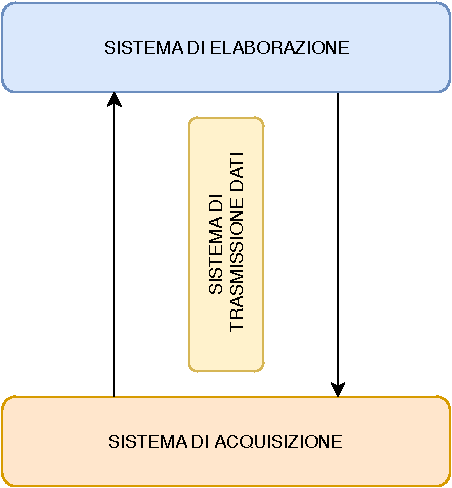
\includegraphics[scale=0.8]{Immagini/scada_architecture.pdf}}
\caption{Rappresentazione grafica dell'architettura di un generico sistema SCADA}\label{fig:scadaarchitecture}

\end{figure}

Come per il caso del sistema SCADA in generale, l'implementazione di questi tre sottosistemi � specifica per il tipo di processo a cui sono destinati ( e pu� risultare a volte molto complessa), ma se ne pu� dare comunque una definizione generica, individuando gli elementi che caratterizzano ognuno di essi.

\subsection{Sistema di elaborazione}

\begin{figure}[tbh]

\centerline{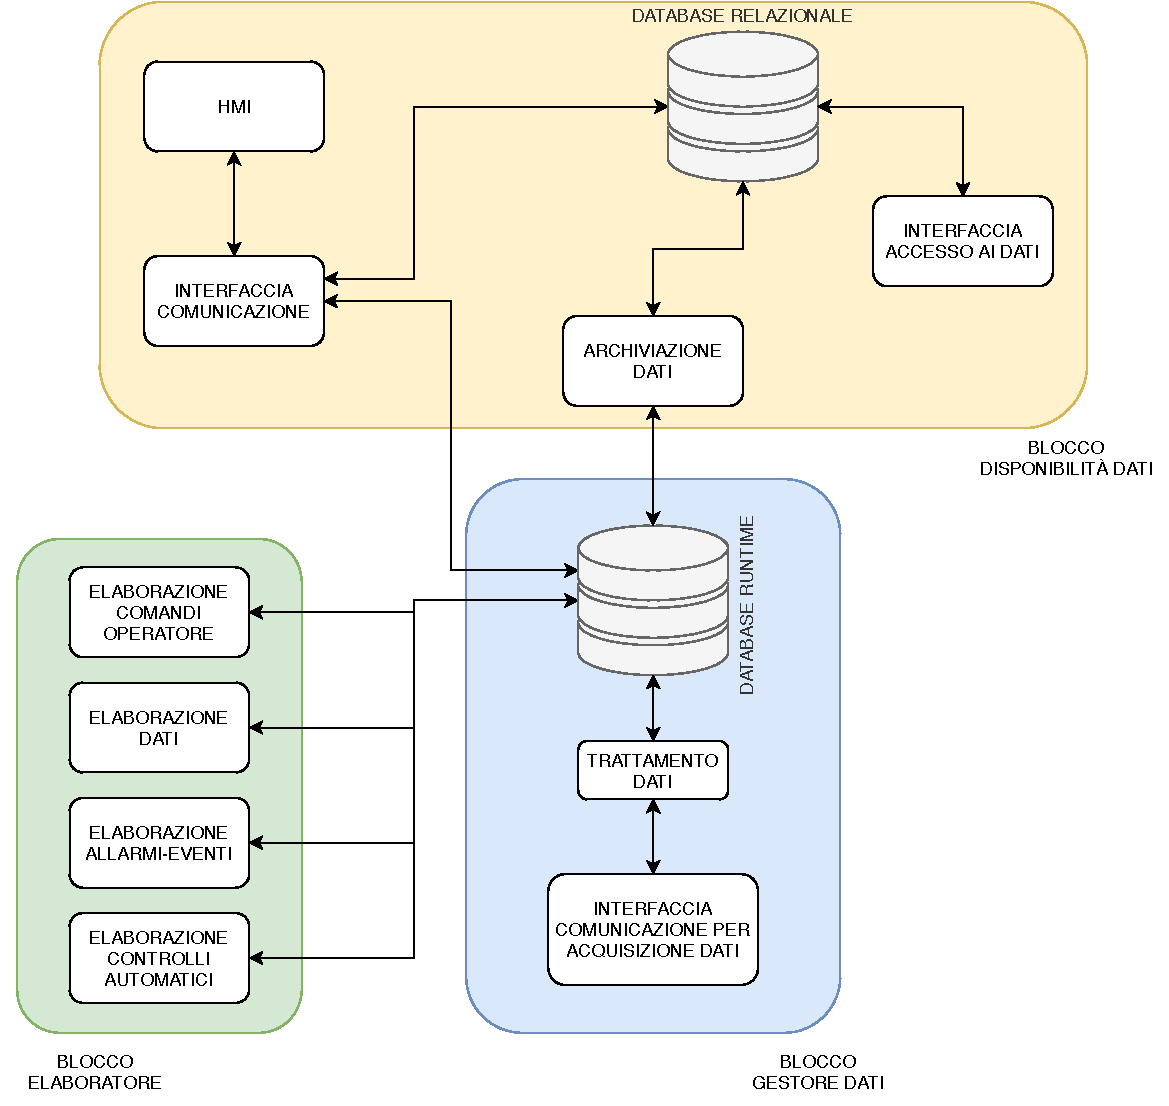
\includegraphics[scale=0.75]{Immagini/elaborator_architecture.pdf}}
\caption{Rappresentazione grafica dell'elaboratore di un sistema SCADA}\label{fig:elaboratorarchitecture}

\end{figure}

In \ref{fig:elaboratorarchitecture} � riportato uno schema a blocchi dei componenti presenti in un elaboratore. Come � possibile vedere, in generale i vari componenti di un elaboratore possono essere raggruppati in tre macro-blocchi: quello preposto alla gestione dei dati, quello il cui compito � di garantire la disponibilit� delle informazione e il blocco elaborativo vero e proprio. Di seguito verranno analizzati in maniera pi� dettagliata le funzionalit� che caratterizzano ognuno dei blocchi. \pagebreak

\begin{description}

\item [Gestore dati]
Il compito delle componenti per la gestione dei dati � quello di comunicare con le apparecchiature periferiche (sia per raccogliere i dati necessari all'elaborazione che per inviare i dati elaborati necessari per le azioni di controllo), trattare i dati per renderli interpretabili dal sistema e archiviare le informazioni, sia grezze che gi� elaborate. Tutte queste operazioni costituiscono il cuore di tutte le alte funzionalit� del sistema SCADA.

I dati riguardanti lo stati del processo da controllare sono ricevuti dalle apparecchiature di controllo e sono subito tradotti nel formato di riferimento del sistema interno (ovviamente, nel momento in cui occorre comunicare con l'esterno avviene il procedimento inverso, in cui le informazioni sono tradotte nel formato adeguato affinch� siano utilizzabili per effettuare le varie azioni di controllo). Il flusso di queste informazioni, sia in entrata che in uscita, ha come punto di raccolta il ``database runtime'', che viene chiamato in questo modo proprio per il fatto che opera in tempo reale con la dinamica evolutiva del processo controllato. � implementabile in vari modi (ad esempio, pu� essere costituito da aree di memoria condivisa tra i vari processi di controllo), ma l'importante � che soddisfi tutte le richieste ricevute da parte del sistema di elaborazione in tempi ridotti. Tramite ci� vengono, quindi, garantite le funzionalit� di controllo e supervisione del sistema SCADA. Ovviamente, per motivi di sicurezza e per permettere lo svolgimento di azioni di supporto al controllo del processo, � consigliabile mantenere questi dati e salvarli per un eventuale utilizzo successivo. A tale scopo viene utilizzato, parallelamente al ``database runtime'', un ``database relazionale'', che rappresenta il componente principale del blocco adibito a garantire la disponibilit� dei dati.

\item[Disponibilit� dati]
Come detto in precedenza, al fine di permettere lo svolgimento di azioni di supporto a quelle di controllo, spesso si rivela utile utilizzare un ``database relazionale'' in cui salvare tutti i dati, si quelli ricevuti dall'esterno che quelli elaborati dal sistema stesso. Le azioni di supporto possono essere le pi� svariate, dalle analisi legate ai dati descrittivi degli stati del processo, in modo da poter svolgere funzioni di correzione preventiva, alle gestione e consultazione di dati dal carattere economico. Ovviamente, in questo caso non � richiesto che il database lavori in tempo reale. Ha molta pi� importanza che le informazioni abbiano un'elevata intelligibilit�, vi siano gli strumenti di accesso necessari per garantire la disponibilit� dei dati e infine che il database riesca a gestire facilmente le grandi quantit� di informazioni salvate al suo interno. Tutto ci� permette agli operatori ed ai sistemi esterni di fare accesso ai dati senza coinvolgere direttamente il sistema di controllo e supervisione.

\item [Elaboratore]
Il blocco dell'elaboratore � quello preposto alla manipolazione ed interpretazione dei dati descrittori dello stato evolutivo del processo. Questo blocco, una volta ricevute le informazioni dall'esterno (fornite dal ``database runtime''), effettua un'analisi su di essi ed invia come risposta una serie di comandi per il controllo del processo. Ovviamente questa analisi pu� essere fatta dagli operatori umani, ma spesso la grande quantit� di dati da analizzare, corrispondente di solito a processi da controllare dall'elevata complessit�, rendono necessario l'utilizzo di procedure di supporto. Queste producono, sostanzialmente, una serie di informazioni aggregate insieme ad una sintesi dei vari comandi da poter inviare al processo controllato. Ovviamente vi sono anche altre esigenze che questi processi elaborativi di supporto devono poter soddisfare, tra queste le pi� importanti sono:

\begin{itemize}

\item generare segnalazioni di eventuali anomale presenti nell'evoluzione del sistema;
\item generare rappresentazioni sintetiche dello stato attuale e dell'evoluzione del processo;
\item interpretare i comandi forniti dall'operatore;
\item realizzare procedure di controllo automatiche.

\end{itemize}

Quest'ultimo punto si rende necessario nei sistemi SCADA adibiti al controllo di processi che non sono direttamente controllabili dagli operatori umani. In questo caso, il sistema compie delle azioni predefinite di controllo automatico con una cadenza periodica.

\end{description}

\subsection{Sistema di acquisizione}

Il sistema di acquisizione dati in un impianto SCADA rappresenta lo strumento tramite cui dialogare con l'esterno. Il suo compito principale � fare da traduttore tra il sistema centrale (l'elaboratore) e quello periferico, convertendo le informazioni analogiche, quali temperatura, pressione e tutte le altre grandezze che descrivono lo stato del processo, in informazioni binarie. Al fine di permettere una comunicazione corretta, � necessario, oltre a stabilire un linguaggio di comunicazione unico per tutto il sistema SCADA, anche definire le modalit� di comunicazione e la codifica da applicare alle informazioni scambiate. Ovviamente, le tipologie di sistemi di acquisizione possono essere delle pi� disparate, a seconda delle caratteristiche considerate per definire l'architettura del sistema SCADA. 

Al fine di individuare l'apparato di acquisizione dati pi� indicato per le proprie esigenze, � utile capire ed individuare la tipologia di informazioni che l'impianto dovr� gestire. Questa analisi pu� essere svolta in base ai seguenti criteri:

\begin{description}

\item [Direzione delle informazioni]
Sulla base di questo criterio � possibile effettuare una duplice distinzione. Abbiamo infatti le ``informazioni in ingresso'', ossia i dati che riceve, sia dal sistema centrale che da quello periferico, che le ``informazioni in uscita'', di nuovo, informazioni che possono essere dirette o al sistema centrale o agli apparati esterni. Ovviamente, � chiaro che vi � una relazione di equivalenza tra i vari dati gestiti. Le informazioni in ingresso dal sistema centrale, infatti, sono le stesse che, opportunamente tradotte, sono dirette in uscita verso l'impianto periferico (vale, chiaramente, anche l'equivalenza opposta, ossia informazioni in ingresso dal sistema periferico diventano quelle in uscita verso l'elaboratore centrale);

\item [Caratteristiche elettriche delle informazioni]
Questo criterio viene applicato quando sono prese in analisi le informazioni relative agli apparati periferici, che siano in entrata o in uscita. Affinch� il sistema riesca ad interpretare le informazioni, � necessario tradurre le grandezze fisiche in un segnale elettrico adeguato. Ci� � reso possibile grazie al lavoro svolto dai trasduttori, mentre per l'operazione inversa � richiesto l'utilizzo degli attuatori. Ovviamente � necessario che tutti gli apparati di acquisizione utilizzino lo stesso tipo di rappresentazione elettrica dei dati.

Vi sono molteplici standard industriali per ognuno dei segnali considerati, che siano digitali, analogici, in ingresso o in uscita. In generale, per i dati digitali, sono utilizzati dei segnali elettrici dal voltaggio variabile (il range va dai \SI{24}{\volt} ai \SI{220}{\volt}) a corrente sia continua che alternata, a seconda di ci� che � pi� adatto allo scenario in analisi. Per le informazioni analogiche, invece, i segnali utilizzati sono differenziati sulla base delle grandezze elettriche. Abbiamo infatti:

\begin{itemize}

\item misure in tensione;
\item misure in corrente;
\item misure in resistenza;
\item misure in termo resistenza;
\item misure in termo coppia.

\end{itemize}

Tutte queste informazioni sono rilevanti quando si va ad eseguire l'analisi per il corretto dimensionamento del circuito elettrico, in quanto descrivono le caratteristiche elettriche, come ad esempio l'assorbimento, dei vari trasduttori e/o attuatori.

\item [Qualit� delle informazioni]
In questo caso, il termine ``qualit�'' sta ad indicare quale � la tipologia dell'informazione gestita ed � necessario definirla al fine di garantire il loro corretto trattamento. � possibile eseguire questa distinzione in base a quattro macro-aree:

\begin{itemize}

\item \textbf{informazioni digitali:}
queste informazioni sono rappresentate come un insieme di dati binari. Sono associate alle grandezze fisiche che descrivono lo stato di un processo;
\item \textbf{informazioni analogiche:}
questa tipologia di dati � utilizzata per rappresentare le grandezze fisiche tramite una serie di valori oscillanti all'interno di un certo range. Sono richieste delle opportune conversioni analogico/digitale affinch� siano utilizzabili dall'elaboratore per svolgere le funzioni di supervisione e controllo;
\item \textbf{informazioni impulsive:}
questo tipo di informazione non � interpretabile in tempo reale. Piuttosto se ne richiede la conoscenza in un determinato arco temporale, in modo da ottenere una corretta rappresentazione della grandezza a cui sono associate;
\item \textbf{informazioni complesse:}
questo tipo di informazione � prodotto, usualmente, da dispositivi complessi con cui il sistema SCADA si interfaccia. Un esempio � fornito dai contatori elettrici di ultima generazione, che producono un'insieme di informazione relativamente a tensione, corrente, potenze, dati economici ed altro ancora, il tutto in relazione a diversi periodi temporali, pi� o meno lunghi. In questo caso, piuttosto che analizzare ed acquisire ognuno di quei dati in maniera indipendente come delle informazioni analogiche, � preferibile utilizzare interfacce apposite, in grado di stabilire la comunicazione con il dispositivo tramite protocolli di comunicazione ad hoc. Questo permette al sistema di acquisizione di comunicare con tutti i dispositivi esterni che utilizzano quel particolare protocollo, aumentando di fatto la compatibilit� del sistema stesso. Una volta stabilita la comunicazione, questa avviene in maniera autonoma, permettendo l'acquisizione delle informazioni. Tra i vari protocolli utilizzati, si segnalano il ``ModBus'', il ``ProfiBus'', il ``CanBus'' ed il ``LonWorks'', che risultano essere quelli pi� diffusi.

\end{itemize}

\end{description}

A livello pratico, questa analisi si traduce nei parametri di programmazioni da applicare ai PLC, ``Programmable Logic Controller''. Questi sono dei veri e propri computer componibili, la cui struttura hardware � adattata al processo da controllare. Il loro compito � gestire i segnali digitali ed analogici che transitano nella rete costituita dai sensori, gli attuatori e il sistema di elaborazione centrale. Negli ultimi anni, grazie anche alle progressive migliorie tecnologiche che ne hanno permesso una riduzione delle componenti fisiche e, conseguentemente, dei costi, si � cominciato ad utilizzare i PLC anche in ambiti domestici. Un esempio � la loro applicazione nei quadri elettrici delle abitazioni per gestire automaticamente i vari impianti presenti nelle case: riscaldamento, irrigazione, rete internet, ecc.

\subsection{Sistema di trasmissione dati}

I componenti sopra elencati necessitano di interfacce adeguatamente implementate per comunicare correttamente tra di loro. In un sistema SCADA occorre garantire la comunicazione tra:

\begin{itemize}

\item sistema di elaborazione e sistema di acquisizione dati;
\item sistema di elaborazione e sistema di gestione dati;
\item processo controllato e dispositivi di interazione (attuatori);
\item dispositivi di interazione e sistema di acquisizione dati.

\end{itemize}

Pu�, inoltre, rivelarsi utile implementare delle interfacce per comunicare con altri elementi esterni, quali sistemi gestionali dell'azienda o sistemi informativi in generale. Ognuna di queste interfacce dovr� essere implementata secondo le caratteristiche pi� adeguate per lo scopo a cui � destinata. Il rischio � quello di compromettere le normali funzionalit� del sistema SCADA o, addirittura, la sua realizzabilit�. Inoltre, in fase di progettazione, � consigliabile tenere conto anche dei possibili sviluppi futuri a cui potrebbe essere soggetto il sistema SCADA. Di seguito sono riportate le caratteristiche su cui basare l'analisi dei protocolli da applicare alle interfacce comunicative che si vogliono implementare.

\begin{description}

\item [Velocit�]
Uno degli aspetti pi� cruciali dei canali di comunicazione � quello di garantire una velocit� sufficientemente elevata, tale da rendere possibile che l'azione di controllo del processo avvenga in tempi ridotti ed adeguati. I vincoli imposti, in questo senso, sono spesso molto restringenti e ci� pu� costringere all'impiego di sistemi periferici ad intelligenza distribuita per compiere le azioni di controllo. Alcuni dei casi in cui questi problemi si verificano con costanza sono i sistemi SCADA con notevoli dimensioni geografiche. In questo caso occorre utilizzare le infrastrutture di comunicazione dei gestori telefonici, che normalmente sono destinate ad un impiego ``general purpose''. Ci� pu� rendere il servizio non sufficientemente adeguato per lo scopo finale e occorre, quindi, ricorrere a sistemi periferici con intelligenza di controllo distribuita, in modo da svolgere le azioni nei tempi richiesti.

Nel caso della comunicazione tra il sistema e le HMI, invece, la comunicazione deve avvenire sempre in ``real-time'', in modo da rendere pi� efficace il lavoro degli operatorio. Questo deve avvenire sia per la visualizzazione dei parametri descrittivi dello stato del processo, che per la risposta alle azioni di controllo attuate dagli operatori.

Infine, la comunicazione con i sistemi esterni � vincolata dal tipo di sistema con cui occorre interfacciarsi. Se � anch'esso un sistema di controllo, allora i vincoli sono gli stessi visti nel caso di comunicazione con il processo, con annesse limitazioni. Se, d'altra parte, si vuole comunicare con un sistema non di controllo, l'interfaccia da implementare non presenta delle particolari restrizioni da rispettare, anzi possono essere considerate come trascurabili.
� importante sottolineare come, di solito, non sia possibile soddisfare tutti i requisiti imposti dal tipo di comunicazione che si vuole implementare, scendendo di fatto ad un compromesso tra protocolli implementati e tecnologia utilizzata.

\item [Sicurezza]
La sicurezza � un aspetto altrettanto importante da considerare al pari della velocit�, soprattutto nel caso in cui le probabilit� di intrusione da parte di soggetti indesiderati siano abbastanza alte. Chiaramente, nel caso di un sistema chiuso, i tentativi di intrusione a cui si � soggetti diventano esigui, ma non bisogna scordare che � sempre presente la possibilit� di un errore umano da parte degli operatori. Si rende necessario, quindi, ricorrere ai ripari preventivamente, cercando di evitare il presentarsi di queste spiacevoli situazioni, che siano causati da attacchi intenzionali o errori in buona fede. 

La gestione della sicurezza deve riguardare sia le comunicazione tra elaboratore e sistema periferico di acquisizione dati, sia tra un sistema SCADA ed un altro, in quanto i entrambi i casi l'alterazione delle informazioni trasportate pu� provocare un comportamento anomalo da parte dell'impianto di controllo.

Tra le soluzioni adottabili, la pi� gettonata � la separazione delle diverse aree di lavoro accessibili al sistema ed agli operatori. Questa separazione pu� avvenire sia fisicamente, cos� come dal punto di vista dell'implementazione logica, ed in generale � dipendete dal tipo di tecnologia implementata per l'interfaccia di comunicazione. 

In ogni caso, il passo pi� importante da compiere � quello di definire un'adeguata politica di sicurezza fin dalle fasi progettuali, cosa che negli ultimi anni � diventata imprescindibile, ma che nel passato era trattato con molta superficialit�. Questo perch� mentre prima i sistemi SCADA erano isolati completamente dal mondo esterno, oggi fanno largo impiego di tecnologie comunicative pubbliche, dal basso costo, ma dalla sicurezza pi� debole. Si � reso necessario, quindi, un cambio di approccio al tema della sicurezza.

\item [Intelligibilit�]
L'intelligibilit� � un parametro importante nel momento in cui si vuole realizzare un sistema che interagisca costantemente con apparecchiature esterne per la supervisione ed il controllo. In questo caso � possibile applicare diverse soluzioni, ma le pi� adatte sono quelle che fanno riferimento a degli standard comunicativi predefiniti. Ci� � facilmente comprensibile sia dal punto di vista tecnologico, funzionale ed economico. 

Tecnologico e funzionale perch� un protocollo proprietario (ossia non standard) non � detto che sia utilizzato dai dispositivi con cui si vuole comunicare, restringendo quindi la gamma di apparecchi utilizzabili. Inoltre, non � detto che tra quelli effettivamente utilizzabili vi sia il dispositivo adatto a soddisfare tutte le esigenze di comunicazione richieste. Infine, economicamente parlando, un protocollo standardizzato ha dietro di s� il supporto di un'intera comunit� scientifica, mentre nel caso di uno proprietario si � costretti a sottostare alle esigenze di mercato dell'azienda padrona del protocollo.

\item [Affidabilit�]
In generale � richiesto che i dati trasmessi all'elaboratore del sistema SCADA mantengano un alto gradi di integrit�. Ci� per rendere possibile una corretta valutazione dello stato evolutivo del processo. Una soluzione potrebbe essere quella di applicare meccanismi di validazione dati nei dispositivi periferici, ma ci� rallenterebbe la risposta generale del sistema all'evoluzione del processo. L'unica opzione rimanente � integrare questi meccanismi nel canale di comunicazione, in modo da riuscire a garantire l'integrit� delle informazioni trasportate.

La soluzione ideale per rispondere a questo problema prevede l'implementazione di tre diverse funzionalit�:

\begin{itemize}

\item rilevazione degli errori;
\item richiesta di ritrasmissione in caso di errori rilevati;
\item ordinamento delle informazione all'interno del flusso dati.

\end{itemize}

Questi meccanismi sono implementabili nelle maniere pi� differenti, facendo ricorso agli algoritmi che pi� si ritengono adatti. Purtroppo, per�, l'introduzione di queste funzioni va ad intaccare la velocit� di comunicazione, richiedendo, quindi, il raggiungimento di un compromesso in grado di garantire un adeguato rapporto tra la rapidit� di scambio delle informazioni e il mantenimento della loro integrit�. Inoltre, per ottimizzare l'efficacia della soluzione adottata, � consigliabile lo svolgimento di un'attenta analisi del sistema di comunicazione in questione. � ovvio infatti che nel caso in cui la comunicazione avvenga su di un mezzo di per s� gi� affidabile, come la fibra ottica, si preferisce evitare l'implementazione di tecnologie per gestire gli errori di trasmissione, in quanto sarebbe praticamente inutilizzato. Se, invece, la comunicazione avviene su di un mezzo meno affidabile, come dei trasmettitori wireless, � fortemente consigliato l'impiego di funzionalit� di rilevamento e correzione degli errori.

Infine, nel caso in cui la comunicazione da stabilire sia tra pi� sistemi SCADA, l'aspetto che si prende pi� in considerazione � l'ottimizzazione dei costi di trasmissione, in quanto, come detto, sono presenti molti meno vincoli sulla velocit� e sull'affidabilit� dei dati scambiati.

\item [Disponibilit�]
In stretta correlazione con l'aspetto dell'affidabilit� vi � quello della disponibilit� dei dati trasmessi. In casi di disservizio del sistema di comunicazione, infatti, anche le operazioni di controllo, direttamente collegate alle comunicazioni, rischiano di subire dei malfunzionamenti. Occorre, quindi, garantire la continuit� della disponibilit� delle informazioni in quanti necessaria per svolgere correttamente le attivit� di controllo (per le quali � fondamentale conoscere in tempo reale lo stato del processo da controllare o, nel caso di attuazione di una politica di controllo, occorre prontamente informare l'attuatore dell'azione che dovr� intraprendere).

Le soluzioni pi� adatte partono tutte dall'assunzione di un principio molto importante: anche un sistema ad alta disponibilit� pu� interrompere il suo normale servizio per un guasto. In questi casi, per prevenire e combattere il verificarsi di una situazione del genere, si richiede l'utilizzo di protocolli comunicativi opportunamente scelti e la realizzazione di sistemi ridonanti, in cui i dispositivi restano a riposo fino al verificarsi di un guasto. In quel momento saranno prontamente messi in azione per sostituire le componenti ordinarie fuori servizio. Questa soluzione � adottata per tutti i dispositivi presenti nel canale di comunicazione.

\item [Supporto dei servizi]
Un'ulteriore aspetto da considerare nell'analisi del sistema di comunicazione � la tipologia delle informazione scambiate. � stato dimostrato, infatti, che a parit� di tipo di dati trasmesso, diverse tecnologie e protocolli offrono prestazioni diverse da loro. Occorre, quindi, analizzare se l'interfaccia scelta � adeguata a garantire una qualit� di comunicazione sufficientemente elevata per il tipo di dato che si vuole trasmettere.

\end{description}

\section{Differenze tra sistemi DCS e sistemi SCADA\label{sec:scadaevolution}}

Le componenti appena analizzate non sono una prerogativa dei soli sistemi SCADA, ma sono utilizzati nei vari sistemi di controllo, tra cui i DCS. Ci� che li differenzia, quindi, non � quali strumenti sono utilizzati, ma piuttosto come vengono implementati. In particolar modo ka disinzione � sul grado di distribuzione dell'intelligenza di controllo. I DCS, acronimo che sta ad indicare i ``Ditributed Control System'', come suggerisce gi� il nome stesso, sono basati sull'impiego di strutture di acquisizione dati, ma con anche un'elevata capacit� elaborative, creando di fatto un paradigma tecnologico contiguo delle funzioni di controllo e acquisizione, Negli SCADA, invece, come abbiamo visto, le due funzioni sono ben distinte ed affidate ad impianti separati, fisicamente e tecnologicamente.

Nel caso DCS, quindi, non si parla di apparecchiature di acquisizione, ma di unit� di elaborazione periferiche, in grado non solo di ricevere dati, ma anche di interpretarli, analizzarli per individuare lo stato attuale in cui il processo si trova e, se necessario, eseguire delle azioni di controllo sul processo. LA complessit� architetturale di queste unit� periferiche, cos� come le funzioni che sono in grado di svolgere, � basata sul tipo di processo che si deve controllare. L'unit� centrale di elaborazione, nel contesto di un sistema DCS, ha quindi il compito di acquisire sia informazioni grezze che informazioni gi� elaborate che danno indicazioni sullo stato delle strutture di controllo.

Osservando, per�, l'evoluzione tecnologica avvenuta negli ultimi anni che ha interessato anche l'ambiente dei sistemi di controllo, � possibile fare un riflessione sulla necessit� di mantenere o meno questa distinzione tra sistemi DCS e SCADA. Inizialmente, la distinzione era dettata dalle differenti caratteristiche tecnologiche che venivano implementate, spesso frutto di scelte obbligatorie per risolvere un particolare problema di controllo. Con lo sviluppo delle infrastrutture di comunicazione e delle tecnologie computazionali la scelta tra un sistema di elaborazione centralizzato con periferiche di acquisizione pure e un sistema con controllo ed elaborazione distribuito anche nelle apparecchiature di acquisizione � diventata sempre pi� una questione legata a fattori quali scalabilit� dell'impianto, grado di manutenzione da garantire e altre caratteristiche non inerenti alla effettiva realizzabilit� del sistema. A tal proposito, si prevede che a causa del continuo progresso tecnologico, la distinzione tra sistemi DCS e SCADA si far� sempre pi� assottigliata fino a sfociare nella creazione di un'unica categoria di classificazione, di cui entrambi faranno parte.

\subsection{Evoluzione tecnologica dei sistemi SCADA: integrazione con sistemi informativi aziendali}
L'evoluzione tecnologica che ha colpito e continua ad interessare i sistemi SCADA ha portato a due principali conseguenze:la prima � stata, come detto, la diminuzione del divario tra la categoria SCADA e quella dei DCS, creando dei sistemi ibridi in cui sono integrate funzionalit� di entrambe le parti. La seconda, altrettanto importante, � stata la definizione di nuove architetture con lo scopo di creare non pi� una paradigma che descriva un sistema fisico, ma piuttosto una funzionalit�. In tal senso, � utile vedere le diverse linee evolutive che sono state applicate per realizzare questa idea.

La prima � stata quella che permettesse l'integrazione tra un sistema SCADA con uno gestionale concorrente. In questo modo � possibile interagire direttamente con un sistema informatico aziendale, con il fine di fornire supporto automatizzando la gestione interna, sia organizzativa che contabile. In figura \ref{fig:integratedsystem} � possibile vedere un esempio di questo caso. Come � possibile osservare,le varie modalit� di comunicazione del sistema SCADA convergono tutte nel sistema informatico aziendale.

\begin{figure}[tbh]

\centerline{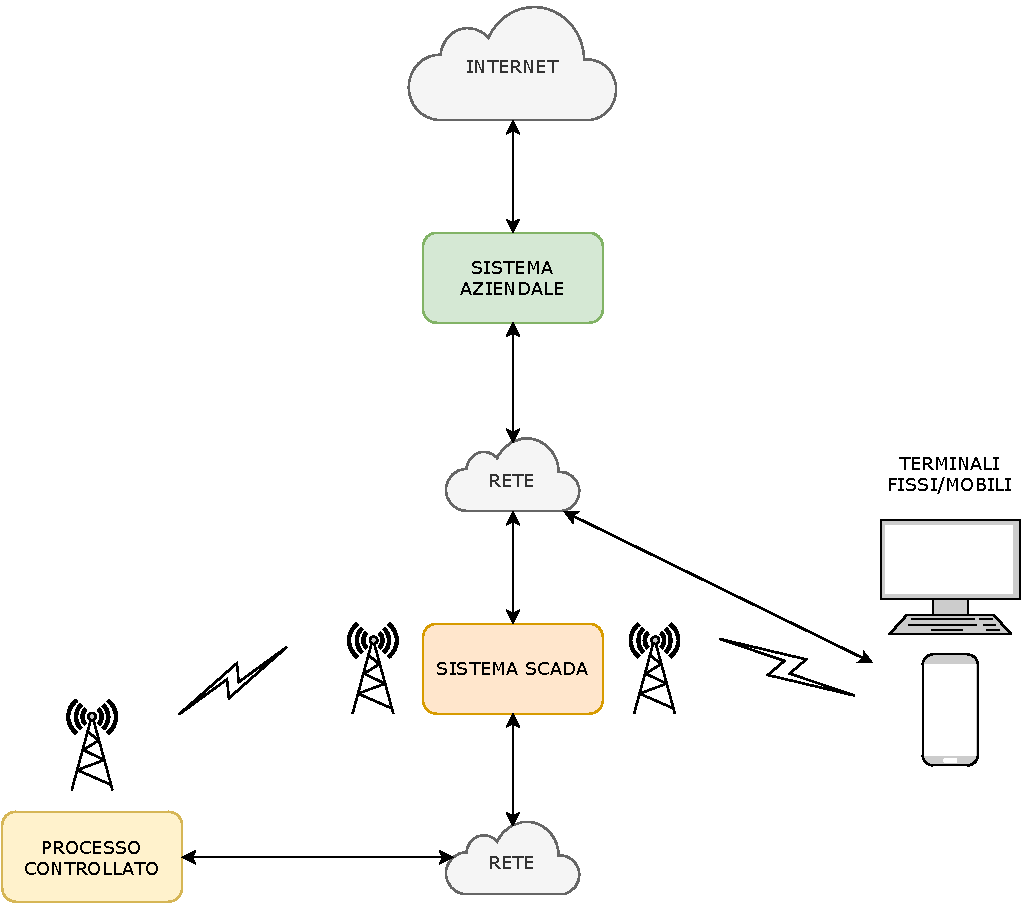
\includegraphics[scale=0.75]{Immagini/architettura_sistema_integrato.pdf}}
\caption{Architettura di un sistema SCADA integrato con un sistema aziendale}\label{fig:integratedsystem}

\end{figure}

Una volta progettata l'architettura, con le entit� che ne faranno parte, e le comunicazioni tra di esse, occorre analizzare di quali informazione il sistema aziendale ha bisogno per svolgere correttamente le sue funzioni. Il supporto che deve fornire, infatti, � ottimale solo se il sistema SCADA � in grado di fornire le informazioni corrette sullo stato del processo controllato. Un esempio pratico di quanto descritto pu� essere dato da un sistema SCADA integrato con il sistema gestionale di un magazzino. In questa situazione ipotetica, le decisioni su cosa ordinare e quanto sono prese basandosi sulle informazioni che sono fornite dal sistema SCADA riguardo lo stato del processo controllato. Se queste non fossero corrette, vi sarebbero delle decisioni prese in maniera errata che alla lunga porterebbero ad un danneggiamento economico alla stessa azienda. Questo elencato � solo uno dei molteplici casi in cui � possibile effettuare l'integrazione tra sistema aziendale e quello SCADA, automatizzando la gestione interna. Si possono fare considerazioni simili anche nel caso in cui ci si trova a fornire dei servizi tecnologici tramite web.

Un'altra linea evolutiva scaturita dal processo tecnologico riguarda lo sviluppo di sistema SCADA con larga estensione geografica. In questo caso, un grosso aiuto � stato dato dallo sviluppo delle comunicazioni e le tecnologie legate ad esse. Grazie alle reti ethernet e la tecnologia TCP/IP � stato possibile creare delle infrastrutture di comunicazione sempre pi� affidabili e soprattutto facilmente modificabili secondo le proprie esigenze. Queste, come detto, sono largamente utilizzate nelle strutture di comunicazione di un sistema SCADA. Inoltre si stanno integrando anche funzionalit� legate alla comunicazione radio: sempre pi� spesso si utilizzano comunicazione wireless per le trasmissioni locali, cos� come molti sistemi di controllo utilizzano la rete cellulare sia per comunicare con strutture difficilmente raggiungibili da una rete cablata che per avvisare gli stessi operatori nel caso in cui ci sia bisogno di un intervento urgente.

\subsection{Un nuovo paradigma: la creazione di servizi SCADA}

Una delle ultime evoluzioni scaturite dal miglioramento tecnologico � stato un cambio di approccio alla soluzione del problema della supervisione. Tradizionalmente, come visto, sono realizzati dei sistemi di controllo ad hoc la cui gestione � a carico degli operatori responsabili del processo controllato. Questa soluzione prevede prima una fase di analisi per individuare le esigenze di controllo, definire successivamente i requisiti del sistema e la sua architettura per poi, alla fine, passare alla fase di installazione hardware ed implementazione software. Il tutto chiaramente comporta un lavoro molto lungo e oneroso. 

Negli ultimi tempi, invece, si � applicata un diverso approccio per la ricerca della soluzione al problema sopra citato: il focus � stato spostato sulla realizzazione di servizi SCADA che rispondano a esigenze di tipo funzionale. In questo modo il servizio coinvolge due tipologie di operatori, in maniera diversa. Chi crea il servizio, ossia il fornitore, gestisce e controlla direttamente il sistema SCADA e dovr� occuparsi dei problemi architetturali e progettuali. Il committente, ovverosia il fruitore del servizio, non sar� coinvolto nella realizzazione dell'impianto, ma avr� il compito di gestire i problemi organizzativi nati dall'introduzione del sistema di controllo nella rete aziendale. Una configurazione tipica di un servizio SCADA � mostrata nella figura \ref{fig:scadaservices}, dove � possibile notare la separazione tra il fornitore ed il fruitore del servizio stesso.

\begin{figure}[tbh]

\centerline{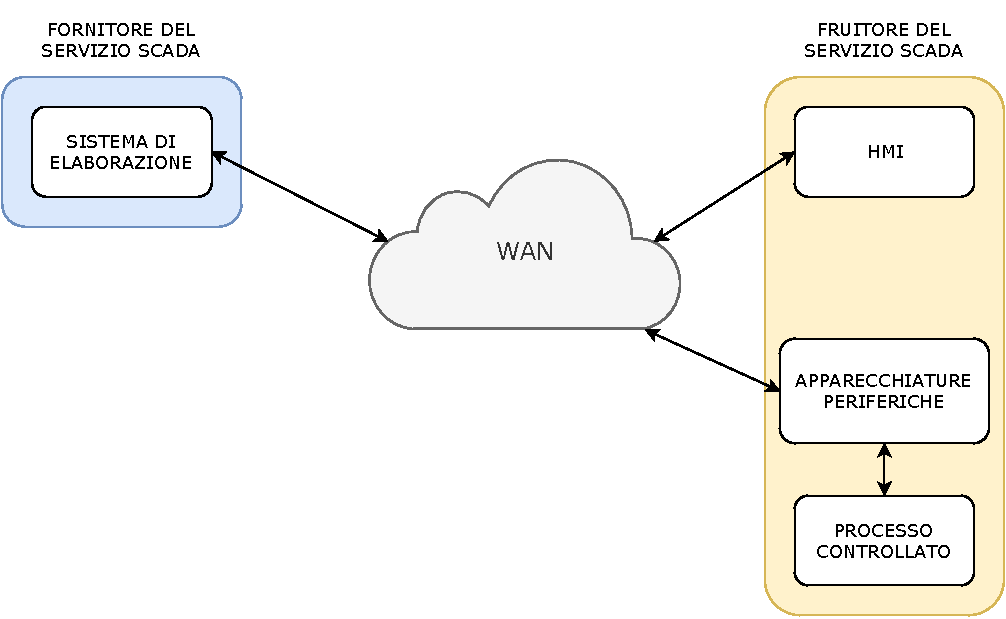
\includegraphics[scale=0.75]{Immagini/architettura_servizi_scada.pdf}}
\caption{Architettura di un servizio SCADA}\label{fig:scadaservices}

\end{figure}

Come si pu� notare dallo schema riportato, il sistema di elaborazione viene gestito dal fornitore. Questo sar� messo in comunicazione con le restanti componenti tramite una rete realizzata nelle vicinanze del processo ed accessibile tramite dei canali di comunicazioni simili a quelli utilizzati nei sistemi distribuiti. Il fruitore potr� accedere alle funzionalit� di supervisione e controllo del sistema SCADA tramite le interfacce HMI messe a disposizione dal fornitore.

Ovviamente, occorre tenere anche in considerazione gli aspetti legati all'affidabilit� del servizio, alle prestazione e, soprattutto, alla sicurezza. Se prima ci trovavamo spesso al cospetto di un sistema chiuso, creato ad hoc per rispettare le proprie esigenze, ora l'adozione di un servizio SCADA comporta il condividere molti dati con una terza parte esterna, rappresentata in questo caso dal fornitore. Questi dati, molto spesso, sono cruciali poich� permettono la realizzazione del sistema di controllo. Una loro eventuale perdita o manomissione comporterebbe dei danni sia economici che operativi molto elevati.

\chapter{Analisi dei rischi in un sistema SCADA}

In questo capitolo verr� analizzata la sicurezza di un sistema di controllo SCADA e di come i paradigmi di difesa siano cambiati con il progredire delle tecnologie utilizzate. Nella sezione \ref{sec:itsecurity} si provveder� a dare una panoramica sui concetti di sicurezza informatica che hanno particolare rilievo nei sistemi industriali e quali siano le differenze con la sicurezza IT domestica. Nella sezione \ref{sec:mobilesecurity}, invece, verr� trattato l'argomento dei dispositivi mobile utilizzati in ambiente SCADA e di come occorre preoccuparsi anche della sicurezza di questi dispositivi, molto spesso sottovalutata.

Successivamente, nella seconda parte del capitolo sar� affrontato l'argomento degli scenari di attacco che possono presentarsi: nella sezione \ref{sec:typicalattacks} verranno mostrate una serie di minacce, analizzando le loro modalit� di impiego e quali difese � possibile adottare contro di esse. Infine, nella sezione \ref{sec:stuxnet}, verr� effettuato il case study di una delle minacce pi� pericolose nell'ambiente SCADA: il worm Stuxnet con cui, nel 2010, � stato effettuato uno dei pi� grandi attacchi ai danni dei sistemi di controllo delle centrali nucleari iraniane da parte del governo USA \cite{Zetter_2015}.

\section{Sicurezza informatica in ambito industriale \label{sec:itsecurity}}

Come visto nel capitolo precedente, l'evoluzione tecnologica che ha investito i sistemi di controllo industriali ha portato all'utilizzo di numerose tecnologie IT, sia per questioni di efficienza funzionale che economica. Questa scelta ha comportato non solo la presenza di aspetti positivi, ma anche l'introduzione di tutte le criticit� tipiche del mondo IT. Di conseguenza, � aumentata l'apprensione per i temi di sicurezza, quali accessi non autorizzati, dati manomessi/perduti e attacchi alla rete o al sistema con conseguente malfunzionamento degli stessi; in altre parole tutte le criticit� che precedentemente avevano poca importanza poich� ci si trovava molto spesso in un sistema chiuso non accessibile dall'esterno, ora assumono una rilevanza molto alta.

Tradizionalmente, per l'ambiente domestico, esistono molte soluzioni ai suddetti problemi IT, tutte costantemente testate e modificate per migliorare la loro efficienza. Purtroppo, per�, queste soluzioni non possono essere applicate nello stesso modo agli ambienti industriali, in quanto di origine tecnologica diversa e soprattutto le criticit� da considerare sono diverse. Per questo motivo, nel 2002, fu istituito il comitato dell'``International Society for Automation'' (ISA) formato da esperti di sicurezza informatica industriale, con l'intento di stabilire delle linee guida per indicare quali metodi di difesa e ``best practices'' sono da adottare per mantenere la sicurezza dei sistemi di controllo industriale.

Il comitato stil�, come prima cosa, una lista al cui interno sono state raccolte le principali preoccupazioni che possono scaturire da un attacco informatico ad un sistema di controllo:

\begin{itemize}

\item danneggiamento della sicurezza pubblica e/o personale;
\item perdita di fiducia da parte del pubblico;
\item violazione di requisiti normativi;
\item perdita di informazione proprietarie e/o confidenziali;
\item perdita economica;
item impatti sulla sicurezza nazionale.

\end{itemize}

Finalmente, nel 2007, il comitato rilasci� la prima serie di schemi di certificazioni che furono pubblicati dall'``American National Standards Institute'' (ANSI) con il nome di protocollo ANSI/ISA99. Questo � stato ampliato e aggiornato nel coso degli anni fino al 2010, anno in cui il nome fu cambiato in ISA/IEC-62443. Il cambio fu effettuato per mantenere coerenza nella numerazione dei protocolli rilasciato dall'ANSI e il corrispettivo standard dell'``International Electrotechnical Commission''. Come � possibile notare dalla figura \ref{fig:isa99}, i report tecnici che compongono lo standard ISA/IEC-62443 sono suddivise in quattro macro categorie:

\begin{enumerate}

\item la prima (partendo dall'alto) � la categoria che include le informazioni di base, quali terminologie, modelli e concetti fondamentali;
\item la seconda � rivolta ai proprietari degli asset. Sono affrontati vari aspetti legati alla creazione e mantenimento di programmi per la sicurezza;
\item il terzo gruppo include una serie di documenti che tracciano delle linee guida per la progettazione dei sistemi di difesa. Sono inclusi anche dei modelli di riferimento per il design del sistema;
\item l'ultima categoria descrive lo sviluppo ed i requisiti tecnici da rispettare per i sistemi di sicurezza degli impianti di controllo.

\end{enumerate}

\begin{figure}[tbh]

\centerline{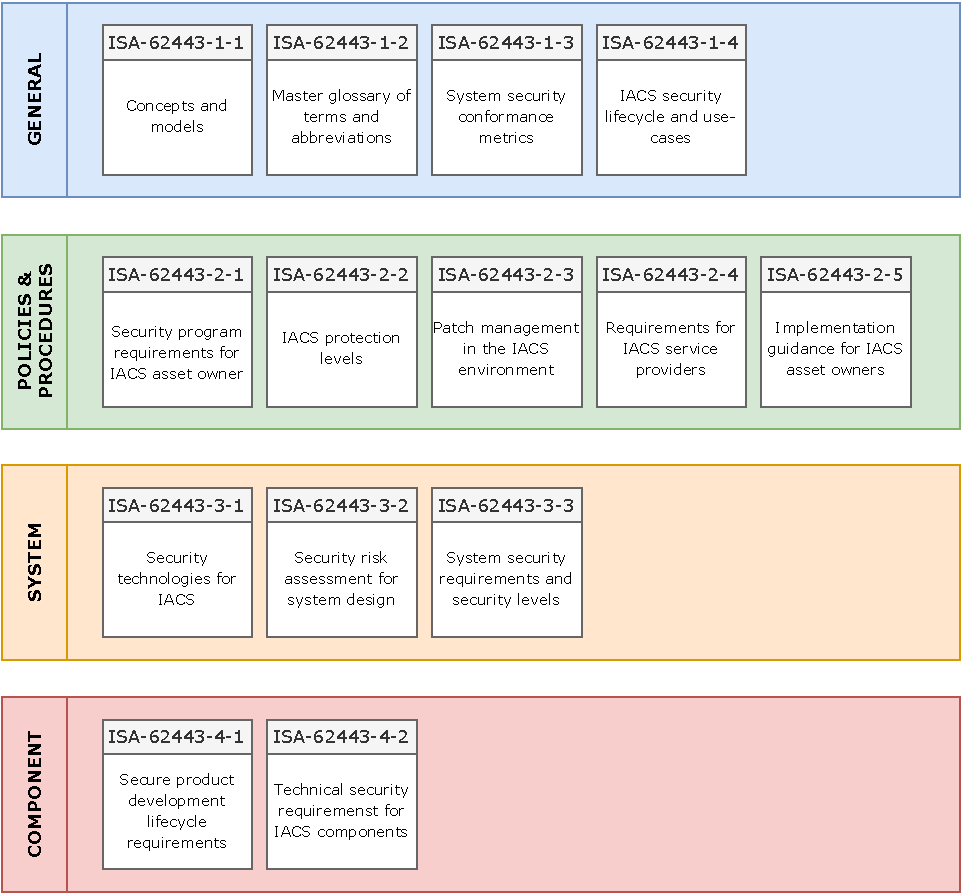
\includegraphics[scale=0.75]{Immagini/ISA_IEC-62443}}
\caption{Schema dei moduli della famiglia ISA/IEC-62443}\label{fig:isa99}

\end{figure}

\begin{figure}[tbh]

\centerline{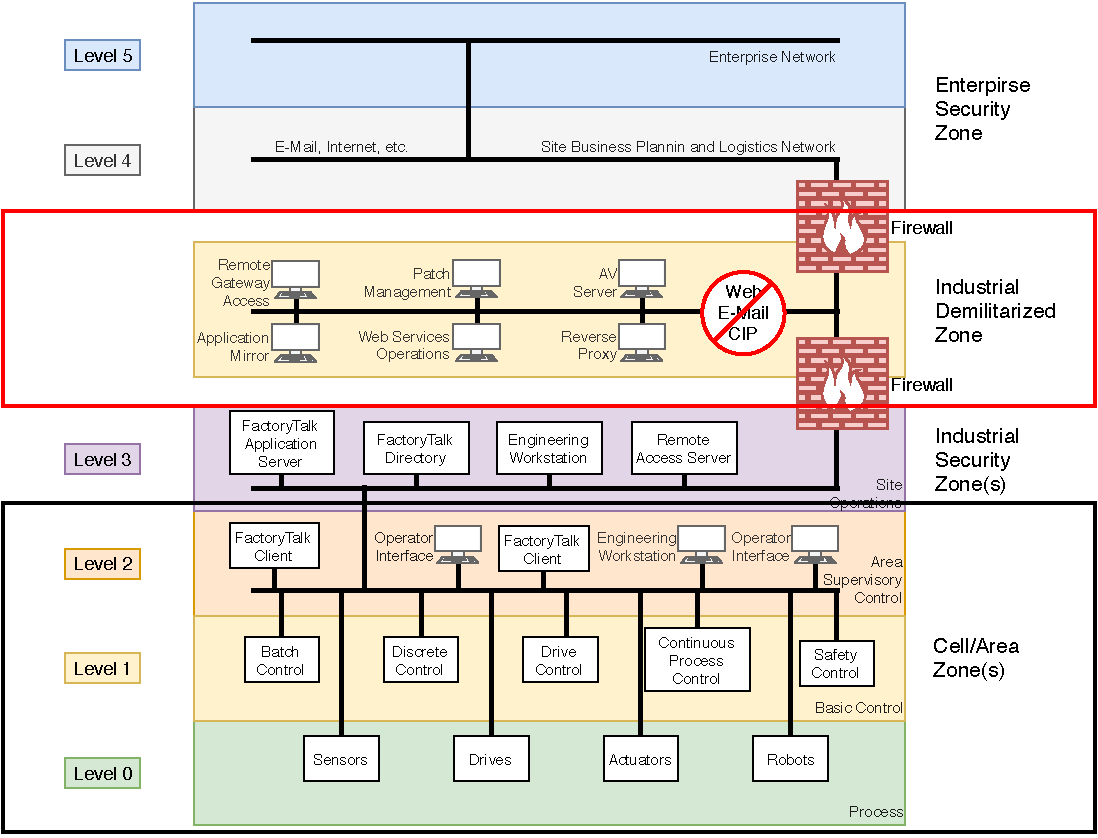
\includegraphics[scale=0.65]{Immagini/pera_model}}
\caption{ Purdue Enterprise Reference Architecture (PERA), modello concettuale per la segmentazione della rete di un ICS}\label{fig:peramodel}

\end{figure}

C'� da sottolineare che l'intero standard ISA/IEC-62443 � sottoposto periodicamente a revisioni ed aggiornamenti, sia nella sua interezza che solamente in alcuni dei suoi moduli. Chiaramente le nozioni basilari restano invariate nel tempo, sono integrate da informazioni aggiornate ed in linea con il progresso tecnologico. � utile quindi vedere quali siano queste nozioni e come si riflettano ad un livello pi� funzionale e pragmatico.

In generale, dai moduli ISA/IEC-62443, si evince l'esistenza di vulnerabilit� comuni a tutti i sistemi di controllo e possono essere sia di natura strumentale che organizzativa. La prima, una delle pi� importanti, � la sottovalutazione delle politiche di sicurezza. Molto spesso si registrano casi di attacchi in cui il motivo primario del problema � stato il mancato rispetto, o addirittura l'assenza, di comuni norme di sicurezza. Questo tema e i problemi che porta con s�, purtroppo, vengono frequentemente trattati come meno importanza di quanto ne richiedano e alle volte non si rileva la presenza neanche degli strumenti organizzativi basilari, quali le documentazioni dei sistemi o delle reti. Anche nel caso in cui siano presenti, spesso non sono aggiornati. Inoltre il monitoraggio delle attivit� di accesso o di registrazione degli incidenti non sono adeguatamente supportate, creando conseguenti difficolt� nel fornire i dati relativi all'affidabilit� della rete e del sistema di controllo. Altri fattori organizzativi critici sono l'assenza di procedure di ``disaster recovery'', backup dei dati o delle configurazioni del sistema e, pi� in generale, piani per la gestione delle emergenze.

Da un punto di vista architetturale, invece, la vulnerabilit� pi� cruciale � la segmentazione e separazione della rete informatica aziendale da quella industriale di controllo del processo (a tale scopo si � cercato di fornire un supporto con il protocollo ISA/IEC-62443 tramite schemi di architetture di riferimento, come il modello PERA rappresentato fig. \ref{fig:peramodel}). Il problema di una rete informatica piatta, ossia non adeguatamente segmentata, � che semplifica estremamente la circolazione di una minaccia al suo interno, per finire con il suo arrivo fino ai PLC. Ci� significa che, in caso di un attacco positivo sapientemente programmato, le conseguenze derivanti potrebbero mettere a rischio la sicurezza non solo degli asset aziendali, ma anche l'incolumit� fisica di oggetti e/o persone ( i PLC, infatti, si trovano a ridosso dei macchinari controllati ed una loro manomissione causerebbe il malfunzionamento dell'intero sistema di produzione).

Altre vulnerabilit� architetturali sono anche fornite dall'assenza o il mancato aggiornamento di comuni software di sicurezza, come antivirus o strumenti di rilevamento dei malware, dettati spesso dall'incompatibilit� tra questi programmi e i software real-time utilizzati nei sistemi di acquisizione dati. Inoltre, capita che i computer su cui operano gli applicativi di controllo non siano correttamente configurati, mantenendo configurazioni standard facilmente attaccabili, o installano sistemi operativi a cui non � stata fatta alcuna operazione di hardening o, per lo meno, di aggiornamento. Infine, altra vulnerabilit� � data dalla mancanza di monitoraggio degli accessi remoti: negli ultimi tempi, infatti, l'utilizzo di dispositivi mobile per gestire questi sistemi si � ampiamente diffuso grazie alla comodit� che li contraddistingue. Questo, per�, ha portato con s� anche numerose criticit� che se non correttamente affrontate possono rappresentare delle vulnerabilit� alla sicurezza del sistema.

\subsection{Differenze tra sicurezza IT e ICS}

Come precedentemente detto, sebbene le tecnologie applicate ai sistemi ICS sia derivante da quella dei sistemi IT domestici, le soluzioni adottate per la sicurezza devono essere differenti a cause delle differenze dovute all'ambiente di lavoro ed alle differenti esigenze. Mentre nel caso della sicurezza IT le propriet� di confidenzialit� e riservatezza dei dati ha maggiore importanza rispetto alla disponibilit�, nei sistema di controllo, data la loro natura operativa continua, � necessario porre la disponibilit� e l'integrit� dei dati in cima alle propriet� da mantenere, anche quando ci si trova sotto attacco. Il rischio, in caso contrario, � di causare gravi perdite economiche o, peggio, danni materiali al sistema o mettere in pericolo l'incolumit� degli operatori del sistema di controllo \cite{Knapp_2015_3}.

Di seguito sar� esposta una lista di differenze, evidenziate anche dal comitato ISA99 al momento dello studio del nuovo protocollo di sicurezza, tra sistemi di sicurezza ICS e quelli IT \cite{Stouffer_2015}.

\begin{description}

\item [Requisiti operativi e temporali]
Di norma, negli ambienti ICS i tempi delle comunicazioni sono fondamentali: devono essere effettuate il pi� possibile in real-time, con le soglie dei livelli di tolleranza dei ritardi e disturbi ammessi dettate dallo scopo a cui sono destinate. In alcuni casi, le risposte del sistema alle interazioni degli operatori sono cos� critiche che si utilizzano sistemi operativi specifici per lo scopo denominati real-time operating system, o RTOS (ovviamente l'unit� di misura per il real-time dipende molto dalle applicazioni a cui � destinato il sistema ed � di norma specificata in fase di progettazione dell'ICS). Molti sistemi effettuano trasmissioni rapide e ripetute, quindi ha molta importanza l'affidabilit� del mezzo di comunicazione, mentre non si rende necessaria una larghezza di banda estesa. Nelle comunicazioni IT, invece, si hanno necessit� diametralmente opposte: il real-time � un'esigenza che pu� essere messa in secondo piani (disturbi e ritardi nelle comunicazioni hanno soglie di tolleranza molto pi� alte), mentre � assolutamente primaria la necessit� di una banda di comunicazione sufficientemente larga per trasportare tutte le comunicazioni del sistema.

\item [Requisiti di disponibilit�]
Molti sistemi ICS, come precedentemente detto, sono in esecuzione ininterrottamente. Interruzioni improvvise del sistema, quindi, non sono accettabili e spesso devono essere pianificati con largo anticipo (giorni o, addirittura, settimane prima). Inoltre � fondamentale effettuare numerosi test intensivi prima di eseguire le operazioni di interruzione,  in modo da garantire la corretta affidabilit� del sistema durante tutto il processo. � quindi facilmente intuibile come le tipiche strategie del mondo IT, quali il riavvio di un componente in caso di malfunzionamenti, non possano essere attuate nell'ambiente ICS, dato l'enorme impatto negativo che avrebbe sulla intero sistema di controllo. Spesso, infatti, � pi� importante mantenere la disponibilit� del processo controllato, rispetto alle informazioni su cui si basa la produzione. A tale scopo, si � gi� visto come in molti ICS l'architettura sia ridondante, per garantirne la funzionalit� anche in caso di componenti non disponibili.

\item [Requisiti di gestione dei rischi]
In un sistema IT, in caso di minaccia andato a segno, le preoccupazioni maggiori sono rivolte all'integrit� e la riservatezza dei dati colpiti dall'attacco. In un ambiente del genere, questi rappresentano l'asset principale ed una loro manomissione si tramuterebbe in gravi danni economici e d'immagine per l'azienda attaccata. In un sistema ICS, invece, le conseguenze sono del tutto imprevedibili e portare alle situazioni pi� disparate: si va dalle perdite di materiali e propriet� intellettuali fino al provocare danni ben pi� gravi che posso mettere a rischio la salute degli operatori o, in caso estremi, della salute pubblica. Quindi, chi si occupa dell'implementazione dei metodi di sicurezza di un impianto ICS deve tenere bene a mente l'importanza del legame esistente tra sicurezza del sistema e sicurezza delle persone. Qualsiasi rimedio che non ne tenga conto � da considerarsi inaccettabile.

\item [Effetti fisici]
Come detto, i PLC interagiscono direttamente e fisicamente con il processo da controllare. Spesso le interazioni possono essere molto complesse e generare dei particolari eventi fisici. Questo rappresenta, ovviamente, un potenziale pericolo che in un ambiente IT non sia ha per niente. Per gestire questi eventi fisici � necessario che gli operatori del sistema di controllo comunichino costantemente con gli esperti del campo fisico in questione.

\item [Sistemi operativi]
I sistemi operativi implementati negli ambienti ICS sono abbastanza differenti dalle loro controparti utilizzate in ambienti IT. E anche qualora si utilizzi un sistema operativo comune al mondo IT (come Windows o Linux), le configurazioni ed i software utilizzati per il controllo sono completamente diverso. Chi deve gestire una rete di un ICS, quindi, deve possedere delle conoscenze e delle capacit� specifiche per quel tipo di ambiente. In caso contrario vorrebbe dire non riconoscere le differenze tra i due ambienti, con il rischio di incappare in gravi conseguenze.

\item [Limitazioni delle risorse]
Molto spesso i sistemi operativi ICS girano su macchine dalle risorse hardware e software limitate, con la conseguenza che alcune delle feature di sicurezza tipiche dei sistemi IT non sono incluse. Caratteristiche come la capacit� di criptare e decriptare dati, log testuale che riporti gli errori o strumenti per la protezione delle password spesso sono assenti dalle macchine di un sistema ICS, sia per questioni hardware che software. E alle volte aggiungere delle nuove componenti aggiornate per implementare le suddette funzionalit� non � una soluzione percorribile, in quanto ne andrebbe della stabilit� dell'intero sistema di controllo.

\item [Comunicazioni]
In un ICS i protocolli di comunicazione utilizzati dai dispositivi periferici, ossia i PLC, sono molto spesso proprietari e messi a disposizione direttamente dalle aziende produttrici. Questo rappresenta un problema, dato che in questo modo si viene a creare un sistema con protocolli misti e da gestire singolarmente in modo da garantire la corretta funzionalit� del sistema. Nei sistemi IT, invece, si fa affidamento a protocolli di comunicazione standard, quali TCP/IP, le cui funzionalit� sono oramai ben conosciute e consolidate.

\item [Gestione degli aggiornamenti]
In generale, sia per gli ambienti IT che per quelli ICS, gli aggiornamenti dei software utilizzati sono importantissimi e ne garantiscono il loro corretto funzionamento. Purtroppo per�, la gestione dell'applicazione di questi aggiornamenti differisce notevolmente quando si prendono in esame i due casi separatamente. Nei sistemi IT, le patch di sicurezza e le migliorie software sono applicate periodicamente e molto spesso in maniera del tutto autonoma, senza richiedere l'intervento di chi opera con la macchina in questione (nelle grandi reti IT aziendali sono presenti dei server adibiti al solo scopo di gestire automaticamente l'aggiornamento di tutte le macchine collegate a quella rete). Nei sistemi ICS, purtroppo, non si pu� eseguire la stessa procedura. Innanzitutto gli aggiornamenti devono essere testati a lungo e in maniera intensiva, sia dai produttori dell'applicazione che dagli operatori del sistemi di controllo, prima di poter essere applicati in maniera definitiva. Inoltre la procedura deve essere pianificata per tempo, in quanto, come visto, l'interruzione improvvisa dell'operativit� del sistema di controllo causerebbe numerosi ed ingenti danni economici all'azienda produttrice. Un altro inconveniente � che spesso i sistemi operativi implementati negli ICS sono obsoleti e non pi� supportati dagli stessi venditori del software. Questo pu� comportare che alcune patch rilasciate non siano compatibili con questi sistemi operativi ed applicarle vorrebbe dire rendere instabile l'intero ICS. Un esempio � stato il caso di Windows XP ed il Service Pack 3 rilasciato da Microsoft che rendeva instabile numerosi sistemi di controllo, tant'� che ad oggi molti di essi ancora utilizzano il Service Pack 2.

\item [Assistenza tecnica]
Tipicamente nei sistemi IT il sistema di assistenza tecnica pu� essere erogato in maniere differenti ed � in grado di gestire tutte le diverse componenti dell'architettura, anche se appartengono a venditori diversi tra loro. Nel caso di un ICS, invece, l'assistenza viene effettuata spesso da parte di una singola azienda e potrebbe applicare delle soluzioni differenti da quelle che applicherebbe un altro venditore. Inoltre, in alcuni casi non � permesso l'utilizzo di soluzioni per la sicurezza messe a disposizione da eventuali terze parti esterne, in quanto impedito dal contratto che l'azienda gestore dell'ICS ha redatto con il venditore delle apparecchiature. Nel caso in cui si venga meno a questa clausola, si rischierebbe di annullare la garanzia offerta dal venditore portando il sistema ad un'esposizione molto pi� diretta a dei potenziali rischi.

\item [Tempo di vita dei componenti]
Nei sistemi IT, le componenti hardware e software hanno una durata garantita per un tempo che va dai 3 ai 5 anni. Questo � dettato dalle rapide e continue evoluzioni tecnologiche, che rendono obsoleti i dispositivi molto velocemente. In un sistema di controllo, invece, si fa largo uso di componenti specificamente studiati per quello scopo. Questo fa s� che la vita di questi strumenti si attesti tra i 10 e i 15 anni, circa il triplo rispetto al caso IT. 

\item [Disposizione fisica dei componenti ]
I sistemi IT sono di norma situati in aree commerciali e facilmente accessibili, per facilitare un eventuale intervento in loco. Questo � il caso anche dei sistemi di controllo situati a ridosso del processo controllato. Le uniche componenti che potrebbero essere situate in luoghi pi� lontani sono i server utilizzati per il backup dei dati. Come abbiamo visto, per�, numerosi ICS, a causa delle caratteristiche geografiche del processo controllato, sono disposti in luoghi molto vasti e raggiungibili solo con mezzi appositi. Inoltre, dato l'alto rischio rappresentato da alcune componenti dei sistemi di controllo , spesso si utilizzano luoghi di installazione pi� isolati proprio per motivi di sicurezza.

\end{description}

In conclusione, � evidente che le differenze operative e di sicurezza di un ICS crei la necessit� di creare delle strategie di sicurezza molto pi� complesse rispetto ad un sistema IT. � necessaria la presenza un team composto sia da operatori di sistemi di controllo che da esperti di sicurezza informatica per individuare e capire le possibili conseguenze dovute alle normali azioni di assistenza: che sia l'installazione di un aggiornamento, operazioni di manutenzione o l'implementazione di una nuova soluzioni per la sicurezza. Tutto ci� deve essere studiato prima di effettuare l'azione in maniera definitiva.

\section{SCADA e dispositivi mobile \label{sec:mobilesecurity}}

\subsection{Applicazioni locali e remote}

Nel corso degli ultimi 2/3 anni si � cominciato a diffondere sempre di pi� anche in ambiente SCADA l'utilizzo di applicazioni su dispositivi mobile per la gestione dei sistemi di controllo.Inoltre, l'idea di affidarsi a piattaforme cloud per svolgere le normali procedure di gestione del sistema, quali monitoraggio degli accessi, attivit� di supervisione e quant'altro, non sembra pi� cos� assurda come poteva apparire qualche anno fa. Tutte queste comodit�, per�, portano ovviamente con loro anche delle criticit� che, se non correttamente risolte, a loro volta potrebbero portare a subire degli attacchi, con annesse perdite economiche.

\begin{figure}[tbh]

\centerline{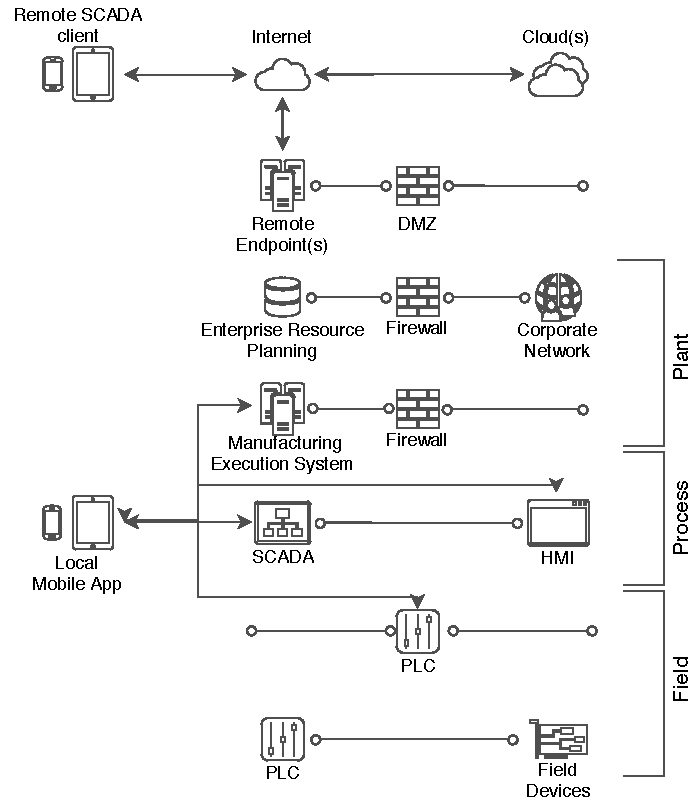
\includegraphics[scale=0.75]{Immagini/scada_mobile.pdf}}
\caption{Architettura di un sistema SCADA integrato con applicazioni mobile}\label{fig:scadamobile}

\end{figure}

L'infrastruttura di un ICS, come precedentemente esposto, pu� essere di natura molto eterogenea, seguendo anche il principio di segmentazione del protocollo ISA99. In figura \ref{fig:scadamobile} � riportato un esempio di architettura di un sistema in cui si fa utilizzo di applicazioni mobile per il monitoraggio e la gestione dell'impianto. Come � possibile notare, i terminali mobile, a seconda del livello dell'architettura in cui sono posti, si possono raggruppare in due categorie:

\begin{description}

\item [Applicazioni locali]
Queste applicazioni sono installate su dispositivi che si interfacciano direttamente con i dispositivi periferici dell'ICS, usualmente tramite connessioni Wifi o Bluetooth. un esempio sono le applicazioni installate su tablet usate dagli ingegneri di controllo per osservare lo stato del processo, anche durante eventuali pause o momenti in cui sono lontani dai terminali fissi. Queste applicazioni posso essere utilizzate anche per altri scopi, come ad esempio configurare le operazioni di un PLC o configurare una schermata HMI, in sostituzione di laptop e pc. In base all'utilizzo, quindi, le applicazioni locali possono essere suddivise a loro volta in:

\begin{itemize}

\item Configuratori di PLC, ossia applicazioni per monitorare, ma anche programmare i vari dispositivi della rete del sistema di controllo, quali PLC, RTU (Remote Terminal Unit, dispositivi elettronici di controllo con cui � possibile monitorare i parametri fisici di un processo e trasmetterli al sistema di elaborazione dell'impianto SCADA) ed altro ancora;

\item Client SCADA, applicazioni tramite cui gli ingegneri di controllo monitorano e supervisiono lo stato del processo. Queste applicazioni si interfacciano con i server SCADA;

\item Pannelli HMI Mobili, ossia delle applicazioni che trasformano il proprio dispositivo mobile in un pannello HMI vero e proprio. Alcuni software mettono a disposizione dei modelli di interfacce con gi� alcune logiche di controllo implementate, ma � possibile, sempre tramite le stesse applicazioni o le loro controparti desktop, creare dei pannelli HMI personalizzati e programmarli a seconda delle proprie esigenze. Una volta create, le interfacce vengono caricati sui server SCADA ed eseguite sui dispositivi mobile, trasformandoli in veri e propri pannelli HMI (i quali possono essere completamente sostituiti, causando anche un notevole risparmio economico).

\end{itemize}

In generale, per quanto riguarda questo tipo di applicazioni, bisogna effettuare alcune considerazioni, basate sul fattore ``ambientale'': queste applicazioni sono utilizzate in un segmento dell'architettura considerato sicuro, in quanto separato tramite firewall dall'esterno. Ci� significa che la mancanza di funzioni per la crittografia dei dati e per svolgere le procedure di autenticazione e autorizzazione non � da considerare come fonte di rischi elevati. Il problema, per�, si pone nell'eventualit� di manomissioni, anche parziali, di queste applicazioni. In questo caso gli attaccanti possono interagire direttamente con il sistema di controllo, influenzando lo stato del processo a proprio piacimento. � chiaro quindi come sia importante che queste applicazioni non vengano utilizzate al di fuori di questi ambienti sicuri, altrimenti il rischio di minacce diverrebbe troppo alto. La conseguenza � che i dispositivi in cui sono installate i software mobile non lasciano mai le stanze di controllo e, soprattutto, non sono connesse con la rete esterna.

\item [Applicazioni remote]
Questo tipo di applicazione permette agli operatori di controllo di connettersi ai server del sistema SCADA tramite canali di comunicazioni remoti, quali rete internet, reti VPN ed altre soluzioni simili. Tipicamente sono utilizzate per eseguire azioni di monitoraggio dei sistemi, ma esistono anche delle applicazioni che permettono di svolgere delle azioni di controllo sul processo. In questo caso sono integrate anche delle funzionalit� di avvertimento tramite degli alert remoti in modo da avvisare l'operatore della necessit� di un suo intervento. 

Confrontandole con le applicazioni locali si pu� subito notare la grossa differenza tra le due categorie: le applicazioni remote utilizzano i vari protocolli Internet per comunicare con il sistema SCADA e spesso sono installate sui dispositivi personali degli operatori. Quindi, l'ambiente in cui operano non pu� essere considerato chiuso e isolato come nel caso delle applicazioni locali. Questo significa che le applicazioni remote sono esposte ad un numero maggiore di rischi ed attacchi provenienti sia dalla rete di comunicazione che da software maligni installati sui dispositivi.

\end{description}

\subsection {Analisi delle vulnerabilit� mobile}

Sebbene le tipologie di applicazioni mobile utilizzate in ambiente SCADA possano essere molteplici, ognuna con le proprie funzionalit�, � possibile stilare una lista di minacce comuni a tutti i suddetti software. Il motivo � da ricercare nelle caratteristiche del mezzo su cui vengono utilizzate: i dispositivi mobile, sebbene molto pratici e comodi, sono di natura molto vulnerabili, non solo agli attacchi software, ma anche a minacce fisiche, come il furto o lo smarrimento. In base al tipo di attacco, quindi, � possibile raggruppare le varie minacce in tre categorie:

\begin{description}

\item [Accesso non autorizzato ai dati]
In questo scenario, l'attaccante riesce ad ottenere l'accesso al dispositivo dove � installata l'applicazione e, di conseguenza, a tutti i dati che sono salvati al suo interno. Pu� avvenire in diversi modi, ma in tutti i casi le conseguenze sono molto gravi.

Uno dei modi che pu� dare il via al suddetto scenario di attacco � la perdita fisica del dispositivo. In questa situazione l'attaccante ha modo di appropriarsi dei dati dell'applicazione sia con attacchi software che hardware. Se il dispositivo � destinato ad un uso locale, l'attaccante otterrebbe delle preziose informazioni riguardo il processo controllato, l'infrastruttura del sistema SCADA, schemi di rete ed altro ancora. Queste informazioni, poi, potranno essere usate per eseguire successivamente un attacco pi� mirato e con pi� alte probabilit� di successo. Nel caso in cui, invece, il dispositivo perso sia destinato ad un uso da remoto, le conseguenze sarebbero ben pi� gravi: gli attaccanti, infatti, potrebbero ottenere tutte le informazioni necessarie per l'autenticazione ed utilizzarle per connettersi direttamente ai server del sistema SCADA.
 
Un altro modo con cui pu� avvenire un accesso non autorizzato � nel caso in cui venga lasciato incustodito un dispositivo mobile senza alcuna protezione. In questo caso l'attaccante ha a disposizione una finestra temporale in cui pu� sia ottenere delle informazioni cruciali, ma anche alterarle senza che nessuno se ne accorga. Similmente, si pu� verificare la stessa situazione quando i dati sono salvati su partizione esterne (tipicamente schede di memoria SD) e queste non vengono protette adeguatamente. Anche in questo caso l'attaccante ha la possibilit� di manipolare e/o accedere ai dati presenti nella partizione senza particolari problemi. 

\item [Compromissione del canale di comunicazione]
Questo scenario ha pi� probabilit� di manifestarsi nel caso delle applicazioni remote, ma ci� non esclude del tutto dal pericolo quelle locali, anch'esse comunque a rischio. Generalmente, il canale di comunicazione che le applicazioni utilizzano per dialogare con i server del sistema SCADA deve garantire il mantenimento delle propriet� di riservatezza ed integrit�. Purtroppo per�, i dispositivi su cui sono installate gli applicativi possono connettersi alla rete Internet attraverso dei canali non sicuri. Questo pu� provocare una serie di pericoli e minacce quali:

\begin{itemize}

\item Connessione ad access point clandestini, sia per reti WiFi che per quelle cellulari;
\item Connessione ad access point pubblici che non integrano funzionalit� per la sicurezza;
\item Compromissione delle rete privata, sia aziendale che domestica;
\item Compromissione della rete VPN.

\end{itemize}

Quale che sia la minaccia, le conseguenze sono sempre le stesse: l'attaccante pu� pianificare un attacco \mitm (sar� esposto pi� nel dettaglio nella sezione \ref{sec:typicalattacks}), ottenendo la possibilit� di osservare il traffico dati in chiaro che ha luogo nel canale di comunicazione in questione. In questa maniera pu� effettuare pu� effettuare lo sniffing delle informazioni scambiate tra server SCADA e applicazione, ma anche manipolarle a proprio piacimento senza essere scoperto.

\item [Compromissione dell'applicazione]
Anche se le applicazioni operano in un ambiente sicuro, con canali di comunicazioni protetti e gli accessi sono controllati, � possibile che vi siano delle vulnerabilit� nel loro codice, esponendole di fatto a pericoli inaspettati. Queste vulnerabilit� del codice possono essere sia dal lato del server (il backend) che nelle applicazioni client. I pericoli che possono scaturire da questo scenario sono diversi, come ad esempio una manomissione delle liste di controllo per gli accessi, l'esecuzione di codice malevolo da remoto o la compromissione di dati riservati.

\end{description}

Basandosi sugli scenari delle minacce appena esposte, si possono individuare due categorie di attacchi mobile ognuno con obiettivi diversi. La prima categoria � formata dagli attacchi il cui scopo � quello di influenzare, in maniera pi� o meno diretta, lo stato del processo controllato. Generalmente pu� avvenire quando l'attaccante ha libero accesso alle credenziali di un operatore e modifica le informazioni cruciali per in controllo di un processo. La seconda tipologia di attacchi � quella che mira ad influenzare le azioni di un operatore SCADA, in modo da fargli compiere delle azioni dannose sul sistema senza che se ne accorga. In questo caso, l'attaccante crea un ambiente di lavoro fittizio, del tutto simile a quello reale, in cui potr� ad esempio cambiare a proprio piacimento i dati sullo stato del processo o scambiare le informazioni da mostrare nei vari pannelli della schermata HMI. Basandosi su queste informazioni alterate, l'operatore si trover� a effettuare in buona fede delle azioni di controllo, ma che in realt� finiranno per danneggiare il sistema SCADA ed il processo controllato.

La sicurezza dei dispositivi mobili, inizialmente sottovalutata, � tornata sotto i riflettori negli ultimi anni. Numerosi sono i stati i lavori di studio effettuati per attirare l'attenzione sui problemi nascosti in questi software che hanno sicuramente reso l'ambiente degli ICS di pi� facile utilizzo, ma al contempo pi� vulnerabile. Un lavoro dettagliato in questo senso � quello svolto dagli esperti di sicurezza informatica Alexander Bolshev e Ivan Yushkevich. I due esperti, basandosi sulla classificazione delle applicazioni e delle minacce precedentemente fornita, nel corso degli anni hanno analizzato nel dettaglio le applicazioni per mobile presenti sul mercato. I dati ottenuti sono poi stati esposti in rapporti tecnici dettagliati. Nel loro ultimo lavoro \cite{Bolshev_2018}, pubblicato nel gennaio dello scorso anno, hanno analizzato software creati da oltre 30 venditori. In queste hanno riscontrato un totale di 147 falle della sicurezza , ognuna delle quali � stata categorizzata seguendo le linee guida fornite dal ``Open Web Application Security Project'' (OWASP), un ente no-profit istituito nel 2001 con lo scopo di aiutare a migliorare la sicurezza dei software. L'OWASP prevede un totale di 10 categorie per i rischi delle applicazioni mobile:

\begin{itemize}

\item \textbf{utilizzo improprio della piattaforma}, ossia l'uso improprio o il mancato impiego delle funzionalit� di sicurezza messe a disposizione dello sviluppatore;
\item \textbf{archiviazione impropria dei dati}, che ricopre l'errata gestione dei dati utilizzati dall'applicazione;
\item \textbf{comunicazione non sicura}, in cui rientrano tutti i problemi nel creare un canale di comunicazione adeguato;
\item \textbf{autenticazione non sicura}, ossia vulnerabilit� dovute alla errata gestione della sessione o all'autenticazione dell'end user;
\item \textbf{crittografia insufficiente}, che include problemi dovuti ai tentativi di crittografia errati;
\item \textbf{autorizzazione non sicura}, in cui sono compresi i tentativi errati nel gestire le autorizzazioni;
\item \textbf{qualit� del codice client}, che raggruppa gli errori di codice presenti nell'applicazione;
\item \textbf{manomissione del codice}, ossia i problemi dovuti alle modifiche che � possibile apportare al codice dell'applicazione una volta installata;
\item \textbf{reverse engineering}, che identifica la capacit� di ottenere il codice sorgente partendo dal software;
\item \textbf{funzionalit� non pertinenti,} ossia funzionalit� aggiuntive utilizzate in fase di sviluppo erroneamente mantenute nell'applicazione finale.

\end{itemize}

A queste categoria ne hanno aggiunta una specifica per l'ambiente di lavoro SCADA, ossia \textbf{errori presenti nella programmazione del codice implementato nel backend}.

%tabella categorie mobile
\begin{table}[tbh]
\begin{tabularx}{\textwidth}[c]{@{}XlXl@{}}
\toprule
\textbf{OWASP ID} & \textbf{Categoria OWASP}                      &\textbf{ N� di errori} & \textbf{\% di Applicazioni} \\ \midrule
M1       & Utilizzo Improprio della Piattaforma & 5                & 6\%                \\
M2       & Archiviazione Impropria dei Dati     & 20               & 47\%               \\
M3       & Comunicazione Non Sicura             & 11               & 38\%               \\
M4       & Autenticazione Non Sicura            & 6                & 18\%               \\
M5       & Crittografia Insufficiente            & 8                & 24\%               \\
M6       & Autorizzazione Non Sicura            & 20               & 59\%               \\
M7       & Qualit� del Codice Client            & 12               & 35\%               \\
M8       & Manomissione del Codice              & 32               & 94\%               \\
M9       & Reverse Engineering                  & 18               & 53\%               \\
M10      & Funzionalit� Non Pertinenti          & 8                & 24\%               \\
         & Errori Lato Backend                  & 7                & 12\%               \\ \bottomrule
\end{tabularx}
\caption{Statistiche vulnerabilit� applicazioni SCADA per mobile \cite{Bolshev_2018}.}
\label{tab:bolshev_table}
\end{table}

Nella tabella \ref{tab:bolshev_table} sono riportati i risultati dell'analisi effettuata dai due studiosi. � possibile notare come qualche categoria presenti una bassa percentuale di errori, mentre alte sono moto elevate. Da notare come la categoria inerente alla manomissione del codice abbia una percentuale molto elevata, segno che alcuni problemi spesso sono ancora sottovalutati.

\section{Scenari di attacco \label{sec:typicalattacks}}

Esistono molti metodi per attaccare un obiettivo, una volta che questa � stato identificato. I vari attacchi usati in ambiente, \mitm, \dos, attacchi replay, phishing, infezione dei sistemi con malware, sono molto efficaci anche in ambiente ICS. I motivi primari, come visto nei precedenti paragrafi, sono da ricercarsi in una combinazione di fattori legati a protocolli di comunicazione non sicuri, autenticazione tra dispositivi molto scarna e architetture di rete fragili.

 Se una rete venisse penetrata ed installato un malware al suo interno, tramite dei tool specifici si potrebbe garantire l'accesso remoto al sistema, installare dei keylogger o intraprendere qualsiasi altra azione distruttiva. In alcuni casi le informazioni possono essere estrapolate ed utilizzate per effettuare un ulteriore attacco. Inoltre, se un attacco riesce ad andare a segno senza lasciare alcuna traccia, l'attaccante pu� rimanere all'interno del sistema indefinitamente. Nel caso in cui ci� accada nella rete di un sistema collegato ad altri sistema (come pu� essere una rete di un server di una stanza di controllo SCADA), a questo punto si ha la possibilit� di iniziare un ulteriore attacco con obiettivo altre parti della rete industriale, aumentando l'ammontare dei danni provocati.

Di seguito verranno esposti i tipi di attacchi informatici pi� comuni che possono essere effettuati, le modalit� in cui essi si svolgono e quali difese possono essere implementate nell'architettura di un ICS per contrastarli \cite{Knapp_2015_7} \cite{Stouffer_2015}.

\subsection{Attacco \mitm}

Con \mitm (abbreviato in \mitma) ci si riferisce ad un attacco in cui l'attaccante riesce a frapporsi fra due dispositivi in comunicazione senza che se ne accorgano, riuscendo in questo modo a catturare tutti i dati e le informazioni scambiate durante il dialogo. L'attaccante, per fare ci�, si connette ad entrambi i dispositivi ed inizia a gestire tutto il traffico dati tra di loro in modo da far sembrare che stiano comunicando direttamente tra loro, quando in realt� la comunicazione si sta sviluppando attraverso un terzo dispositivo in ascolto.

Al fine di eseguire un attacco \mitma, l'attaccante deve essere in grado di intercettare i traffico tra i due obiettivi. Se la connessione da attaccare risulta mancante di funzionalit� per la criptazione dei dati e l'autenticazione dei dispositivi connessi, come spesso accade nei protocolli di comunicazione industriali, il procedimento � molto diretto e veloce. Ma, anche nel caso in cui queste funzionalit� siano presenti, � comunque possibile effettuare un attacco, ad esempio intercettando lo scambio delle chiavi di autenticazione e sostituirle con delle copie personali.

Un altro metodo per effettuare un attacco \mitma � quello di agire sulle tabelle di risoluzione degli indirizzi e modificarle per ottenere l'accesso al flusso delle informazioni scambiate. Questo pu� essere fatto sia nelle tabelle del Address Resolution Protocol (ARP), effettuando un attacco di tipo ARP Poisoning, che in quelle del Domain Name System (DNS), dando luogo in questo caso ad un attacco DNS Poisoning. Prima di mostrare le modalit� con cui si svolgono i due attacchi, � bene effettuare una panoramica sulle funzionalit� per cui sono utilizzati i protocolli ARP e DNS. 

L'ARP � un protocollo di servizio, incluso nel protocollo IP, che agisce a livello di accesso alla rete ed il cui compito � quello di effettuare una mappatura tra indirizzi IP e indirizzi MAC dei dispositivi connessi alla rete locale. Il DNS, invece, � un sistema di indirizzamento, presente sempre nel protocollo IP, che agisce a livello applicazione ed � utilizzato per tradurre il nome di un nodo della rete o host in un indirizzo IP. Iin entrambi i casi, per velocizzare le operazioni di traduzione, si fa utilizzo di tabelle di cache, solitamente memorizzate all'interno dei server aziendali. Queste tabelle sono l'obiettivo degli attacchi ARP Poisoning e DNS Poisoning: ad un attaccante baster� modificare opportunamente i valori delle cache inserendo quelli del proprio indirizzo IP o MAC, a seconda che si agisca rispettivamente sulla cache di un server DNS o di uno ARP, in modo da riuscire ad instradare tutto il traffico verso la propria macchina senza che gli interlocutori se ne accorgano.

Una volta che l'attaccante � riuscito ad intromettersi nel flusso delle informazioni, avr� il completo controllo sulle stesse dando l'inizio all'attacco vero e proprio. Uno scenario tipico � quello di un attacco replay in cui l'attaccante, una volta intercettate le informazioni ricevute dal pannello HMI, le modifica per far compiere al dispositivo di controllo delle azioni dannose. Nel frattempo, i dati inizialmente catturati vengono ritrasmessi al pannello HMI, in modo da non far accorgere l'operatore di nulla. Esiste un altro modo per effettuare un attacco replay, complementare a quello appena esposto e prevede che sia l'operatore stesso ad effettuare delle azioni dannose per il sistema. In questo caso, l'attaccante modificher� i dati da trasmettere al pannello HMI, in modo da indicare la presenza di un problema nell'impianto. L'operatore, quindi, inizier� al routine di correzione del problema, causando per� degli eventi dannosi e imprevedibili.

Esistono dei metodi da applicare con cui potersi difendere dagli attacchi \mitma o, in generale, che permettono la mitigazione degli effetti negativi. Oltre, ovviamente, ad utilizzare tecniche di cifratura e autenticazione robuste(o comunque implementarne di migliori laddove gi� esistano), in modo da creare un ostacolo difficile da superare per gli attaccanti, nel caso in cui l'attaccante faccia uso di metodi di ARP Poisoning o DNS Poisoning vi sono delle ulteriori soluzioni.

Per contrastare in partenza un attacco ARP Poisoning si possono utilizzare diversi metodi, i pi� comuni sono quelli del MAC Address Locking (o port security) e delle tabelle di indirizzamento statiche. Con il primo metodo si va a creare un'associazione univoca tra un indirizzo MAC ed una specifica porta dello switch di comunicazione. Se l'indirizzo MAC della macchina connessa alla porta non combacia con quella associata, la comunicazione viene interrotta e l'intruso non potr� pi� raggiungere il suo obiettivo. Inoltre con questo metodo si garantisce un livello di protezione fisica ulteriore, in quanto pu� impedire l'utilizzo di macchine non aggiornate e pi� vulnerabili all'interno di una rete protetta. Il secondo metodo si basa sul presupposto che la rete informatica di un ICS non subisce grosse variazioni di composizione e pu� essere considerata relativamente statica. Partendo da ci� � possibile codificare gli indirizzi MAC in maniera statica nelle tabelle ARP presenti in ogni computer, cosicch� si impedisca all'attaccante di cambiarne i valori. Chiaramente questa tecnica diventa difficile da implementare quando ci si trova nel caso di reti molto estese e/o caratterizzata da un elevato dinamismo delle macchine connesse.

Anche nel caso di DNS Poisoning esistono metodi di prevenzione e mitigazione. Il primo ed il pi� efficace � quello di utilizzare il protocollo DNSSEC (Domain Name System Security Extensions). Questo prevede l'utilizzo di una firma crittografata per ogni record inserito nelle tabelle di cache che sar� utilizzata dal DNS resolver per verificare l'integrit� e l'autenticit� dei dati ricevuti. Se cos� non fosse, i dati verrebbero scartati a priori e sarebbe lanciato un messaggio d'errore all'operatore. Ulteriori metodi prevedono l'utilizzo di tecniche di validazione end-to-end a livello di trasporto una volta stabilita la connessione tra i due dispositivi. Ad esempio, utilizzando il protocollo HTTPS, � possibile controllare che il certificato digitale del server sia valida ed appartenga al legittimo proprietario.

Infine � consigliabile l'uso di programmi adibiti all'individuazione di questi attacchi. Questi software agiscono ispezionando i dati prima che questi vengano trasmessi: se questi sembrano essere stati manipolati, il programma blocca la trasmissione dei dati ed avverte l'operatore della presenza di un tentativo di attacco.

\subsection{Attacco \dos}

Si ha un attacco \dos (\dosa) quando si scatena un evento malevolo con l'intento di rendere una risorsa non pi� disponibile all'utente. Come si pu� immaginare, � una categoria molto vasta ed eterogenea che pu� includere qualsiasi tipo di indisponibilit�, dalla perdita di comunicazione con un dispositivo fino all'inibizione o manomissione di particolari funzionalit� del sistema di controllo, come l'archiviazione, l'elaborazione continua ed altro ancora. Un attacco\dosa prevede l'utilizzo, da parte dell'attaccante, di una singola macchina con cui inviare un grossa quantit� di richieste da elaborare al sistema da attaccare. Per amplificare gli effetti di questo attacco e diminuire i tempi di esecuzione, ne � stata concepita una versione che agisce su larga scala, denominato \ddos (\ddosa). In questo caso, l'attaccante sfrutta una rete di macchine, creata appositamente per lo scopo e chiamata ``botnet'', per attaccare il sistema vittima da pi� nodi di comunicazione. In questo caso l'attaccante avr� l'ulteriore possibilit� di nascondere la propria identit� in maniera pi� efficace, poich�, una volta inviato il segnale di attacco alla botnet, potr� scollegarsi dalla rete e far sparire le proprie traccie, mentre l'attacco verr� svolta in maniera completamente autonoma. A parte la differenza dovuta ai tempi di esecuzione dell'intera operazione, gli effetti di un attacco \ddosa sono pressoch� gli stessi di un attacco \dos. Per brevit�, quindi, in questo paragrafo si parler� solo di attacchi \dos, ma il discorso si estende anche a quelli \ddos.

Normalmente gli attacchi \dosa rivolti contro i tradizionali sistemi IT non hanno un cos� forte impatto economico negativo, se ovviamente sono presi e gestiti per tempo. Alcune tra le pi� comuni conseguenze possono essere rallentamenti nell'accesso ad una pagina web o nella gestione delle e-mail, ma alla risoluzione del problema le normali funzionalit� vengono ripristinate. In questi sistemi raramente l'interruzione dei servizi porta al verificarsi di conseguenze fisiche, ma ci� non toglie che un attacco \dosa ben strutturato possa causare lo spegnimento delle diverse macchine collegate alla rete informatica presa di mira.

In uni sistema SCADA, invece, le conseguenze possono essere ben pi� gravi, come ad esempio nel caso in cui l'obiettivo dell'attacco sia un ICS automatizzato, che opera in maniera continua e controlla un determinato processo fisico (il flusso di un liquido in una conduttura di distribuzione, la produzione di energia elettrica, la produzione di parti meccaniche, ecc.) tramite dei controller hardware e software. L'impossibilit� di uno dei controller, a seguito di un attacco \dosa, di eseguire la normale routine di azioni programmate, � denominata ``Loss of Controll (LoC)'' e pu� portare ad interrompere istantaneamente l'operativit� del sistema di controllo mentre il processo viene messo in uno stato di sicurezza (ossia avviene lo spegnimento dell'impianto). Ci� chiaramente rappresenta un pericolo da evitare assolutamente perch�, come detto in precedenza, quando un sistema SCADA cessa improvvisamente di funzionare, le conseguenze che ne scaturiscono possono essere molto gravi e portare anche a gravi danni fisici e ambientali.

Allo stesso modo, nel caso in cui l'obiettivo dell'attacco \dosa sia una scherma HMI, anche se questa non � direttamente connessa con il sistema di controllo meccanico, le conseguenze che ne possono scaturire non sono di certo meno gravi. Tipicamente in questo scenario l'attaccante rivolge i propri sforzi cercando di bloccare il sistema di autenticazione remoto, o RADIUS (Remote Authentication Dial In User Service). In questa maniera l'operatore viene espulso dalla rete e non pu� pi� monitorare lo stato del processo controllato. Questa situazione, analogamente al caso precedente, � denominata ``Loss of View (LoV)'' e, se non si riesce ristabilire il contatto in tempi brevi, l'univo modo per contrastarla � un riavvio dell'intero sistema di controllo, con le solite conseguenze viste dal grave impatto negativo.

Per contrastare questa tipologia di attacchi, purtroppo non esistono dei metodi definitivi, ma piuttosto una serie di rimedi, accortezze e linee guida da seguire per mitigare le conseguenze negative. Innanzitutto � molto importante prendere consapevolezza dei rischi a cui si � esposti quando si subisce un attacco \dosa ed organizzare le risorse su cui si fa affidamento pi� spesso in modo da ridurre l'impatto negativo che l'attacco stesso pu� avere su di esse. Inoltre � molto importante conoscere i servizi messi a disposizione dal proprio provider di servizi internet (ISP) per contrastare un attacco \dosa, come ad esempio il cambio degli indirizzi IP della propria rete o il blocco di quelli da cui proviene l'attacco.

A livello funzionale, invece, si pu� agire sul proprio sistema sovradimensionandolo rispetto alle normali esigenze operative. In questo modo si rende il sistema in grado di sopportare pi� a lungo un attacco \dosa mentre si cerca di identificare la sorgente o comunque prepararlo per lo spegnimento senza causare gravi danni all'impianto di controllo. Un ulteriore metodo operativo per contrastare questi attacchi � quello di utilizzare meccanismi di controllo e osservazione del traffico dati sulla rete in modo da individuare quando � in atto un attacco \dosa o \ddosa. Un esempio � quello fornito in \cite{Genge_2015} che sfrutta le tecnologie ``Software-defined networking (SDN)''. Questa rappresenta un nuovo approccio con cui si cerca di integrare il cloud computing nell'architettura di una rete, separando le funzioni di forwarding e di routing dei pacchetti di rete. 

L'esempio fornito da B{\'{e}}la Genge in \cite{Genge_2015} prevede la presenza di un controller SDN che fornisce continuamente informazioni sul traffico dati ad un'applicazione di monitoraggio. Questa, allo stesso tempo, dialoga con il controller fornendogli aggiornamenti sullo stato della rete. Non appena viene individuato l'inizio di un attacco \dos, il controller SDN viene informato e subito devia il flusso di dati incriminato in modo da proteggere la rete del sistema di controllo

\subsection{Attacchi Phishing}

Nonostante il progresso tecnologico abbia portato alla creazione di metodi di attacco sempre pi� complesse e difficile da contrastare, spesso le pi� efficaci risultano essere quelle legate a tecniche di social engineering. La loro caratteristica principale � l'utilizzo di metodi a bassa tecnologia per coinvolgere la vittima nell'azione d'attacco, senza che questa se ne renda conto. 

Da recenti ricerche svolte sugli attacchi informatici subiti dalle aziende emerge che pi� del 90\% di essi ha avuto inizio per mezzo di tecniche di phishing \cite{Widup_2018}. Questa � una delle tecniche preferite dagli hacker per creare delle minacce di tipo ``Advanced Persistent Threat (APT)'', ossia un attacco con cui si ottiene l'accesso non autorizzato nella rete informatica della vittima, rimanendo nascosti per un lungo periodo di tempo. 

Esistono numerosi versioni di attacchi phishing, ma tipicamente la metodologia rimane sempre la stessa: viene inviata una mail alla vittima con cui si cerca di convincerla a fornire dati sensibili con l'inganno, ad esempio facendo compilare loro dei finti questionari, o, installare dei software malevoli, spesso inviati sotto forma di documenti allegati al messaggio, con cui si ottiene accesso alla rete della vittima. Una volta guadagnato l'accesso, si d� inizio all'attacco vero e proprio. Nel contesto industriale la tipologia di phishing che � utilizzata pi� spesso � lo spear phising, consistente nell'includere nel messaggio i dati personali della vittima, rivolgendosi a lui con nome, cognome, titolo ed altre informazioni private, in modo da aumentarne la credibilit� ed avere pi� probabilit� che venga letto. Tipicamente gli obiettivi a cui sono rivolti i messaggi di spear phishing sono persone che ricoprono incarichi particolari, in quanto spesso in possesso di informazioni cruciali per l'azienda.

Essendo basati su tecniche di social engineering, non esistono dei rimedi assoluti agli attacchi di phishing. L'arma pi� potente a disposizione � sicuramente quella di instillare nel personale della compagnia una cultura di consapevolezza dei pericoli: un dipendente deve essere in grado di distinguere quali sono i messaggi ricevuti legittimi e quali, invece, nascondono dei tentativi di intrusione. Inoltre non deve mai condividere informazioni riservate e/o personali, a meno che l'interlocutore non sia affidabile e la sua identit� sia gi� stata confermata. Sempre riguardo i dati, � consigliabile che anche quelli meno sensibili, come appunto nome, cognome e indirizzi e-mail, non vengano divulgati con troppa facilit�. Nella maggior parte dei casi, infatti, gli attaccanti riescono a personalizzare i messaggi di spear phishing con informazioni facilmente reperibili sul web.

 Ma la sola consapevolezza, spesso, non � sufficiente come arma. Ecco perch� � sempre consigliabile fare utilizzo di programmi per bloccare i tentativi di attacco di phishing. Usualmente questi software scansioni tutti i messaggi sospetti in entrata alla ricerca di una serie di parametri che mostrino l'eventuale natura malevola dell'email. Altre azioni eseguite da questi programmi sono la scansione sia di eventuali URL inclusi nei messaggi che di file allegati, eliminandoli nel caso in cui risultino infetti.
 
\subsection{Attacchi con software malevoli (malware e worm)}
 
Come detto nei precedenti paragrafi, molto spesso alcune tecniche sono utilizzate per predisporre tutti gli strumenti a disposizione prima di effettuare l'attacco vero e proprio. Questi strumenti molto spesso sono programmi appositamente creati per svolgere dei compiti specifici e in alcuni casi possono riprodursi anche in maniera autonoma all'interno della rete attaccata, in modo da diffondersi su pi� macchine possibili ed amplificare l'effetto distruttivo per cui sono stati creati. 

I software utilizzati pi� frequentemente per questi scopi sono malware e worm, termini spesso usati come sinonimi ma che in realt� identificano due tipologie di programmi diverse tra di loro. Un malware, termine abbreviativo per ``malicious software'' (letteralmente ``programma malintenzionato''), � una qualsiasi programma utilizzato per disturbare le normali operazioni svolte al computer, rubare informazioni o permettere di accedere al sistema senza autorizzazione. In un sistema SCADA i malware possono essere utilizzati in diverse maniere: se installato in una macchina HMI, posso cominciare a generare istruzioni sbagliate da far svolgere al sistema SCADA, provocando malfunzionamenti e errori nel sistema di controllo. Un altro utilizzo � quello di agire come \mitm, occupandosi del dirottamento dei messaggi in modo che siano inviati alla macchina dell'attaccante. Inoltre esistono numerosi malware utilizzati come keylogger, ossia programmi che registrano qualsiasi cosa venga digitata sulla tastiera del dispositivo, come backdoor, tramite cui � possibile avere un punto di accesso al sistema non autorizzato, ed altro ancora.

I worm sono una particolare categoria di malware, il cui tratto distintivo � la capacit� di auto replicarsi su tutte le macchine in cui riesce a diffondersi. Spesso viene erroneamente identificato come virus, ossia un malware che sfrutta lo scambio di file tra computer per potersi diffondere il pi� possibile. Un worm, invece, sfrutta le connessioni di una rete per potersi riprodurre su tutti i sistemi collegati ad essa. Questo rappresenta un grosso vantaggio per l'attaccante dato che, tipicamente,  in un sistema SCADA, il passaggio di file tra computer � molto limitato. Al contrario, esistono moltissime connessioni tra i dispositivi di un impianto di controllo e ci� permette ad un worm di arrivare a colpire direttamente i PLC, andando ad influenzare in maniera attiva il controllo di un processo.

L'infezione iniziale pu� avvenire in modi diversi: come visto gli attacchi di phishing possono essere uno dei vettori utilizzati per penetrare all'interno del sistema, ma non � da escludere che tutto possa partire da un semplice dispositivo di archiviazione esterno, come una chiavetta USB o una scheda di memoria SD. Al momento dell'inserimento in una macchina, il worm si attiva, viene installato in maniera silenziosa nel computer e inizia la sua attivit�, cercando contemporaneamente di riprodursi su altre macchine collegate a quella che lo ospita.

Worm e malware rappresentano delle minacce molto pericolose. Pi� di un volta sono stati registrati casi in cui, a causa di essi, sono stati riportati danni molto seri ad impianti di controllo. Fra tutti, i pi� diffusi sono sicuramente il worm Stuxnet ed il malware Dragonfly, i cui metodi operativi verranno esposti pi� in dettaglio nella sezione \ref{sec:malwarecasestudy}.

Anche in questo caso non esistono dei metodi di difesa efficaci al 100\%: spesso questi programmi sfruttando bug dei sistemi operativi che non sono ancora stati segnalati o di cui ancora non � disponibile un patch per la correzione. Per prevenire una loro intrusione, quindi, occorre come sempre accortezza da parte degli operatori: controllare sempre i file che si sta per utilizzare, in modo da accertarsi della loro integrit�. Inoltre, se � necessario fare uso di dispositivi rimovibili, evitare che questi vengano esposti all'ambiente esterno. Ovviamente, come nei casi precedenti, esistono programmi anti-malware che permettono l'individuazione e l'eliminazione nelle macchine di software dannoso, ma hanno dei lati negativi:

\begin{itemize}

\item per individuare il software � necessario eseguire una scansione che analizzi tutti i file presenti in una macchina, andando per� ad impattare inevitabilmente sulle prestazione della stessa;

\item se il malware viene programmata basandosi su una vulnerabilit� al ``zero-day'', ossia che non � ancora stata scoperta, il software anti-malware non riuscir� ad intervenire, in quanto incapace di riconoscere la minaccia.

\end{itemize}
 
\subsection{Attacchi combinati}

Molti dei pi� grandi attacchi effettuati ai danni di un ICS non utilizza un'unica vulnerabilit� presente su un unico obiettivo, ma, al contrario sono attacchi altamente sofisticati che combinano elementi di diversi tipi di malware, utilizzando molteplici vettori d'attacco, in modo da aumentare la gravit� del danno causato e la velocit� con cui il software riesce a diffondersi. 

Originariamente gli attacchi combinati utilizzavano diverse tipologie di malware, il cui dispiego avveniva in maniera sequenziale. Un esempio pu� essere un attacco phishing con cui si ottiene l'accesso nel sistema, scavalcando il firewall. Da qui poi viene avviato un keylogger, con cui si acquisiscono le credenziali di accesso alla rete interna, rendendo possibile un attacco diretto al sistema di controllo o ottenere dati importanti e protetti. Al giorno d'oggi, il concetto di attacco combinato si � evoluto fino ad arrivare ad un grado di complessit� veramente elevato. Il primo caso fu proprio registrato con Stuxnet (\ref{sec:stuxnet}), un worm in grado di variare il suo comportamento a seconda dell'ambiente in cui veniva eseguito. Questo concetto � stato chiaramente portato avanti, sfociando nella creazione di altri malware molto pericolosi e altrettanto complessi, come ad esempio Flame, una delle numerose varianti create a partire dallo steso Stuxnet.

Alla fine di questo capitolo � stata riportata una tabella in cui sono specificati diversi tipi di attacchi, a seconda del dispositivo o sottosistema che si intende attaccare (\ref{tab:threat_table}).

\section{Case study: il worm Stuxnet ed il malware Dragonfly \label{sec:malwarecasestudy}}

Gli attacchi informatici diretti alle reti di sistemi ICS, fino a una decina di anni fa, era puramente teorici. Il primo caso di un malware creato per danneggiare un sistema SCADA � stato documentato nel 2010, quando venne scoperto per la prima volta il worm Stuxnet.  A distanza di quattro anni � stata resa nota l'esistenza di un'altra minaccia molto sofisticata che colpiva il mondo ICS, Dargonfly, un malware utilizzato per scopi di spionaggio. Ovviamente, si sono succeduti molti altri attacchi nel corso degli anni successivi, molti dei quali sfruttavano il paradigma operativo che era stato implementato per lo stesso Stuxnet. Si possono citare, come esempio, Shamoon e Flame (quest'ultimo conosciuto anche come Flamer o Skywiper), due worm creati a partire da alcune delle vulnerabilit� portate alla luce con Stuxnet. 

In questa sezione sono presi come case study Stuxnet e Dragonfly, in quanto considerati tutt'ora i due software che gettato le basi per tutti i successivi attacchi creati nel corso degli anni.

\subsection{Stuxnet\label{sec:stuxnet}}

Secondo molti esperti di sicurezza informatica, Stuxnet � uno dei malware pi� sofisticati attualmente esistente \cite{Zetter_2015}. Si pensa, nonostante non vi sia mai stata una conferma da parte degli organi interessati, che abbiano contribuito alla sua creazione un tema americano dell'NSA, in collaborazione con un team della corrispettiva agenzia di sicurezza nazionale israeliana \cite{Sanger_2012}.

Il worm fu scoperto nel giugno del 2010 in un impianto nucleare situato a Natanz, in Iran, per merito di alcuni ispettori dell'International Atomic Energy Agency (IAEA). Questi si accorsero, mentre osservavano dei filmati dell'impianto di sorveglianza, che i tecnici dell'impianto avevano sostituito un gran numero di centrifughe per il trattamento dell'uranio, in seguito a dei malfunzionamenti. Sebbene all'inizio la cosa fu vista come normale prassi (non � raro che queste componenti si guastino con il passare degli anni), quello che fece scattare il campanello d'allarme fu la cadenza con cui si verificavano i malfunzionamenti, molto elevata, e l'ulteriore fatto che lo stesso rateo con cui avvenivano i guasti incrementasse con il passare del tempo. Inizialmente gli esperti erano molto fiduciosi sui sistemi di sicurezza implementati nella centrale ed esclusero l'idea di un attacco hacker (la rete informatica della centrale nucleare era completamente isolata dall'esterno, era impossibile accedervi via Web). Ma alla fine, dopo una serie di indagini, si cap� che il malfunzionamenti non erano dovuti n� a fattori fisici dovuti a componenti mal progettati, n� all'errore umano degli operatori, ma erano tutti imputabili alla presenza di un software malevolo nel sistema, ossia Stuxnet, che agiva infettando l'hardware delle centrifughe. L'inizio della propagazione, molto probabilmente, � da imputare ad una chiavetta USB infetta che, una volta connesso ad uno dei terminali SCADA diede inizio a tutto l'attacco.

Stuxnet, originariamente, � stato creato basandosi su quattro vulnerabilit� al zero-day, rendendolo capace di infettare macchine con sistema operativo Windows di diverse generazione: da Windows 2000 fino a Windows 7/Server 2008R2. L'obiettivo primario della sua programmazione � quello di compromettere il software HMI della Siemens (l'azienda produttrice dei PLC utilizzati per controllare le centrifughe della centrale iraniana) WinCC e PCS7, cos� come compromettere degli specifici modelli PLC S7, sfruttando il bus di comunicazione Profibus. 

Tenendo a mente l'obiettivo principale, le azioni che Stuxnet poteva intraprendere variavao in base ai software installati nel sistema che lo ospita. Se all'interno della macchina infettata non era presente nessuno dei programmi obiettivi, allora veniva installato un rootkit, ossia una collezione di software, affinch� il malware venisse eseguito silenziosamente ad ogni avvio della macchina. Dopodich� iniziava ad applicare i metodi per cercare di propagarsi su altre macchine, sfruttando fino a sette differenti mezzi. Addirittura, per quelli che sfruttavano l'utilizzo di un dispositivo USB rimovibile, il worm aveva implementato un protocollo tramite cui si cancellava una volta che il dispositivo USB aveva infettato tre nuovi sistemi. Una volta installato in una macchina in cui era presente il software obiettivo, Stuxnet iniziava l'esecuzione di un'altra serie di metodi con cui riusciva ad installarsi nel database di WinCC o, addirittura, copiarsi nei file dei progetti utilizzati per programmare i PLC S7. Inoltre poteva anche sovrascrivere un determinato driver di comunicazione utilizzato per connettersi con il PLC, creando a tutti gli effetti un attacco \mitm. Fortunatamente ormai la minaccia di Stuxnet � rientrata, grazie all'operato della stessa Siemens che, una volta messa al corrente della minaccia, cre� un software per l'individuazione e la rimozione del worm.

Il processo di infezione attuato da Stuxnet � riportato in figura \ref{fig:stuxnet_tree} e come � possibile notare � molto esteso e dettagliato. Non esistono schemi, invece, in cui � sintetizzata l'intera gamma delle azioni che Stuxnet era in grado di eseguire e della portata dei potenziali danni che era in grado di arrecare. Attualmente, di Stuxnet, si sa solo ci� che � stato dedotto dai dati raccolti durante lo studio effettuato per eliminare la minaccia. Oltre alle azioni descritte in precedenza, ce ne sono molte altre che confermano quanto questo malware fosse sofisticato nella sua implementazione. Ad esempio:

\begin{itemize}
\item prima di eseguire qualsiasi azione di corruzione dati, controllava che la macchina ospitante eseguisse una versione compatibile di Windows, se era stata gi� infettata e, soprattutto, si accertava della presenza o meno di software anti-virus;
\item tentava di oltrepassare i sistemi di protezione contro gli intrusi, installati sulla macchina vittima, infettando processi fidati preesistenti;
\item eseguiva il processo di infezione iniettando le proprie DLL per intero in altri processi in esecuzione sul computer;
\item si metteva alla ricerca di specifiche configurazioni di sistema. Una volta individuate, iniettava il proprio codice nei file di progetto dei PLC, in modo da agire come un rootkit nascosto in grado di inviare qualsiasi comando al controller;
\item se il PLC su si installava operava a determinate frequenze, era in grado di modificarle in maniera improvvisa, sabotando e danneggiando il sistema di centrifugazione;
\item era in grado di rimuoversi dai sistemi non compatibili con la sua programmazione, mettersi in uno stato dormiente per non essere individuato, infettare nuovamente sistemi che erano stati ripuliti e comunicare con qualsiasi nodo della rete infettata in modo da rimanere costantemente aggiornato sul proprio stato.

\end{itemize}

\begin{figure}[tbh]

\centerline{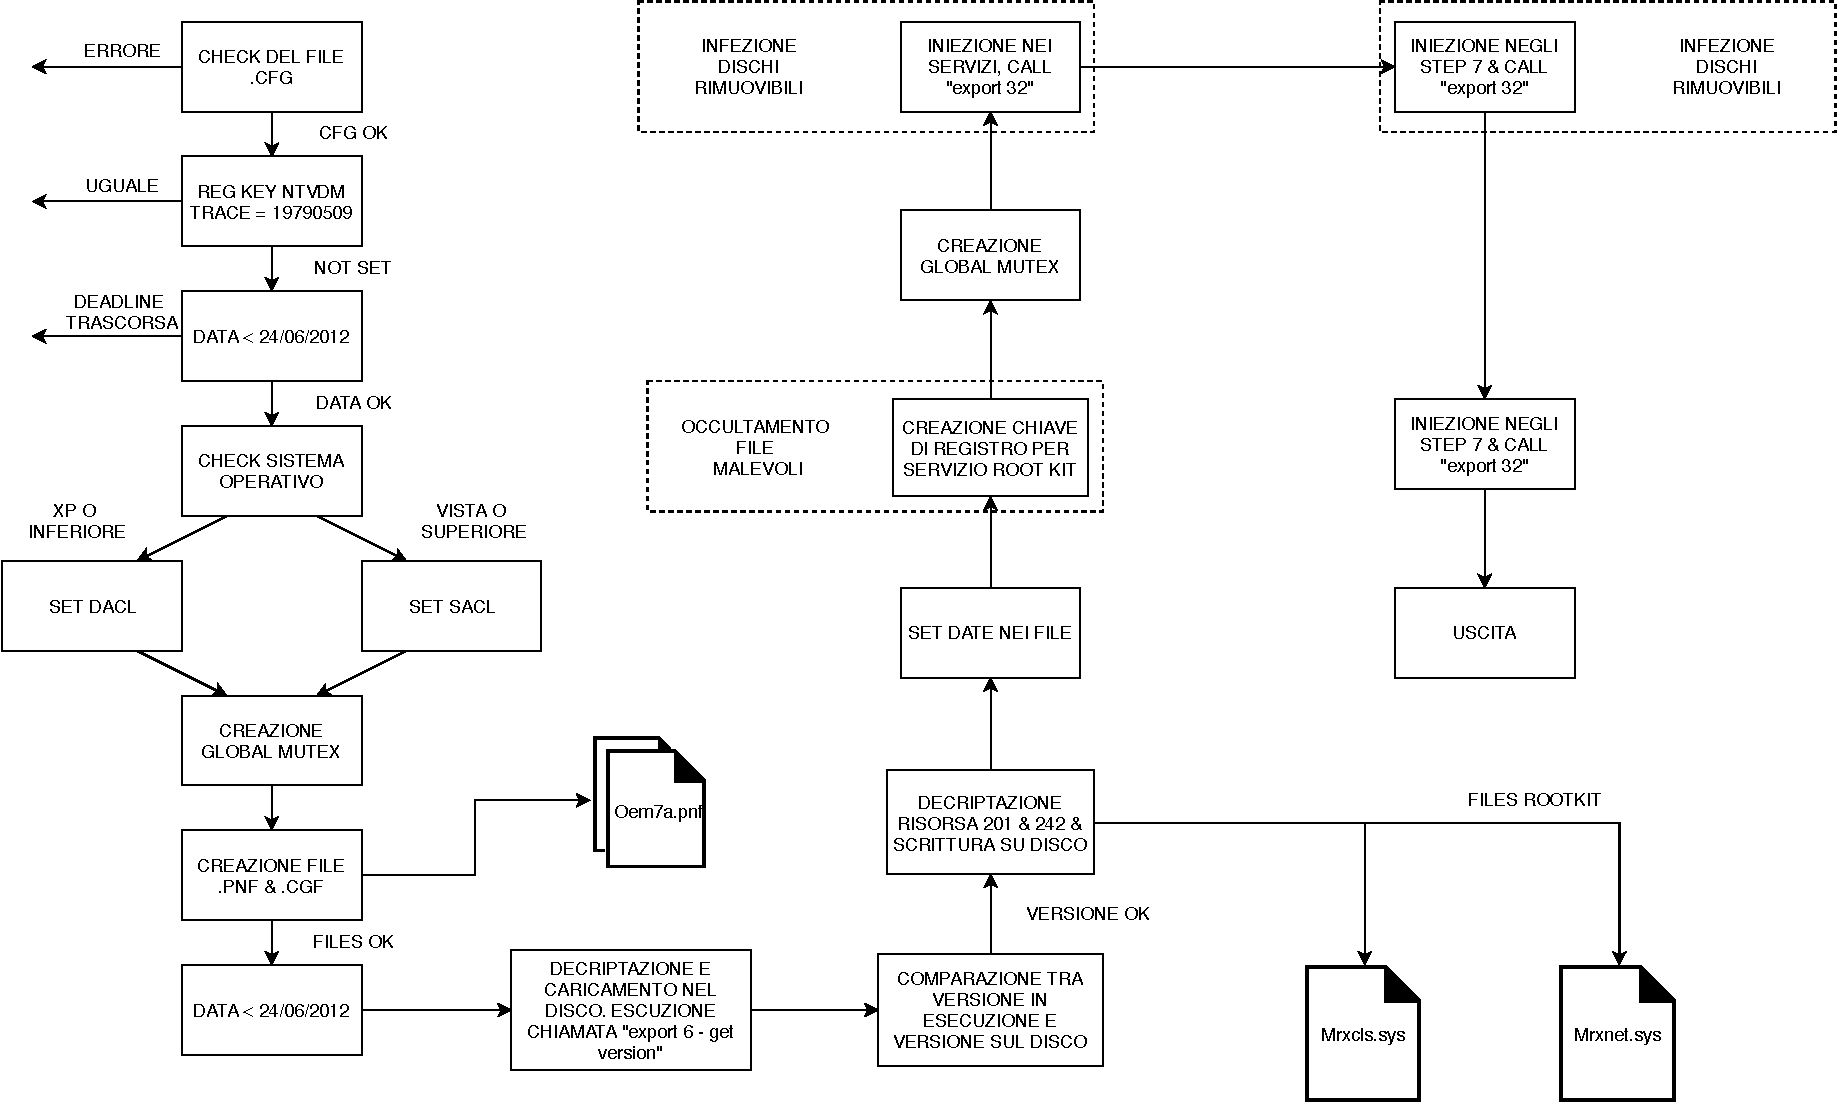
\includegraphics[scale=0.55]{Immagini/stuxnet_tree.pdf}}
\caption{Processo di infezione di Stuxnet (fonte \cite{Knapp_2015_7})}\label{fig:stuxnet_tree}

\end{figure}

Ma, nonostante i vari problemi che Stuxnet ha provocato nel periodo in cui � stato operativo, la sua comparsa ha permesso in realt� di comprendere molti limiti e difetti dei sistemi di sicurezza che fino al quel momento erano stati applicati per proteggere un sistema SCADA. Grazie agli studi condotti su Stuxnet, si � capito che molti dei paradigmi di sicurezza su cui venivano basate le architetture dei sistemi ICS erano errati e dovevano essere rivisti. Inoltre si � reso necessario concepire nuove misure di sicurezza per difendersi dalle nuove minacce basate sullo stesso paradigma operativo di Stuxnet. Nella tabella \ref{tab:stuxnet_differences} sono riportati nel dettaglio alcune delle differenze tra i paradigmi di sicurezza prima e dopo l'avvento di Stuxnet.

%tabella differenze
\begin{table}[tbh]
\begin{tabularx}{\textwidth}[c]{@{}XX@{}}
\toprule
\textbf{PARADIGMI PRE-STUXNET} & \textbf{PARADIGMI POST-STUXNET} \\ \midrule
I sistemi possono essere isolati efficacemente dalle reti esterne, eliminando il rischi di incidenti informatici & I sistemi di controllo sono ancora soggetti alla natura umana: un forte perimetro difensivo pu� sempre venire oltrepassato a causa della superficialit� nel trattare la sicurezza \\ \midrule
I PLC che non eseguono sistemi operativi moderni non sono vulnerabili agli attacchi informatici & I PLC possono essere degli obiettivi concreti per i malware \\ \midrule
I macchinari utilizzati per operazioni speciali beneficiano del paradigma "security through obscurity". Dato che la documentazione degli ICS non � disponibile, � impossibile creare un attacco contro di loro & Le risorse per creare un attacco di successo ed altamente specializzato contro un ICS sono tutte a disposizione degli hacker \\ \midrule
Per proteggere la rete di un ICS da un attacco � sufficiente l'utilizzo di firewall e IDS & L'utilizzo di molteplici vulnerabilit� allo zero-day per effettuare un attacco indicano che i metodi difensivi basati su blacklist non sono pi� sufficienti ed occorre considerare tecnologie basate su whitelist per difendersi contro delle vulnerabilit� ancora sconsociute \\ \bottomrule
\end{tabularx}
\caption{Differenze dei paradigmi difensivi SCADA prima e dopo l'avvento di Stuxnet (fonte: \cite{Knapp_2015_7})}
\label{tab:stuxnet_differences}
\end{table}

\subsection{Dragonfly}

Nel giugno del 2014, la compagnia finlandese di sicurezza informatica F-Secure post�, all'interno del proprio blog, la notizia della scoperta di un malware, descrivendo come lo stesso era stato utilizzato fino ad allora per scopi di sabotaggio ed acquisizione dati sensibili \cite{FSecure_2014}. Furono condotti subito un serie di studi da parte della Symantec, altra azienda dedita alla sicurezza informatica, culminati nella creazione di un report tecnico sulle modalit� operative del malware \cite{Symantec_2014}. La prima cosa scoperta fu che il malware era il frutto di una campagna di spionaggio iniziata nel 2010. Inizialmente gli obbiettivi erano industrie legate all'aviazione e alla difesa localizzate negli USA e in Canada, ma successivamente la campagna venne rivota contro compagnie del settore energetico, propagandosi anche al di fuori del continente americano \cite{Nelson_2016}. Ma la scoperta pi� significativa fu che, come nel caso di Stuxnet, Dragonfly era stato appositamente programmato per colpire dispositivi ICS, rappresentando il secondo caso di un malware creato esclusivamente per colpire i sistemi informatici degli impianti industriali.

La campagna di attacco ai danni delle industrie energetiche di Dargonfly si � sviluppata in tre fasi, sfruttando in ognuna di essa un vettore d'attacco differente:

\begin{enumerate}

\item nella prima fase, iniziata a febbraio 2013, fu impiegata la tecnica di spear phishing per infettare i computer delle vittime ed ottenere informazioni sensibili riguardanti la rete informatica dell'azienda da colpire. Tramite l'invio di file .PDF corrotti, veniva installato nelle macchine delle vittime un ``Remote Access Trojan Horse (RAT)'', ossia un malware con cui � possibile ottenere il controllo amministrativo da remoto del computer;

\item la seconda fase cominci� subito dopo la prima, nel maggio 2013, e si protrasse per circa 11 mesi, fino ad aprile 2014. Durante questo periodo furono utilizzati attacchi di watering hole. Questo attacco consiste nel dirottare la connessione di un utente verso un sito, portandolo a vistarne un altro, senza che la vittima se ne accorga. Il gruppo gestore di Dragonfly riusc� a dirottare il traffico internet delle aziende attaccate verso siti gestiti direttamente da loro. All'interno di questi siti veniva caricato il software malevolo che veniva installato sulla macchina di chiunque visitasse la pagina in questione;

\item per la terza ed ultima fase cominci� nel giugno 2013 e venne portata avanti in contemporanea con la seconda. In questa fase, gli hacker di Dragonfly riuscirono a attaccare i siti di supporto di alcune note aziende produttrici di componenti per ICS. In questa maniera riuscirono a sostituire i software legittimi delle compagnie con programmi creati da loro e contenenti sempre il codice malware che era stato diffuso con gli altri due metodi.

\end{enumerate}

La complessit� di questo attacco fa ben capire della profonda organizzazione che ci fu alle spalle.Il malware utilizzato serviva ad ottenere informazioni sui dispositivi ICS presenti nella rete, per oi inviarlo agli stessi creatori di Dragonfly. Anche in questo caso, come per Stuxnet, il sfotware malevolo era stato programmato per ricercare delle specifiche configurazioni hardware, di cui sfruttava alcune vulnerabilit� zero-day. Per farlo, utilizzava lo stesso protocollo industriale di comunicazione impiegato dai dispositivi ICS ricercati.

La scoperta di Dragonfly ha avuto un impatta nel mondo della sicurezza industriali paragonabile a quello che provoc� Stuxnet quattro anni prima. La campagna di attacco attuata dalla compagnia creatrice del malware ha sottolineato, di nuovo, alcuni limiti nell'organizzazione della difesa:

\begin{itemize}

\item la strategia ``Offense in Depth'' ha sicuramente giocato un ruolo importante nella diffusione del malware. Le organizzazioni vittime sono state attaccate su pi� livelli della loro infrastruttura;

\item le macchine colpite avevano installato tutte la stessa versione di Windows XP e sfruttava alcune vulnerabilit� del sistema operativo al zero-day;

\item Dragonfly fin� per essere installato sui dispositivi mobile del personale, che devono essere ormai considerati dei potenziali punti d'ingresso per le minacce;

\item nella campagna furono coinvolte anche le aziende produttrice, considerate fonte di software fidato. � necessario, quindi, controllare anche il traffico rivolto verso queste aziende, in quanto anche loro possono essere potenziali punti d'ingresso per delle minacce;

\item il malware ha operato indisturbatamente sulle macchine infettate per circa un anno senza mai venire scoperto dai software che monitoravano il traffico internet.

\end{itemize} 

Inoltre c'� da sottolineare come le aziende colpite, attualmente, rischino di subire degli ulteriori attacchi che sfruttano tutte le informazioni raccolte grazie a Dragonfly. A causa di tutto ci� si � reso necessario sviluppare un paradigma di sicurezza che tenesse conto dell'integrit� non solo dei dispositivi ICS ma anche della rete informatica tra gli stessi, sfruttando, ad esempio, schemi per la segmentazione di rete che permettono un controllo del traffico dati pi� accurato e completo.
\newpage

%tabella riassuntiva delle tipologie di attacchi
\scalebox{0.5}{}{\LTXtable{\textwidth}{Tabelle/threat_table}}

\chapter{SimSCADA: design e implementazione}

In questo capitolo verranno esposte le motivazioni che hanno portato allo sviluppo di SimSCADA. Inizialmente verranno illustrate le idee che si trovano alla base dello sviluppo del gioco. In seguito verranno mostrate le scelte di design e progettazione prese durante l'implementazione del progetto. Verranno descritte alcune delle dinamiche base presenti nel gioco e come sono state sviluppate. Verr� illustrato quali lezioni sono state inserite nel gioco e come possono essere apprese dal giocatore. Infine verr� mostrato come � stato realizzata la raccolta dati per monitorare e valutare le prestazioni del giocatore.

\section{Scelte di game design}

\subsection{Perch� i sistemi SCADA}

Il gioco � stato sviluppato come parte pratica di una tesi magistrale. Vista le difficolt� che possono nascere durante la creazione di un videogioco, si � cercato principalmente di creare un concept di ci� che potrebbe essere uno strumento di formazione in ambito di sicurezza informatica. Questa � una materia che pu� coinvolgerne molte altre. � stata necessaria, quindi, un'attenta analisi iniziale sia dei serious games a tema di sicurezza informatica gi� presenti nel mercato che di altri lavori precedentemente sviluppati (anche non commercializzati). Da questa analisi � scaturita l'assenza di uno strumento del genere applicabile in un contesto industriale e che andasse a coinvolgere i sistemi SCADA. Si � deciso quindi di rivolgere l'attenzione verso questo mondo che, a causa di una percezione influenzata ancora dalle idee del passato, viene ancora considerato come sicuro e privo di minacce, anche se gli episodi registrati negli ultimi anni descrivono un quadro ben diverso.

Il mondo dei sistemi SCADA � caratterizzato da una elevata variet� di fini applicativi: si va dal sistema di controllo per impianti industriali a quelli per il controllo dei trasporti automatizzati, passando per impianti di produzione energetica (centrali nucleari, gasdotti, ecc.). Piuttosto che focalizzarsi solo su una delle molte applicazioni per sistemi del genere, si � preferito mantenere un'ambientazione pi� generica. Questo � stato fatto principalmente per due motivi:

\begin{itemize}

\item innanzitutto riprodurre solo un determinato campo in maniera fedele avrebbe limitato in qualche modo il bacino d'utenza finale;

\item l'intento principale per cui � stato sviluppato il gioco � quello di cercare di educare il giocatore a prendere delle decisioni mirate ed oculate sia in maniera preventiva che al momento dell'emergenza, cercando di dare maggior importanza alle azioni che l'utente deve attuare rispetto agli effettivi strumenti utilizzati, in quanto differenti da situazione a situazione;

\item per aiutare a mantenere il tipo di ambientazione scelto, si � evitato di inserire rimandi a software e tecnologie specifici utilizzati in ambienti SCADA, in quanto questi si differenziano da situazione a situazione, a seconda del processo da controllare, l'impianto su cui si agisce e tutti gli altri elementi che sono stati elencati in \ref{sec:architecture}.

\end{itemize}

Ai fini di non ridurre in maniera eccessiva l'utenza finale, si sono inserite all'interno del gioco delle nozioni su cosa sia un sistema SCADA ed altre informazioni relativi ad essi, oltre a tutte le lezioni riguardanti i pericoli e gli attacchi informatici a cui un sistema di questi tipo pu� essere sottoposto. Sono poi presenti le lezioni sugli attacchi informatici che sistemi di questo tipo possono subire e quali azioni si possono effettuare per mitigare delle situazioni potenzialmente pericolose.

\subsection{La tipologia di gioco: tycoon}

Per ottemperare all'intento prefissato di dar risalto alle azioni che l'utente deve intraprendere durante la propria partita, si � scelto di sviluppare un gioco di genere gestionale o tycoon, ispirandosi in particolar modo alla serie di titoli di questo genere sviluppati nel corso degli anni, quali ``Roller Coaster Tycoon'' e ``SimCity''. Lo scenario tipico di questi giochi prevede che l'utente si trovi a capo di una determinata realt� economica (un parco di divertimento, una citt� e cos� via, a seconda dell'ambientazione) e deve cercare di gestirla nel migliore dei modi (portandola ad esempio ad aumentare gli incassi o completando altri obiettivi imposti dal sistema), cercando di far fronte con le proprie azioni ai vari problemi che si presentano nel corso della partita.

Da questo punto di vista, si � cercato di riprenderne anche l'impostazione grafico, adottando uno stile retro, di rimando alle versioni dei suddetti titoli sviluppati a cavallo degli anni `80 e `90 (periodo caratterizzato da un massiccio sviluppo di questa tipologia di giochi). Inoltre questo stile permette di mantenere il gioco leggero, graficamente parlando, rendendolo utilizzabile anche su macchine con basse performance. 

\subsection{La piattaforma di destinazione: WebGL}

La piattaforma su cui far eseguire il gioco una volta completato � stata oggetto di diverse analisi. Nella fase iniziale di sviluppo, si era deciso di implementare il gioco per piattaforma Windows, essendo questo il sistema operativo pi� diffuso, soprattutto in ambito di videogames. Durante lo sviluppo del gioco, per�, � stato considerato che, sebbene diffusa, sviluppare il gioco solo per piattaforma Windows sarebbe stato comunque limitante per lo scopo finale del progetto. � stato deciso, quindi, di cambiare la piattaforma di destinazione, affidandosi all'utilizzo delle API WebGL.

Queste interfacce di programmazione, scritte in linguaggio JavaScript, permettono l'esecuzione di applicazioni 2D e 3D tramite web browser, senza richiedere l'utilizzo di alcun tipo di plug-in da parte dell'utente, facendo eseguire il codice relativo alla componente grafica direttamente alla GPU del sistema utente. Sono state rilasciate inizialmente nel 2011 e da allora si sono diffuse largamente, venendo integrate da altri standard web. Recentemente diversi motori grafici hanno iniziato a supportarne lo sviluppo (Unity e Unreal Engine tra i pi� famosi) permettendo ulteriormente il diffondersi di questa tecnologia.

Le ragioni per cui � stato effettuato il cambio della piattaforma sono diverse, quelle che hanno avuto un peso maggiore nella decisione sono state:

\begin{itemize}

\item la tecnologia WebGL pu� essere eseguita su qualsiasi sistema, a prescindere dal sistema operativo installato su di esso. Basta, infatti, l'utilizzo di un web browser che ne supporti l'utilizzo (ovviamente il sistema deve essere sufficientemente potente per garantire il corretto funzionamento del gioco, ma nel caso in questione non ci si � soffermati pi� di tanto su questo aspetto, in quanto il gioco presenta una grafica molto minimale che non richiede un utilizzo eccessivo di risorse da parte del sistema);

\item dovendo effettuare una raccolta dati sulle performance del giocatore, in modo da poter estrapolare successivamente i dati che permettano di capire se l'apprendimento del giocatore sta avvenendo in maniera corretta, utilizzare una tecnologia web, come appunto WebGL, permette una gestione pi� semplice di questo aspetto. Infatti, mentre il codice grafico � eseguito in locale, il codice di controllo del gioco viene eseguito dal server su cui � stato caricato. Per la raccolta dati, quindi, � stato sufficiente creare i file necessari all'interno del server e collezionarli, senza richiedere alcun tipo di azione da parte del giocatore.

\end{itemize}

\subsection{Il motore di gioco: Unity}

La scelta della piattaforma di sviluppo � stata presa senza troppi dubbi, contrariamente agli altri aspetti fin'ora esposti. Subito, infatti, � stato deciso di sviluppare il gioco grazie all'ausilio del software Unity, un motore grafico multipiattaforma, che permette la creazione di applicazioni grafiche sia 2D che 3D. Inizialmente si � tentato di approcciare lo sviluppo del gioco tramite l'utilizzo del framework Phaser.io, ma questa idea � stata rapidamente scartata per diversi motivi tra cui:

\begin{itemize}

\item Phaser.io � un framework di gioco nato di recente e creato unicamente per applicazioni 2D. Unity, d'altro canto, � un motore grafico in circolazione da molto pi� tempo e che permette di sviluppare applicazioni sia in 2D che in 3D. Dato che lo stile grafico del gioco � stato deciso solamente in un secondo momento, avere una piattaforma di sviluppo che non ponesse dei limiti da questo punto di vista � stato decisivo;

\item il fatto che Unity abbia un tempo di vita maggiore, fa si che esistano molti pi� asset grafici, sviluppati da terze parti, liberamente utilizzabili e che hanno permesso di velocizzare lo sviluppo in alcuni momenti;

\item Unity permette di cambiare la piattaforma di destinazione, a prescindere dal codice che si � prodotto fino a quel momento. Questa funzionalit� � stata presa in considerazione nella scelta ed � stata, come si � visto, sfruttata durante lo svolgimento del lavoro;

\item Unity permette di sviluppare codice in diversi linguaggi di programmazione (C, C++, C\#) mentre Phaser.io � scritto solamente per linguaggio JavaScript. Data la maggior familiarit� dello sviluppatore con il linguaggio C\# (utilizzato poi nello sviluppo del codice), Unity � sembrata la scelta pi� adatta per iniziare in maniera pi� veloce lo sviluppo del gioco.

\end{itemize}

\subsection{L'IDE: Visual Studio}

Per quanto riguarda l'IDE di sviluppo, la scelta di Unity come motre grafico ha condizionato in maniera decisiva la scelta di quest'ultimo. Sebbene, infatti, sia possibile utilizzare qualsiasi IDE che permette lo sviluppo di codice C\#, Visual Studio, a differenza degli altri software, possiede diverse integrazioni con il motore in questione che sono di supporto nello sviluppo, rendendo di fatto questa scelta quasi obbligata. 

\section{La raccolta dati}

Prima di iniziare lo sviluppo del gioco, � stata affrontata una fase di raccolta dati. Lo scopo era quello di individuare quale fosse il modo migliore per rappresentare l'ambiente SCADA all'interno di un videogioco. In particolare si voleva evitare di rendere il gioco troppo tecnico e complesso da punto di vista operativo, in quanto avrebbe limitato, come detto, il bacino di utenza finale e sarebbe stato eventualmente di difficile comprensione per il giocatore.

L'idea di gioco iniziale era quella di creare un simulatore di un sistema SCADA. Il giocatore avrebbe interagito con esso tramite l'interfaccia HMI e avrebbe dovuto fronteggiare diversi tipi di attacchi informatici. Per questo motivo sono stati presi in esame una serie di software per interfacce HMI, tra cui WinLog CC e STEP7. Quest'ultimo, in particolare � sviluppato dalla Siemens e fa parte della famiglia di prodotti Simatic, comprendente sia software che hardware per il controllo di sistemi di automazione. Analizzati i software, per� si � capito che emulare un sistema SCADA sarebbe stato complesso, in quanto era necessario dover programmare i diversi PLC che avrebbero controllato il processo (emulato anch'esso tramite computer). 

Scartata quindi l'ipotesi dell'emulatore, si � deciso di porre il focus del gioco sulle diverse minacce che possono coinvolgere un sistema SCADA. Dalle ricerche svolte, infatti, sugli attacchi informatici effettuati ai danni di un sistema di controllo, � emerso che esiste ancora l'errata convinzione di ritenere l'ambiente SCADA sicuro dagli attacchi esterni in quanto tecnologicamente diverso, senza rendersi conto che, in realt�, con il passare degli anni le tecnologie del mondo domestico sono entrate a far parte di quello industriale, rendendoli molto pi� simili di quanto si pensi.

Partendo da ci�, � stata formulata l'idea di un gioco gestionale in cui l'utente si trova a gestire la sicurezza di un ambiente SCADA, fronteggiando diversi tipi di attacchi e cercando di prevenire il fallimento economico per colpa di essi.

\section{La storia nel gioco}

Il gioco si sviluppa all'interno di una societ� fornitrice di servizi SCADA. Il giocatore � stato appena messo a capo del reparto di sicurezza e dovr� gestire i vari aspetti legati ad essa. Quindi non dovr� solo evitare di subire attacchi informatici, ma avr� il compito anche di scovare eventuali infiltrati tra i dipendenti che si troveranno a lavorare all'interno dei locali da proteggere.

Ma mano che riuscir� a difendere i sistemi aziendali, il giocatore guadagner� soldi e aumenter� la propria reputazione. Questo gli permetter� di acquistare migliorie difensive per aiutarlo nel proprio compito. Una volta raggiunto un livello di reputazione e soldi sufficientemente alto, lo scenario si concluder� con la vittoria e si potr� accedere la secondo livello, in cui dovr� fronteggiare minacce pi� pericolose. Se, invece, non dovesse riuscire a proteggere l'azienda dagli attacchi e subisse troppi attacchi, con relative perdite economiche, il gioco terminer� con una sconfitta e il giocatore dovr� ricominciare lo scenario dall'inizio.

La storia � stata mantenuta molto basilare in quanto, tipicamente, nei giochi gestionali non ha una particolare rilevanza. In questo tipo di giochi vi sono, usualmente, degli obiettivi che il giocatore pu� completare nel corso del gioco (raggiungere un determinato livello di introiti economici, effettuare un determinato numero di azioni positive, ecc.), ma in questo caso sono stati estromessi nella programmazione per questioni legate al tempo necessario per idearle ed implementarle.

\section{Contenuto del gioco}

\subsection{Game tutorial}

\subsection{Le lezioni}

\section{Gestione degli asset di gioco}

\section{Implementazione delle routine per le AI}

\chapter{Manuale dello sviluppatore}

In questo capitolo sono inserite tutte le informazioni necessarie per chiunque voglia modificare la struttura del gioco, aggiungendo livelli, minacce, messaggi e quant'altro. Nella prima parte � esposta la modalit� di installazione del gioco, in modo da riuscire ad eseguirlo in locale con fini di sviluppo \ref{sec:howto}. Successivamente, nei paragrafi \ref{sec:noncodecontents}, \ref{sec:classes} e \ref{sec:prefabs} sono fornite informazioni riguardo sia i file di codice che non, utilizzati all'interno del gioco e su cui eventualmente agire per apportare modifiche riguardo la logica del gameplay. In \ref{sec:folderstructure} � mostrata la struttura delle cartelle di gioco, esposta cos� come appare all'interno dell'editor di Unity. Infine, nell'ultima sezione (\ref{sec:addlevel}) � esposto come � possibile aggiungere dei livelli al gioco.

\section{Guida d'installazione}\label{sec:howto}

Il gioco, al momento della stesura di questo report, � disponibile all'indirizzo \url{http://simscada.sfcoding.com/SIMSCADA/}. Se non dovesse essere pi� disponibile, � possibile eseguirne una versione in un server locale. Questo pu� essere utile anche per effettuare test in caso di modifiche del codice di controllo, aggiunte di livelli e cos� via. Per far s� che il gioco funzioni in locale, per�, sono necessari alcuni passaggi.

\begin{description}

\item[Installazione di un server di gioco] Per eseguire il gioco, � sufficiente avere un web server Apache installato sulla propria macchina e copiare i file prodotti da Unity al momento della build, ossia il contenuto delle cartelle \cmd{Build} e \cmd{TemplateData}, pi� il file \cmd{index.html}, all'interno della cartella \cmd{htdocs} del server. Esistono diversi metodi per installare un server Apache, a seconda anche del sistema operativo su cui si sta lavorando, ma una soluzione veloce, semplice e soprattutto valida per tutti i casi � quella fornita dal software \cmd{XAMPP}. 

Questo software, disponibile al link \url{https://www.apachefriends.org/it/download.html}, � disponibile per Windows, MacOS e Linux e permette di installare velocemente tutte le componenti necessarie per eseguire un web server sulla propria macchina in locale. 

Una volta terminata la procedura d'installazione di \cmd{XAMPP}, sar� necessario individuare la cartella dove sono stati salvati i file. Normalmente, quelle predefinite sono:

\begin{description}

\item[Windows:] C:/xampp

\item[Linux:]  /opt/xampp

\item[MacOS:]  /Applications/XAMPP/xamppfiles

\end{description}

\item[Creazione della cartella di gioco] Trovata la cartella di installazione di \cmd{XAMPP}, sar� necessario individuare la cartella\cmd{htdocs}. Al suo interno � consigliato creare un'ulteriore cartella, denominata ad esempio \cmd{SIMSCADA}. Qui dovranno essere copiati tutti i file prodotti da Unity al momento della build.

\item[Download del progetto] � possibile ottenere

\item[Installazione di Unity]

\item[Creazione della build]

\item[Copia della build nel server]

\end{description}

\section{Contenuti del gioco senza codice}\label{sec:noncodecontents}

\section{Classi}\label{sec:classes}

\section{Prefab}\label{sec:prefabs}

\section{Struttura delle cartelle}\label{sec:folderstructure}

\section{Come aggiungere un livello}\label{sec:addlevel}

\chapter{Risultati}

\chapter{Conclusioni}

% bibliografia scritta "a mano"
%\input{biblio.tex}

% se la bibliografia � stata scritta (usando Bibtex) nel file biblio.bib allora commentare la riga precedente e scommentare le due righe seguenti
%\bibliographystyle{torsec}
%\bibliography{biblio}

\printbibliography

\end{document}
